%%%%%%%%%%%%%%%%%%%%%%%%%%%%%%%%%%%%%%%%%%%%%%%%%%%%%%%%%%%%%%%%%%%%
%%%%%%%%%%%%%%%%%%%%%%%%%%%%%%%%%%%%%%%%%%%%%%%%%%%%%%%%%%%%%%%%%%%%
%%                                                                %%
%% Esimerkki opinn�ytteen tekemisest� LaTeX:lla 20130926          %%
%% Alkuper�inen versio Luis Costa,  muutokset Perttu Puska        %%
%%                                                                %%
%% T�h�n esimerkkiin kuuluu tiedostot                             %%
%%               opinnaytepohja.tex (versio 1.7)                  %%
%%               aaltothesis.sty (versio 1.7)                     %%
%%               kuva1.eps                                        %%
%%               kuva2.eps                                        %%
%%                                                                %%
%%                                                                %%
%% K��nt�minen                                                    %%
%% latex:                                                         %%
%%             $ latex opinnaytepohja                             %%
%%             $ latex opinnaytepohja                             %%
%%                                                                %%
%%   Tuloksena on tiedosto opinnayte.dvi, joka                    %%
%%   muutetaan ps-muotoon seuraavasti                             %%
%%                                                                %%
%%             $ dvips opinnaytepohja -o                          %%
%%                                                                %%
%% Selitt�v�t kommentit on t�ss� esimerkiss� varustettu           %%
%% %%-merkeill� ja muutokset, joita k�ytt�j� voi tehd�,           %%
%% on varustettu %-merkeill�                                      %%
%%                                                                %%
%%%%%%%%%%%%%%%%%%%%%%%%%%%%%%%%%%%%%%%%%%%%%%%%%%%%%%%%%%%%%%%%%%%%
%%%%%%%%%%%%%%%%%%%%%%%%%%%%%%%%%%%%%%%%%%%%%%%%%%%%%%%%%%%%%%%%%%%%

%% modified Aalto Master Degree Thesis tamplate
%% author Liu Peng


%% Use one of these you write in Finnish:
%% the 1st when using pdflatex (use pdf figures) or
%% the 2nd when producing a ps file (use eps figures).
%\documentclass[finnish,12pt,a4paper,pdftex]{article}
%\documentclass[finnish,12pt,a4paper,dvips]{article}


%% Uncomment one of these if you write in English
\documentclass[english,12pt,a4paper,pdftex]{article}
%\documentclass[english,12pt,a4paper,dvips]{article}

%% This package is required
%% Choose your school from arts, biz, chem, elec, eng, sci.
%% Choose the character encoding scheme used by your editor: utf8, latin1
%\usepackage[elec,utf8]{aaltothesis} % this is the default in aaltothesis.sty
\usepackage[elec,latin1]{aaltothesis}


%%
%% Use this if you run pdflatex and use jpg/pdf-format pictures.
%%
\usepackage{graphicx}
\usepackage{subfigure}
\usepackage{titlesec} 

%% Use the macros in this package to change how the hyperref package below 
%% typesets its hypertext -- hyperlink colour, font, etc. See the package
%% documentation. It also defines the \url macro, so use the package when 
%% not using the hyperref package.
%\usepackage{url}


%% Use this if you want to get links and nice output with pdflatex
\usepackage[pdfpagemode=None,colorlinks=true,urlcolor=red,%
linkcolor=blue,citecolor=black,pdfstartview=FitH]{hyperref}


%% Use this if you write hard core mathematics, these are usually needed
\usepackage{amsfonts,amssymb,amsbsy}  

%% Vaakasuunnan mitat, �L� KOSKE!
\setlength{\hoffset}{-1in}
\setlength{\oddsidemargin}{35mm}
\setlength{\evensidemargin}{25mm}
\setlength{\textwidth}{15cm}
%% Pystysuunnan mitat, �L� KOSKE!
\setlength{\voffset}{-1in}
\setlength{\headsep}{7mm}
\setlength{\headheight}{1em}
\setlength{\topmargin}{25mm-\headheight-\headsep}
\setlength{\textheight}{23cm}


%% add chapter title depth to 4, use paragraph to represent subsubsubsection
\setcounter{secnumdepth}{4}
\titleformat{\paragraph}
{\normalfont\normalsize\bfseries}{\theparagraph}{1em}{}
\titlespacing*{\paragraph}
{0pt}{3.25ex plus 1ex minus .2ex}{1.5ex plus .2ex}

%% set up chapter title
\usepackage{parskip}
\titlespacing*{\section}
{0pt}{5.5ex plus 1ex minus .2ex}{4.3ex plus .2ex}

%% Output starts heref
\begin{document}


%% Change the school field to describe your school if the autimatically 
%% set name is wrong
% \university{aalto University}{aalto-Yliopisto}
% \school{School of Electrical Engineering}{S�hk�Tekniikan korkeakoulu}


%% Only for B.Sc. thesis: Choose your degree programme. 
%\degreeprogram{Electronics and electrical engineering}%
%{Elektroniikka ja s�hk�tekniikka}
%%


%% Only for M.Sc. and Licentiate thesis: Choose your department,
%% professorship and professorship code. 
\department{Department of Communications and Networking}%
{Radiotieteen ja -tekniikan laitos}
\professorship{Networking Technology}{Piiriteoria}
\code{S-38}
%%


%% Choose one of these:
%\univdegree{BSc}
\univdegree{MSc}
%\univdegree{Lic}


%% Should be self explanatory...
\author{Peng Liu}

%% Your thesis title. If the title is very long and the latex 
%% does unsatisfactory job of breaking the lines, you will have to
%% break the lines yourself with \\ control character. 
%% Do not hyphenate titles.
\thesistitle{Developing a Solution for Multimedia Home Networking}{ }

\place{Espoo}

%% For B.Sc. thesis use the date when you present your thesis. 
\date{20.5.2015}


%% B.Sc. or M.Sc. thesis supervisor 
%% Note the "\" after the comma. This forces the following space to be 
%% a normal interword space, not the space that starts a new sentence. 
\supervisor{Prof.\ Raimo A. Kantola}{Prof.\ Raimo A. Kantola}


%% B.Sc. or M.Sc. thesis advisors(s). 
%%
%% Note that there has been a change in the official EN translation
%% of the Finnish title ``ohjaaja'' which in the previous version (1.5) 
%% of this document was called ``instructor''. The recommended
%% translation is now ``advisor''.  
%% However, the LaTeX internal variable remains \instructor
%% as there is little point to change the variable name. 
%%
%\instructor{Prof. Pirjo Professori}{Prof. Pirjo Professori}
\instructor{D.Sc.\ (Tech.) Mikko Valimaki}{TkT Olli Ohjaaja}
%\instructor{M.Sc.\ (Tech.) Polli Pohjaaja}{DI Polli Pohjaaja}


%% Aalto logo: syntax:
% \uselogo{aaltoRed|aaltoBlue|aaltoYellow|aaltoGray|aaltoGrayScale}{?|!|''}
%% Logo language is set to be the same as the document language.
\uselogo{aaltoRed}{''}


%% Create the coverpage
\makecoverpage


%% Force new page so that English abstract starts from a new page
\newpage
%
%% English abstract, uncomment if you need one. 
%% 
%% Abstract keywords
\keywords{Home network, Multimedia, HTTP Streaming,\\ UPnP, DLNA, Miracast, AirPlay}
%% Abstract text
\begin{abstractpage}[english]

%% Abstract chapter
%% author Liu Peng
In recent years, the rapid development of electronics and computer science has
enabled home networking devices to become more affordable and more powerful.
Several widely used multimedia-streaming solutions have become available in the
market. However, these standards are not compatible with each other. Moreover,
even devices using the same standard are not always compatible with each other,
since the implementation approaches may vary from device to device.

This thesis compares the modern solutions for multimedia home networking (MHN),
including AirPlay, Digital Living Network Alliance (DLNA), Miracast, and
Chromecast standards. By analyzing the features and capabilities of these
streaming technologies, this thesis proposes a universal solution for MHN to
support multiple protocols and bridge different platforms.

Based on this thesis, different multimedia solutions were tested and a mobile
application for home networking was implemented on the Android operating system.
Over 16 months after the launch of this application on the Google Play Store,
the application received over one million downloads from 225 countries.
Over 10000 users rated the application, and near half of the users gave it 5
stars. This solution has proved to be competitive and successful.

The thesis also proposes a plan for future development of this solution,
including the support for more platforms, independent streaming SDK, and
performance optimization. In addition, this thesis discusses the future trends
of home networking, which is more connected and cloud based.


\end{abstractpage}
%% Note that 
%% if you are writting your master's thesis in English place the English
%% abstract first followed by the possible Finnish abstract

%% Preface
%\mysection{Esipuhe}
\mysection{Preface}

%% Preface chapter
%% author Liu Peng

This document is my Master's thesis for \textit{Communications Engineering, majoring in
Networking} at Aalto University. All research and development of this thesis was
conducted at Tuxera Inc. in Helsinki from January 2013 to June 2014. Tuxera is a
high-tech startup that develops kernel-level file systems and multimedia solutions
for leading software, hardware and electronics companies.

During this project, I worked together with my colleagues at Tuxera, starting
to work on the DLNA project in the first few months during which time I learned
the DLNA architecture and conducted the research about Digital Media Server
solutions. After that, I worked on an Android project to develop a universal
solution for multimedia home networking.


\mysection{Acknowledgements}

%% Acknowledgements chapter
%% author Liu Peng

First of all, I would like to thank the Streambels team at Tuxera, with whom I worked
together throughout the project. I would like to thank Karthik Ramakrishna, our
lead developer. Every week, he helped solve problems in the project.
No matter whether the question was theoretical or technical, he always answered my
questions. As our project manager, Oscar Santolalla helped us with
the organizational problems that we encountered and taught us to look from the
end-user perspective as well. Sakari Tanskanen, our mobile developer helped us
by integrating Chromecast and FireTV support for Streambels. Nadir Javed, our
quality assurance engineer helped us with the quality management and testing of
potential bugs before releasing the product to end users. Karolina Mosiadz, our
Public Relations Manager listened to user feedback every day and provided the unique
insights to improve Streambels. Hien Le, our UX designer helped us to develop
a quite intuitive user interface. And special thanks to Mikko V{\"a}lim{\"a}ki
and Szabolcs Szakacsits who led the company and gave me the opportunity to participate in
this great project. Without them, I would not have been able to finish this
report.

I thank my university supervisor Raimo Kantola, who helped me to develop a good
thesis topic based on my project and helped me with initial problem description.
I received great support from him with his constructive criticism and useful
advice, especially during the middle and final phase, when I wrote the report.

Finally, I thank everybody who supported me during my graduate work,
especially my family, friends, and housemates.

\vspace{4cm}
%\vspace{5cm}
Otaniemi, 20.5.2015

\vspace{5mm}
{\hfill Peng\ Liu \hspace{1cm}}


%% Force new page after preface
\newpage


%% Table of contents. 
\thesistableofcontents

\newpage
\listoffigures
 
\newpage
\listoftables
%% Symbolit ja lyhenteet
%%
%% Symbols and abbreviations
%\mysection{Symbolit ja lyhenteet}
\mysection{Abbreviations}

%% Abbreviations chapter
%% author Liu Peng

%\subsection*{Symbolit}

%\subsection*{Operaattorit}

%\subsection*{Lyhenteet}
%\subsection*{Abbreviations}

\begin{tabular}{ll}
MHN	   & multimedia home networking \\
DLNA       & Digital Living Network Alliance\label{dlna_shortfor} \\ 
DMC        & Digital Media Controller \\
DRM        & Digital Rights Management \\ 
DMS        & Digital Media Server \\
DMR        & Digital Media Renderer \\
HTTP       & Hyper Text Transfer Protocol \\
RTSP       & Real Time Streaming Protocol \\
SDP    	& Session Description Protocol\\ 
UPnP	   & Universal Plug and Play \label{upnp_shortfor} \\
DIAL	   & DIscovery And Launch \label{dial_shortfor} \\
AP	   & Access Point \\
RAOP	   & Remote Audio Output Protocol\\
GENA		& General Event Notification Architecture\\
SOAP		& Simple Object Access protocol\\
DRM		& Digital Rights Management\\
DIS		& DRM Interoperability Solutions\\
REST		& Representational State Transfer\\
URL		& Uniform resource Locater \\
XML		& Extensible Markup Language \\
\end{tabular}



%% Corrects the page numbering, there is no need to change these
\cleardoublepage
\storeinipagenumber
\pagenumbering{arabic}
\setcounter{page}{1}


%% Leip�teksti alkaa
%%
%% Text body begins. Note that since the text body
%% is mostly in Finnish the majority of comments are
%% also in Finnish after this point. There is no point in explaining
%% Finnish-language specific thesis conventions in English.
%\section{Johdanto}
\vspace*{100px}
\section{Introduction}

%% Ensimm�inen sivu tyhj�ksi
%% 
%% Leave first page empty
\thispagestyle{empty}

%% Introduction chapter
%% autor Liu Peng

\subsection{Home networking}
People's lives are being digitalized. This digitalization can be seen in the
increasing number of home multimedia devices, such as digital TVs, smart
phones, digital cameras, tablets, PCs, laptops and NAS (Network Attached
Storage), which are all equipped with ever greater processing power and mass
storage, wielding the power to record our daily lives and handle multimedia
information. The digitalized world has also seen rapid growth in network
deployment.  In this digitalized world, networking is being rapidly adopted at
homes. For example, in the U.S. in 2009, approximately 63\% of the homes had
already gained access to a broadband connection \cite{stateofHN}. Over 50\% of
these households had even installed their own "home network", which is defined as
multiple computers or devices sharing a broadband connection via either a wired
or wireless connection within the home \cite{standards-perspective}. In a typical home
scenario, most of these devices are connected to a local network, such as a
Wi-Fi hot spot, in order to allow music, pictures, videos and other content to
be ported across different devices.

\subsection{Motivation and Aims}
While the adoption of home networks has steadily increased since the late 1990s
and early 2000s, home networks have indeed encountered problems and limitations
\cite{stateofHN}. For example, the usability of home-networking technologies has
become a key impediment to the adoption of new applications in the home, since the
home-networking technology was originally developed for research labs and
enterprise networks and does not account for the unique characteristics of home
usage, such as the lack of professional administrators, deep heterogeneity, and
expectations of privacy. Among all the challenges of home-networking,
connecting all media devices and making them work together is becoming
increasingly interesting because of the rapid growth of consumer electronics
markets. Although several widely used multimedia-streaming solutions have
become available in the market, the standards employed are not compatible with
each other. Moreover, even devices using the same standard are not always
compatible with each other, since the implementation approaches may vary from
device to device. These incompatibilities are causing great inconvenience to
the end users.\\
\\
Currently, four major multimedia home network digital living solutions  are
deployed: AirPlay, Miracast, DLNA, and Chromecast. AirPlay is only used
between Apple products; it provides various features, including iTunes for
playing music as well as AirPlay for video, photos and screen mirroring.
Miracast (previously called Wi-Fi Display) was proposed by the Wi-Fi Alliance
and has received great popularity over recent years. Since its release version
4.2.2, Miracast has officially supported the Android operating system. Of the
four standards, DLNA has become the most widely deployed solution, with 2.2
billion installations worldwide. DLNA was proposed by several industrial
leading electronic manufacturers and network operators, including AT$\&$T,
Broadcom, Cisco, Google, Huawei, Intel, LG Electronics, Microsoft, Nokia,
Panasonic, Samsung, Sony and Verizon.\\
\\
As a result of their different technical designs, these standards proposed by
individual device manufacturers naturally experience serious compatibility
issues. Thus, end users can have several multimedia devices, with each one
using a distinctive, unique protocol, making it challenging or even impossible
sometimes to share media between those devices. These compatibility issues have
motivated the need to determine the technological features common to the four
multimedia-streaming standards and to develop a more easy-to-use multimedia
home networking solution based on more advanced technologies.

\subsection{Structure of the thesis}
The remainder of this thesis is divided into four chapters. Chapter
\ref{chapter2} provides an overview of popular home networking standards
currently in use. After a short comparison of these solutions, Chapter
\ref{chapter3} develops and proposes a more universal solution for multimedia
home networking and its implementation.
Chapter \ref{chapter4} evaluates the streaming performance of our solution and
presents some recent statistics from the Google Store to demonstrate the
compatibility of the proposed solution. This chapter also presents a study
based on the user feedback in order to further improve this solution. In
Chapter \ref{chapter5}, the thesis is concluded by  discussing potential 
further developments and prospect of home networking. 

%% In a thesis, every section starts a new page, hence \clearpage
\clearpage

%\section{Aikaisempi tutkimus}
\vspace*{100px}
 \section{Background\label{chapter2}}
 
%% Background chapter 
%% author Liu Peng 

Home networking has been a hot topic for quite a few years. Thanks to the rapid development 
of electronics and computer science, home networking devices are becoming more affordable 
and more powerful than they ever were. It is now so common that a person would
have several multimedia devices that can be connected to the network. In this
chapter, we give an overview of current solutions of home networking that
bridges these multimedia devices. By making comparison among these solutions we
try to identify the challenges that face home networking.
\subsection{Overview} 
Early researches \cite{link_layer_old} \cite{end_user} \cite{link_layer}
conducted on home networking mainly aims to find out how home networking
infrastructures can be built. The subjects of these researches, including cable
connection, wireless connection, optical connection etc, concerns more about
the physical layer of the home network.  So far, it has turned out that the
IEEE 802.11 protocol stack, among all others, is the most successful and 
widely deployed home networking infrastructure.\\
\\
Nowadays, a typical scenario of home networking is that an IEEE 802.11
supportive wireless router connecting to a Ethernet cable or optical cable from
the network operator creates a local network and other user devices simply join
this network. The wireless Access Point(AP) employs the 802.11 b/g/n/ac
protocol, utilizing the 2.4 GHz or 5 GHz frequency channels and providing a
100+ Mbps  network connection, whose bandwidth is sufficient for transmitting
the popular High Definition (1080p) videos.\\
\\
In terms of network and application layer technologies, different device 
manufactures tend to choose their preferred multimedia-sharing protocols from
the pool of protocols that have been evolving and developing for a long time.\\
\\
Since late 1990s, UPnP protocol had been developed for home networking usage. 
At that time, XML was popular and widely used by different network applications.
Under such background, UPnP was designed to fully make use of XML. UPnP is 
independent of media types and devices and it runs on the TCP/IP stack, thus it can 
be easily applied to modern network infrastructures.\\
\\ 
In June 2003, Sony and several leading consumer electronic manufacturer s
established the Digital Living Network Alliance (DLNA), a nonprofit 
collaborative trade association. The DLNA standard is based on the widely used UPnP 
protocol but it added some restrictions on media formats and some compatibility 
requirements. A device hardware and software can be certified by DLNA 
organizations to prove that it can work with other devices that also passed 
this certification. \\
\\
In 2010, Apple quit DLNA and developed its own multimedia home networking 
solution, known as AirPlay. By adding screen mirroring, authentication and Remote 
Audio Output Protocol(RAOP) music streaming, Apple tried to forge a more advanced 
home network sharing system, aiming to provide a unique user experience among Apple 
products. Apple's solution had indeed attracted people's interest, and the user experience 
had proved much better than that of other similar products in the market. With its improvement
 over the years,  Apple's solution has now been acknowledged as one of the most popular streaming 
solutions.\\
\\
Two years later, Wi-Fi alliance released its Miracast technology, and 
participated in pushing new standard in wireless home networking. The Miracast 
uses the Wi-Fi direct technology and it does not require a wireless local 
network. Instead, a peer-to-peer connection is created between the sharing and 
receiving devices. After its release, some major software and hardware 
companies soon accepted this new standard. Google, for example integrated Miracast 
support into its Android operating system, and provided screen-mirroring feature 
to other Miracast receivers. \\
\\
The competition in home networking rages on over the years. In 2013, Google released a 35-dollar 
Dongle, using its Chromecast protocol, which makes it possible to watch 
YouTube and Netflix video directly on TV with such a dongle device. Laptop and mobile 
devices with official YouTube App or Chrome browser can control Dongle 
through the home local network. In this solution, the home networking is pushed to the 
cloud, since YouTube and Netflix content are directly downloaded from Internet whereas
mobile devices just act as a controller to chose interested contents. \\
\\
At the same time, in September 2013, Spotify, a startup music service 
company also took part in making its own home networking solution, called 
Spotify Connect. Spotify Connect provides an interface for users at home to access its huge 
music database, and directly browse and stream using its mobile application. Home 
networking has again been pushed towards cloud and Internet services in Spotify Connect. \\
\\
Since so many companies would like to develop their own devices and even their 
own protocols. The market is a bit messy. Devices from different companies are not compatible with other and users have to buy different device in order to access different services like Netflix and Spotify, which are provided by different companies.  This has created a big demand on a solution that can connect those devices at home and make them work together friendly. \\
\\
In response of this market need, our Streambels project has been initiated, aiming to fill the gap among different protocols and connect these different types of devices in the home networking environment.
\subsection{Available protocols} 
\subsubsection[UPnP]{UPnP \footnote{Universal Plug and Play}}
\textbf{UPnP device architecture}\\ 
Universal Plug and Play (UPnP) is a series of networking protocols defined to 
work together and seamlessly discover the presence of all devices in the network 
, establishing functional network services for data sharing, communications, and 
entertainment among these discovered devices.\\
\\ 
In most UPnP scenarios, a control point controls the operation of one or more 
UPnP devices. The interaction usually occurs in isolation between control point 
and each device. It is the control point's responsibility to coordinate the operation of 
each devices and the individual devices do not really interact directly with each other. \\
\\
The UPnP device architecture \cite{upnp} \label{upnp} \label{upnpdevice} 
includes seven parts:
\begin{enumerate} 
\item Addressing \\ 
UPnP devices have a DHCP client and it needs to search for a DHCP server when connecting to the network. An UPnP device first scans for the DHCP server and then requests an IP address when the DHCP server is found. If there is no response from the DHCP server, the device uses a automatically allocated IP address, which is acquired by randomly choosing an address in the 169.254/16 range and testing it using ARP probe to determine if it is already used. The same procedure repeats until an unused address is found. After the first IP address is set, the UPnP device periodically communicates with the DHCP server, waiting for a DHCP response that provides an available IP address. At this the device stops using the address generated by Auto-IP as soon as the interaction in progress with the old Auto-IP is completed. If there is a DNS server in the network, it can also use domain names instead of the numerical IP address. 
\item Discovery \\ 
UPnP devices advertise their services to network using the UPnP discover protocol, which is based on 
Simple Service Discovery Protocol (SSDP). An UPnP control point searches the existence of 
UPnP devices in the network using SSDP. The discovery message contains a few specific attributes 
of a device and its services.These attributes include device type, unique identifier and a 
pointer to more detailed information. 
The device send multicast several NOTIFY messages to a pre defined address and port to advertise 
its availability. A control point will listen to this standard multicast address and get 
notifications when new devices are available in the network. 
An advertisement message has a lifetime, so devices in the network would periodically send 
the NOTIFY message before the previous message expires. When the device or servers becomes unavailable or when they are shut down intentionally, previous advertisements are canceled by sending cancellation messages. Otherwise, the advertisements will eventually expire on its own. 
Control point can search for devices actively by multicasting an SSDP Search message. Other devices 
in the network will respond to the search message by unicasting directly to the requesting control point. 
\item Description \\ 
The discovery message contains the URL(Uniform resource Locater) of the description information. A control point can send HTTP GET request based on this URL to get detailed UPnP description of the device. The description includes a device description and several service descriptions. 

A device description includes vender related information such as model name, serial number and 
manufacture name. A device may have many services. For each service, the device description lists 
the service type, name and URL of the detailed service description, control and eventing. A device 
description may also include embedded devices and a URL of a presentation page. 

A service description includes a list of actions that servers can accept, arguments of each action, 
and a list of state variables. The state variables reflect the device's status during runtime. 

The description follows the XML syntax and is based on standard UPnP device description template or service description template, which are defined by the UPnP forum. The template language is written in XML syntax and is derived from an XML schema language. In this sense, the template language is machine-readable and automated tools can parse it easily. 

By using description, vender has the flexibility to extend services, embed other devices and include 
additional UPnP services, actions or state variables. The control point can be aware of these added features by retrieving these device descriptions. 
\item Control \\ 
A control point can ask services in a device and invoke actions by sending control messages. The control process is a form of remote procedure call: a control point sends the action to device's service, and when the action has completed on the remote device, the service returns the action results or the corresponding error messages. 

The control messages are constructed in XML format using the Simple Object Access Protocol (SOAP) and conveyed though HTTP requests. Received through HTTP responses, the action results may cause the state variables to change and those changes are reflected in the eventing messages. 
\item Eventing \\ 
UPnP service description defines a list of state variables, which are updated at runtime. The service 
publishes those changed state variables in the form of event messages, and a control point can 
subscribe to this publishing service to learn these state transitions. 

A control point subscribes to the event notification by sending a subscription message to the 
subscription URL, which is specified in the device description. And the control point also provides a URL to receive the event messages. 

Since there is no mechanism to subscribe to a subset of evented state variables, all subscribed 
control points will receive all event messages regardless of why the state variable changed. 

When the subscription is accepted, the device gives a unique identifier for the subscription and 
the duration of the subscription. The device will also send an initialize event message, which 
includes the names and current values for all evented variables. 

The event messages are General Event Notification Architecture(GENA) NOTIFY 
messages, sent through HTTP with a XML body, which specifies the names of one or 
more state variables and new values of those variables. Once the state variable 
changes, the event message is immediately sent to the control point, thus the 
control point can get a timely notification and could display a responsive user 
interface. The control point then send HTTP OK message to acknowledge the device 
that the event message is received. The event message also contains a sequence 
number that allows the detection of possible lost or disordered messages. 

The subscription must be renewed periodically to extend its lifetime and keep it active. The renew 
message which contains the subscription identifier is sent to the same URL in the subscription 
message. When the subscription expires, the device will stop sending eventing message to the 
control point, and any attempt to renew the expired subscription is rejected. 

A subscription can be canceled by sending an appropriate message to the subscription URL. 

\item Presentation \\ 
Many UPnP devices provide a presentation URL to "web" interface for users. Users can access the 
presentation URL though a standard web browser. The control point sends an HTTP GET request to the 
presentation URL to get a HTML page from the device, and displays the page in a web browser, 
providing a more user-friendly interface for controlling and viewing the status of the device. 

The presentation page, which is an HTML page, is solely specified by the device vender.
The UPnP architecture does not define the details of the presentation page, however it suggests that the presentation page shall be user friendly and shall possess some basic functionalities. 

\end{enumerate} 

\textbf{UPnP A/V devices}\\
With the general architecture of UPnP devices being introduced. We now move on to study the UPnP A/V(audio/video) devices in home networking \label{upnpav}. The AV 
control point interacts with two or more UPnP devices, one of which acts as either a source or a 
sink. While coordinated by the AV control point, the devices themselves interact with each other using a non-UPnP communication protocol. The control point configures the devices as needed, triggers the flow of content, then gets out of the way. 

\begin{figure}[htb] 
\centering 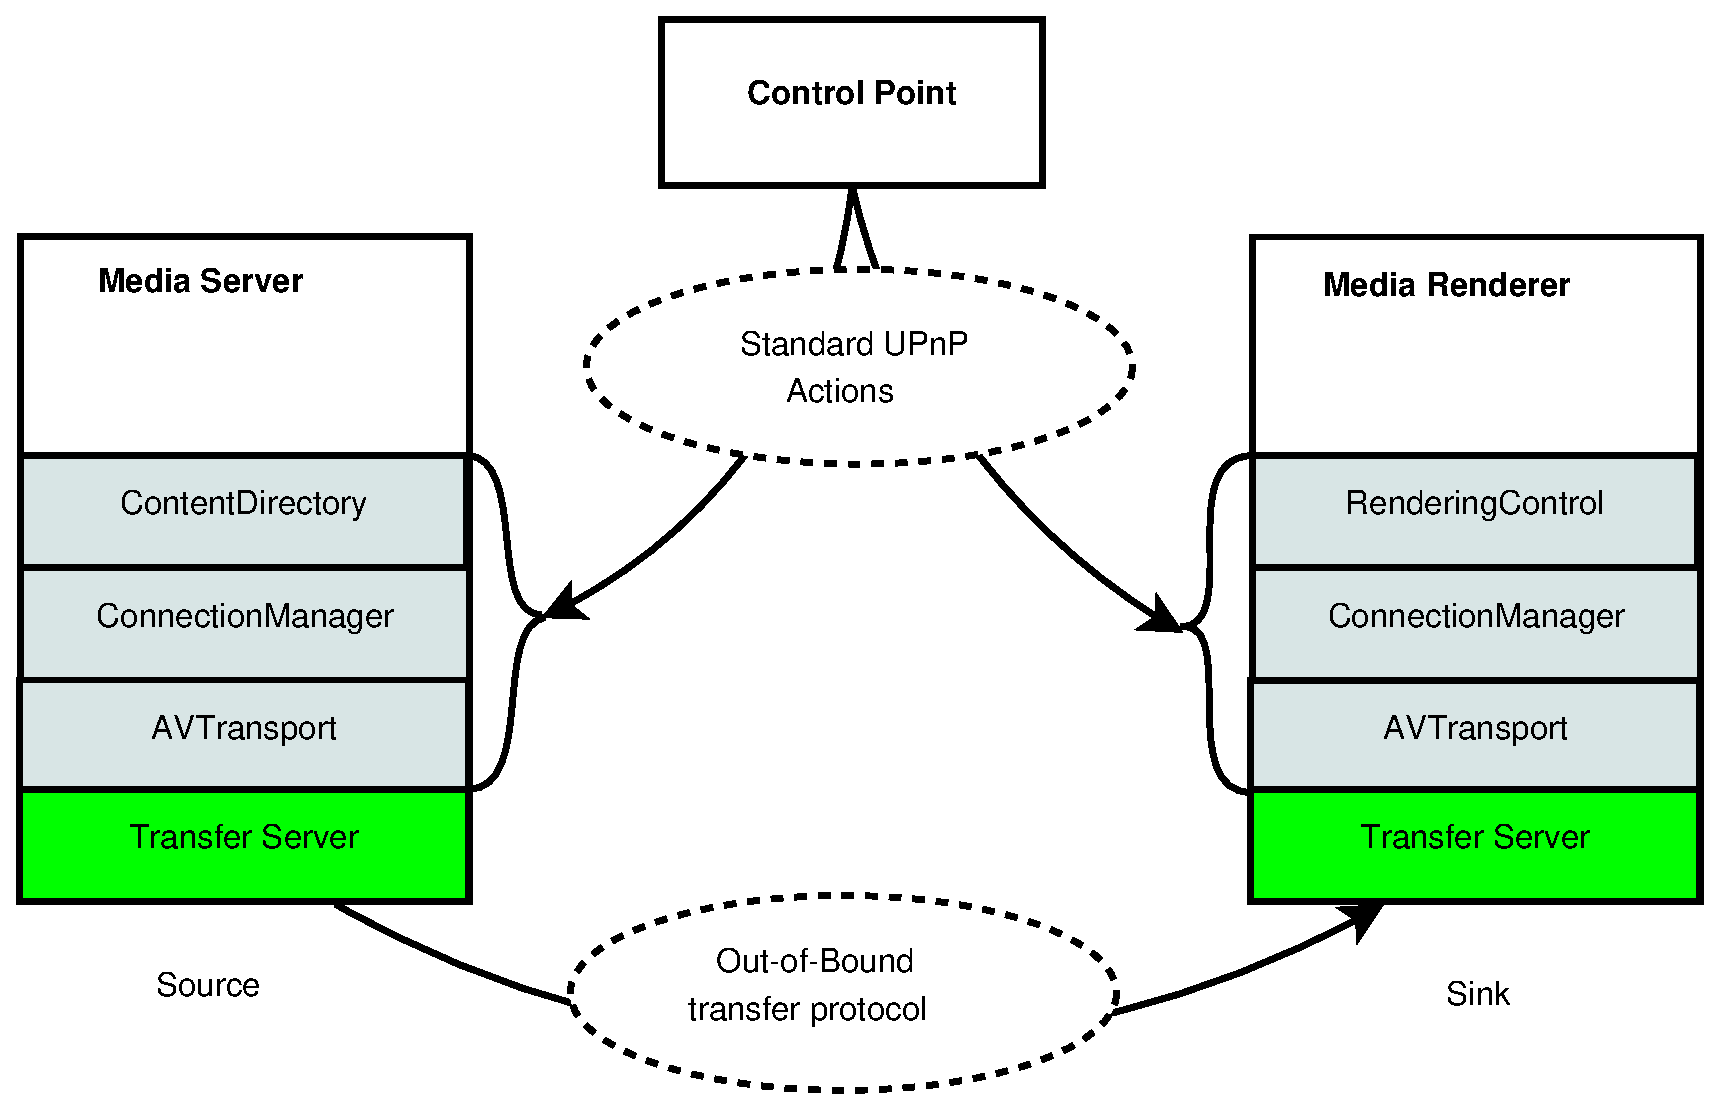
\includegraphics[height=9cm]{charts/upnp_playback} 
\caption{UPnP A/V playback architecture \label{upnp_playback}} 
\end{figure} 

\begin{enumerate} 
\item Media Server \\ 
The media server is used to locate available content in the home network. It's 
primary purpose is to allow control points to enumerate (browse or search) 
content items that are available for the user to render. The media server 
contains a ContentDirectory Service(CDS), a ConnectionManager Service(CM) 
, and an optional AVTransport Service(AVT) which depends on the supported 
transfer protocols. Some media servers are capable of transferring multiple 
content items at the same time. 

The ContentDirectory service is used by the control point to enumerate the content 
on the server. The primary action is ContentDirectroy::Browse(). After 
invoking this action, the control point can obtain detailed information of each 
item that the server can provide. This detailed information includes name, 
artist, date created, size and also the transfer protocols and data formats that 
supported by the for particular item. By parsing this detailed information, 
the control point is able to distinguish whether the item can be rendered by the 
given media renderer. 

The ConnectionManager service is used to manage the connections between a 
control point and a device. The primary action is 
ConnectionManager:: PrepareForConnection(), which is invoked by the control 
point to prepare the server for an upcoming transfer. This 
action will return the instanceID of an AVTransport service that will be used 
later to control, say to stop, pause, seek, the flow of content. The instanceID is used to distinguish multiple instances of the AVTransport service. Since each instance is associated with a particular connection to the renderer, the instanceID enables multiple renderer support at the same time. When the 
control point need to disconnect the connection, it will invoke the media 
server's ConnectionManager::ConnectionComplete() action to release the 
connection. When the ConnectionManager::PrepareForConnection() action is not 
implemented, the control point is only able to support a single renderer at a 
time. In this case 0 will be used as InstanceID. 

The AVTransport service is used by the control point to control the playback of the 
content. Operations like Stop, Pause, Seek are supported by this service. However, this 
service is not mandatory and the media server can choose to implement this feature 
according to the supported transfer protocols and data formats. If this service 
is supported, the InstanceID included in each AVTransport action is used to 
distinguish multiple instances of the service. New instances of the AVTransport 
service can be created by ConnectionManager's 
ConnectionManager::PrepareForConnection() action, and new InstanceID is 
allocated to each new service instance. 

\item Media Renderer \\ 
The media renderer is used to render the content obtained from home 
networking. Its main feature is that it can be discovered by a control point and perform content rendering according to the instructions from the control point. These instructions could control rendering settings such as brightness, contrast, volume, mute, etc. The control of flow of the content like stop, pause, seek can also be supported depending on the transfer protocol used. The media 
renderer provides three services including the RenderingControl service, the ConnectionManager 
service and an optional AVTransport service. Sometimes the rendering control and 
AVTransport services contain multiple independent instances so that the devices 
could be able to handle multiple content items at the same time. Those multiple 
instances can be identified by a unique InstanceID. 

The RenderingControl service is used by the control point to control how the renderer 
renders the incoming content. Characteristics like brightness, contrast, 
volume, mute etc, can be controlled by this service. The RenderingControl service 
supports multiple, dynamic instances, which allows a renderer to mix one or 
more items together. Such a dynamic instance could be a Picture-in-Picture window on a TV or a mixed audio stream. Multiple connections can be distinguished by their unique InstanceID. 

The ConnectionManager service is used to manage connections associated with a 
device, the primary action is the ConnectionManager::GetProtocolInfo() action. 
The control point can invoke this action to enumerate the transfer protocols and 
data formats supported by the media renderer. By comparing this information with 
the protocol information retrieved from the media server, the control point is able to 
predetermine if a media server is capable of rendering a specific item from 
the media server. Optionally, media renderer may also implement the
ConnectionManager::PrepareForConnection() action to prepare itself for an 
upcoming transfer. It can also assign a unique ConnectionID that can be used by 
a 3rd party control point to obtain information about the connections that media 
renderer is using. In addition, depending on the transfer protocol and data 
format used, this action may also return a unique AVTransport InstanceID that the control 
point can use to control the flow of content(stop, pause, seek, etc). 

The AVTransport service is used to control the flow of streamed content. Actions 
like play, stop, pause and seek can be controlled depending on the transfer 
protocol and supported data formats. The AVTransport service can also support 
multiple logical instances and handle multiple simultaneous content items. The 
AVTransport InstanceID which is used to distinguish service instances can be 
allocated by ConnectionManager::PrepareForConnection(). 

\item Control Point \\ 
The Control Point is used to bridge communication between a media server and a media renderer. 
It also provides the user interface to users. A control point does not implement UPnP 
services, as a result it is not visible as a device on the network. Usually the control point 
invokes a media server or a media renderer's services in order to complete the 
desired operations.

The user control point can be used in different scenarios and usually it can 
perform the following functions: 

\begin{itemize} 
\item Discover A/V devices 
\item Locate desired media content 
\item Get renderer's supported protocol and formats 
\item Compare and match protocols and formats between media server and media 
renderer 
\item Configure media server and media renderer 
\item Select desired content 
\item Start content transfer between media server and media renderer 
\item Adjust rendering characteristics 
\item Select next content in the list 
\item Cleanup media server and media renderer 
\end{itemize} 

\end{enumerate} 

As described above, three basic functional entities are defined in the UPnP AV 
architecture\cite{upnp-av}, which are Media Server, Media Renderer and Control Point respectively.
A physical device can consist of a combination of any of these functional 
entities. One typical example is that a DLNA Media player is a combination of a Control 
Point and a Media renderer. \\
\\
A simplified UPnP Audio Video 3-box model \cite{DLNA_proxy} can be 
seen as below: 

\begin{figure}[htb] 
\centering 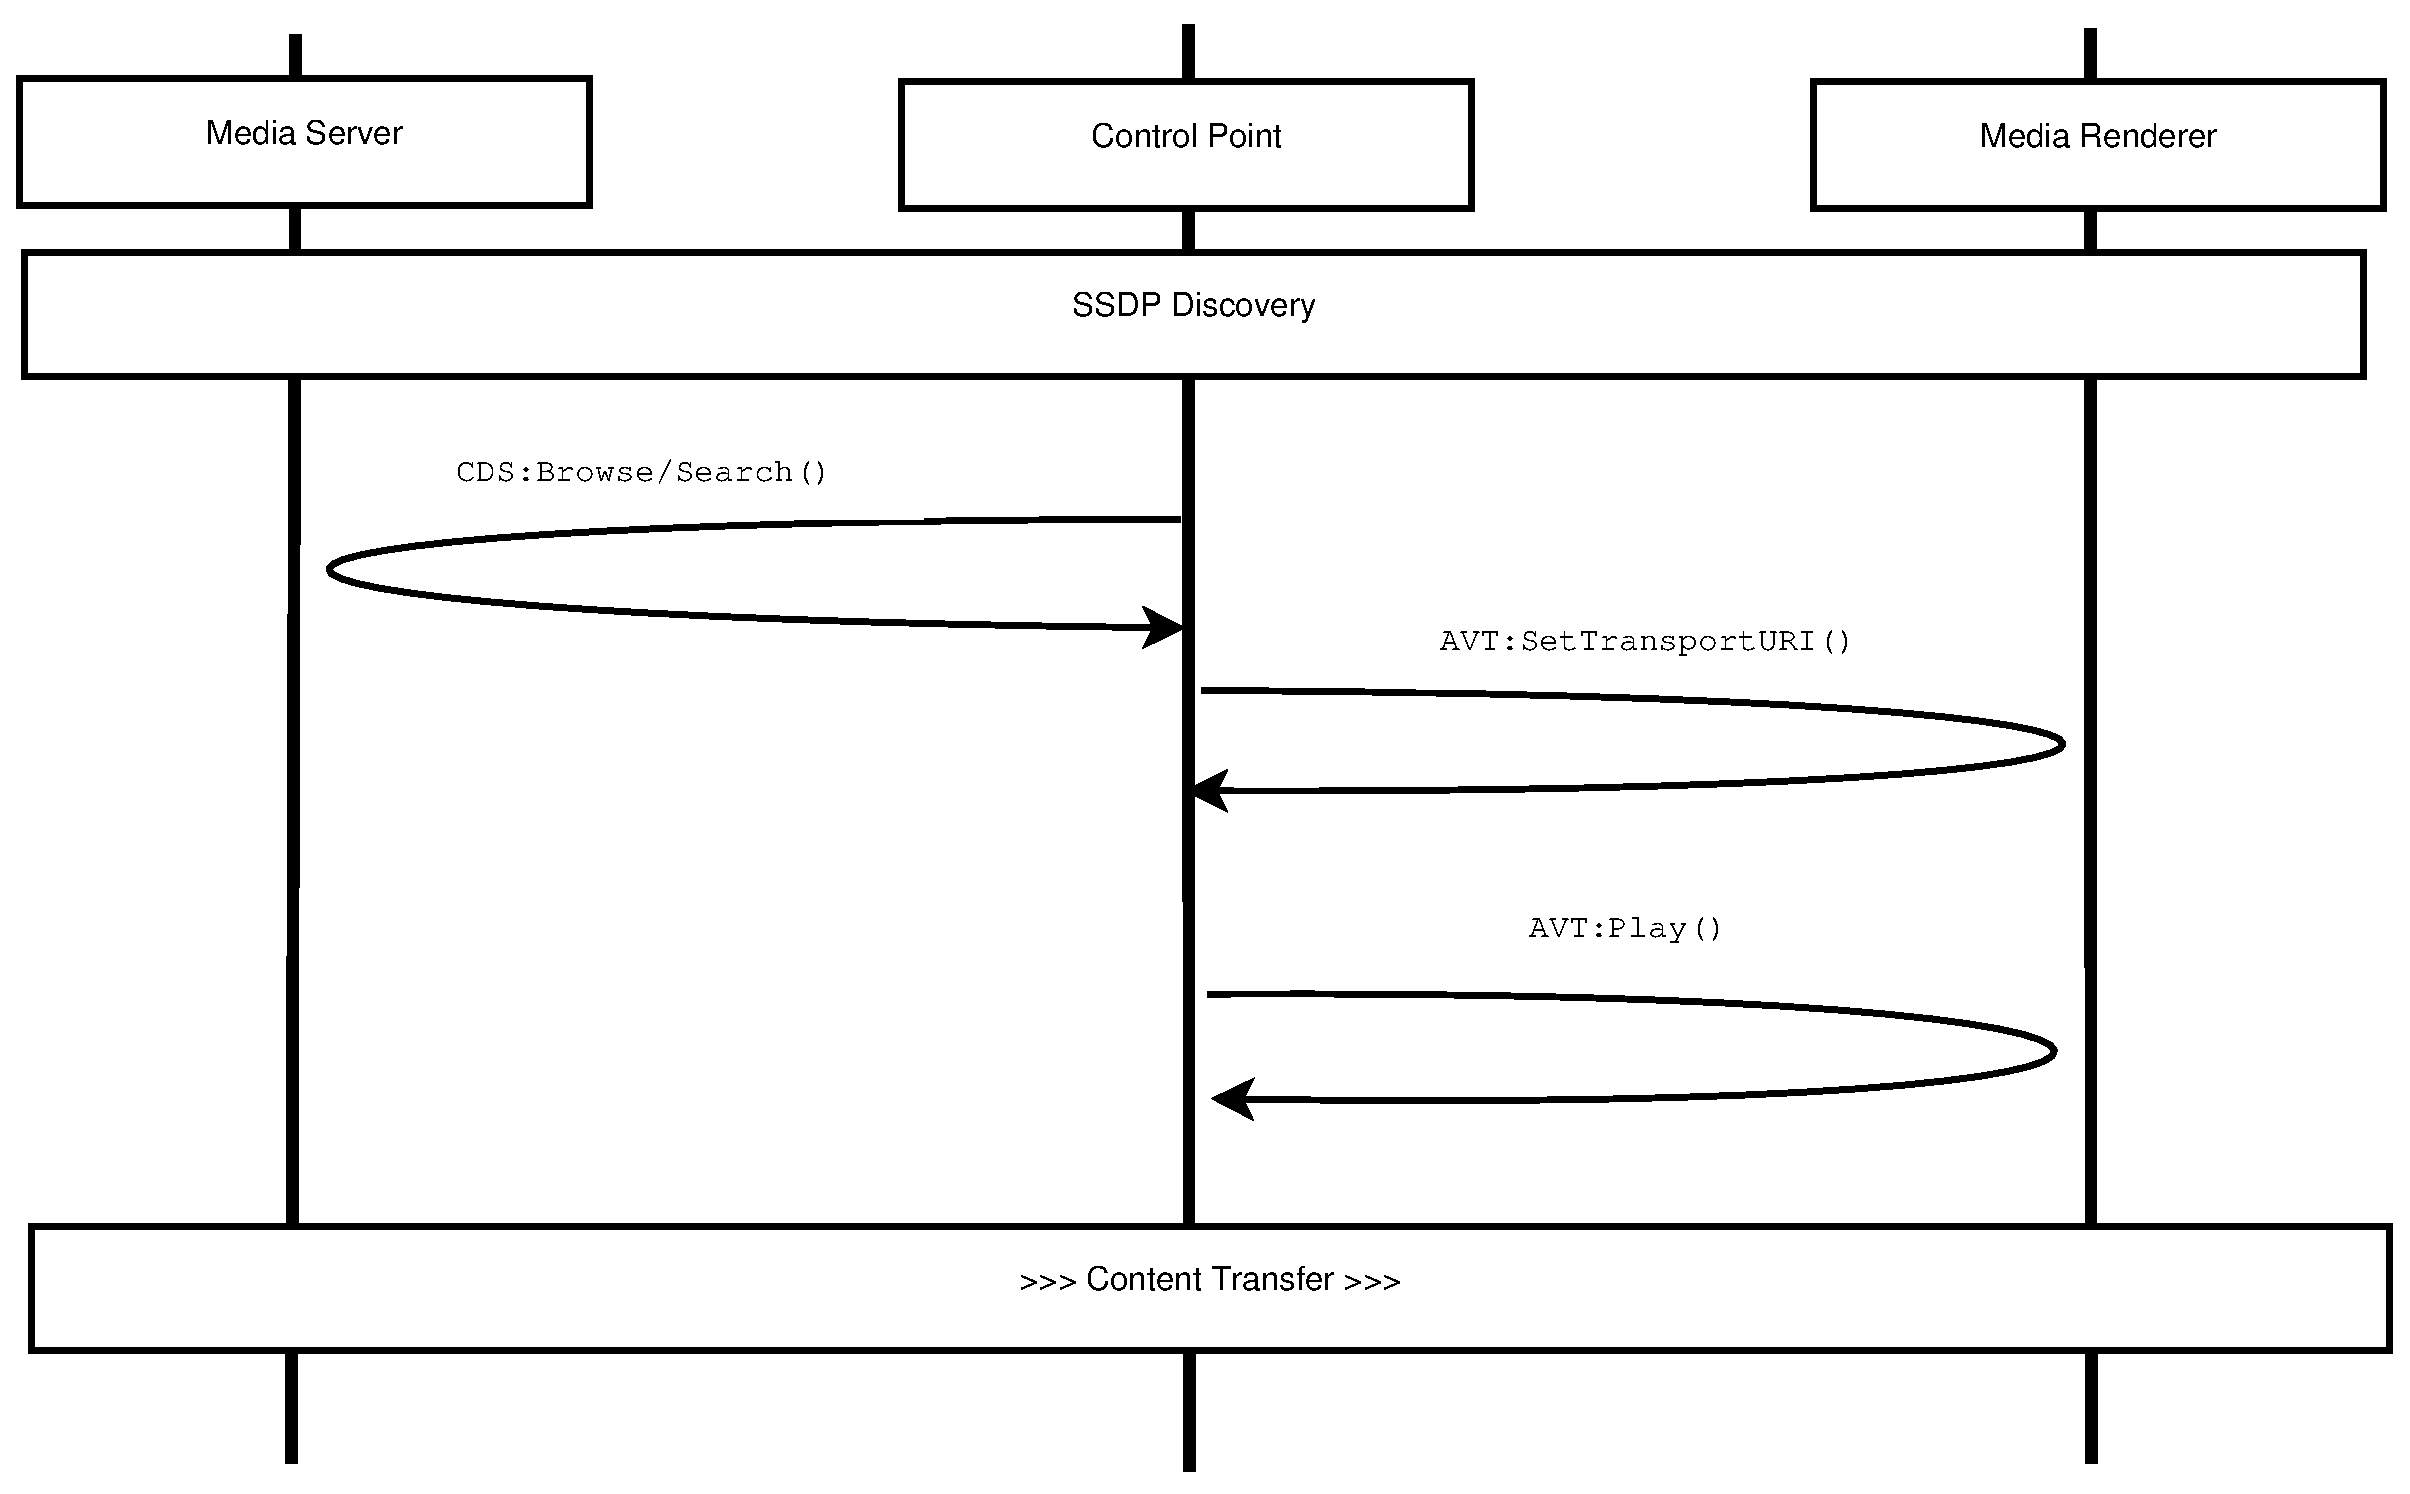
\includegraphics[height=9cm]{charts/chart1} 
\caption{Typical UPnP AV use scenario \label{chart1}} 
\end{figure} 

The first thing in UPnP network communication is the Simple Service Discovery 
Protocol(SSDP)-based device discovery. A SSDP multicast message is sent when a 
new device is added to the network. A control point would listen to these 
multicast messages. On receiving the SSDP message, the control point would send a request for the device's description and services using the location found in the SSDP discovery message. Then the control point can issue the services action command using the Simple Object Access protocol (SOAP).\\
\\ 
In media sharing scenarios, the control point would browse the information about 
the Content Directory Service (CDS) provided by the Media Server. A 
browse/Search action can be invoked to navigate through the content stored in 
the Media Server device. After the control point has selected the media content from 
Media Server, a Media Renderer AVTransport::SetAVTransportURI would be sent by 
the control point to the Media Renderer. Finally, the Play command is invoked by 
the control point to instruct the Media Renderer. Afterward, the transfer begins. The media 
stream travels directly between the Media Server and the Media Renderer, through HTTP, 
RTP or other streaming protocols. \\
\\
The media playback control actions can also be invoked by the control point. Methods 
supported include volume control, seek, pause etc. 

\subsubsection[DLNA]{DLNA\footnote{Digital Living Network Alliance}} 
DLNA is a relatively old industry standard compared with other home networking 
solutions. It is mainly based on the UPnP Audio/Video architecture, which is 
discussed in \ref{upnp}. As a result it is widely used by many manufactures. Newer 
home networking solutions are also influenced by DLNA and they follow similar 
technologies used in DLNA. In this paper the DLNA and UPnP standard architectures are studied to help us gain a grasp of how a home networking solution could look like. \\
\\
An overview of the DLNA architecture \cite{dlna_guideline} is described below: 
\begin{enumerate} 
\item Architectures and Protocols 

%% table 3, Key Technology Ingredients 
\begin{table}[htb] 
\caption{Key Technology Ingredients \label{Table3}} 
\begin{center} 
\fbox{ 
\begin{tabular}{c|c}  
\textbf { Functional Components } & { Technology Ingredients } \\ \hline 
\textbf Connectivity & Ethernet, 802.11 (including Wi-Fi Direct) \\ 
\textbf  & MoCA, HPNA and Bluetooth \\ \hline 
\textbf Networking & IPv4 Suite \\ \hline 
\textbf Device Discovery and Control & UPnP* Device Architecture v1.0 
\ref{upnpdevice} \\ \hline 
\textbf Media Management and Control & UPnP AV and UPnP Printer:1 
\ref{upnpav}\\ \hline 
\textbf Media Formats & Required and Optional Format Profiles \\ \hline 
\textbf Media Transport & Media Transport \\ \hline 
\textbf Remote User Interfaces & CEA-2014-A 
\end{tabular} 
} 
\end{center} 
\end{table} 

The DLNA architecture is built upon the UPnP protocol, which is discussed in 
 in \ref{upnp}. 
In the network layer DLNA uses the IPv4 suite. On top of the network layer, the UPnP device architecture and UPnP AV architecture is used to control and manage media devices. The DLNA 
guideline also addresses the media format compatibility and media transport 
interoperability issues in support of interoperability among devices. 

\item Media Format Profiles \\ 
DLNA defines the media formats used by the DLNA home networking 
standard. There are three types of media in DLNA: music, video and photo. 
\begin{enumerate} 
\item Music \\ 
Minimal requirement is the LPCM format. Used by PCM raw data, this format is not compressed and it does not require heavy CPU usage. However the bandwidth consumption is 
considerably bigger than other formats. 

MP3 is the most popular music format. It is a compressed format and requires 
some CPU power for encoding or decoding. Compared with LPCM, the bandwidth consumption of MP3 is less, making it suitable for low bandwidth networking. 

AAC is another kind of compressed audio format and it becomes popular since it is the default media format of iTunes. It has similar characteristics of MP3. 
\item Photo \\ 
The minimal requirement in the DLNA guideline is the JPEG format. In many occasions JPEG is the only suggested format due to its proven quality and compress ratio. 
\item Video \\ 
The minimal requirement in DLNA guideline is the MP4 format. The detailed audio and video codecs are also specified in DLNA media format guidelines. 
\end{enumerate} 
In a device-to-device scenario, the media server may store a huge amount of differently 
formatted media. The communication between two devices should follow the same encoding mechanism. Normally the media server takes the responsibility to transcode the media to a certain format defined by the DLNA media format profile guideline. 
\item Link Protection \\ 
DLNA Link Protection is defined as the protection of a content stream between two 
devices on a DLNA network against illegitimate observation or interception. 

Content protection is an important mechanism to ensure that commercial content is protected 
from piracy and illegitimate redistribution. Link Protection is a technique that enables 
distribution of protected commercial content on a home network. It provides protection for copyright holders and content providers without sacrificing consumer flexibility. 
\item Digital rights management (DRM) Interoperability Solutions (DIS) \\ 
DIS is intended to be used to enable the secure transfer and use of protected 
commercial content among different implementations on network media devices. 
The content could be protected by different content protection technologies, 
which are described as DRMs in short. 
\item Device Profiles \\ 
A Device Profile is a collection of DLNA capabilities and features within a DLNA device. For a device 
to be compliant with a Device Profile, it has to conform to all of the guidelines listed for that 
Device Profile. 

In practice, Device Profiles reference existing optional or recommended DLNA guidelines that enable certain features, and makes those DLNA guidelines mandatory within the context of a Device Profile. 
A Device Profile can also provide some additional guidelines that complement or modify existing DLNA guidelines for a feature. 

A particular type of DLNA Device Profile is the Commercial Video Profile (CVP). A CVP Device Profile is an extension of the DLNA guidelines that will allow content from service providers and multichannel video programming distributers to be distributed on the DLNA network. DLNA Commercial Video Profiles (CVPs) are defined as Device Profiles that consistently enable commercial content that enters the home network through a gateway device via an interface to a commercial content service provider. Since different regions of the world have different requirements for commercial content, there are multiple CVPs defined. 

\end{enumerate} 

\subsubsection{AirPlay} 
AirPlay is Apple Inc's home networking solution. It is a family of protocols 
used to display different types of media content on Apple TV from other iOS devices. 
AirPlay support multiple functions, including displaying photos and sideshows from iOS devices, streaming audio from iOS devices or iTunes, as well as displaying videos from iOS device and 
showing the whole screen on Apple TV, which is known as AirPlay Mirroring. \\
\\
AirPlay's specification is not open to public. However unofficial specifications have been made by some hackers through reverse engineering the protocol stack \cite{AirPlay-spec}. These unofficial specifications could be found on the Internet \cite{AirPlay-spec}.  
The specification includes 6 parts, which are described below: 

\begin{enumerate} 
\item Service Discovery \\ 
The service discovery of AirPlay stems from the IETF Zeroconf Working Group, 
who is dedicated to improve the ease-of-use (Zero Configuration) of networks. The 
Zeroconf working group has made it possible to make two devices in the 
network to communicate effectively using IP, without requiring a specialist to manually 
configure the network. 

AirPlay's service discovery is based on Multicast DNS \cite{multicastdns}, which 
fulfills the Zeroconf requirement. Multicast DNS is a way of using familiar DNS 
programming interfaces, packet formats and operating semantics, in a small 
network where no conventional DNS server has been installed. The requirements 
for Zeroconf name resolution could be met by designing an entirely new 
protocol, since it is better to provide this functionality by making minimal changes 
to the current standard DNS protocol. By using Multicast DNS, most current 
applications need no changes at all to work correctly using mDNS in a Zeroconf network. Besides,
engineers do not have to learn an entirely new protocol. Moreover current network 
packet capture tools are already capable of  decoding and displaying the DNS packets. Thus they do not 
have to be updated to understand new packet formats. 

An AirPlay device such as the Apple TV publishes two services. The first one is 
RAOP (Remote Audio Output Protocol), used for audio streaming. The second 
one is the AirPlay service, used for photos and video content. 

The AirPlay server is an HTTP server (RFC 2616). Two connections are made to this 
server, with the second one being used as a reverse HTTP connection. This allows a 
client to receive asynchronous events, such as playback status changes, from a 
server. 
\item Video streaming \\ 
The video streaming uses typical HTTP streaming technology, the controller sets 
the streaming URL to Apple TV or other AirPlay receivers. While the URL is set, 
Apple TV starts to download video from the server using the URL and starts 
playing when enough data is buffered. The control messages can be seen in 
table \ref{video_stream}. 

Note that Apple TV does not support Video Volume Control. 
%% table , Video Streaming 
\begin{table}[htb] 
\caption{AirPlay Video Control HTTP requests \label{video_stream}} 
\begin{center} 
\fbox{ 
\begin{tabular}{c|l|l}  
\textbf { Method } & { Request } & { Description }\\ \hline 
\textbf GET & /server-info & Fetch general informations about the AirPlay server \\ \hline 
\textbf POST & /play & Start video playback \\ \hline 
\textbf POST & /scrub & Seek at an arbitrary location in the video \\ \hline 
\textbf POST & /rate & Change the playback rate,0 is paused, 1 is normal \\ 
\hline 
\textbf POST & /stop & Stop playback \\ \hline 
\textbf GET & /scrub & Retrieve the current playback position \\ \hline 
\textbf GET & /playback-info & Retrieve playback informations like position, 
duration\ldots \\ \hline 
\textbf PUT & /setProperty & Set playback property \\ \hline 
\textbf GET & /getProperty & Get playback property 
\end{tabular} 
} 
\end{center} 
\end{table} 
\item Photo streaming \\ 
Image streaming uses the HTTP put message to send raw image data to Apple TV or 
other devices. After the whole image is received, the image is then rendered on 
screen. AirPlay also supports slide show, the control message can be seen in 
table \ref{photo_stream}. 
\begin{table}[htb] 
\caption{AirPlay Photo Control HTTP requests \label{photo_stream}} 
\begin{center} 
\fbox{ 
\begin{tabular}{c|l|l}  
\textbf { Method } & { Request } & { Description }\\ \hline 
\textbf GET & /slideshow-features & Fetch the list of available transitions for slideshows \\ \hline 
\textbf PUT & /photo & Send a JPEG picture to the server \\ \hline 
\textbf PUT & /slideshows/1 & Start or stop a slideshow session \\ 
\hline 
\textbf POST & /stop & Stop a photo or slideshow session 
\end{tabular} 
} 
\end{center} 
\end{table} 
\item Music streaming \\ 
AirPlay music streaming is a bit different from video and image streaming. The 
technology used is the RTSP streaming protocol, which is more of a "push like" protocol. Different than HTTP streaming where the server responds a request, The RTSP streaming server actively pushes UDP packets to the receiver . However Apple does not use the standard RTSP but instead uses its own implementation of RTSP, which is called RAOP (Remote 
Audio Output Protocol). The control messages of RAOP can be seen in table 
\ref{music_stream}. 
\begin{table}[htb] 
\caption{AirPlay Audio Control RTSP requests \label{music_stream}} 
\begin{center} 
\fbox{ 
\begin{tabular}{c|l}  
\textbf { RTSP request } & { Description }\\ \hline 
\textbf OPTIONS & Ask the RTSP server for its supported methods \\ \hline 
\textbf ANNOUNCE & Tell the RTSP server about stream properties using SDP \\ 
\hline 
\textbf SETUP & Initialize a record session \\ \hline 
\textbf RECORD & Start the audio streaming \\ \hline 
\textbf FLUSH & Stop the streaming \\ \hline 
\textbf TEARDOWN & End the RTSP session 
\end{tabular} 
} 
\end{center} 
\end{table} 

\item Screen mirroring \\ 
AirPlay screen mirroring is achieved by transmitting H.264 encoded video stream 
over a TCP connection. The stream is packeted with a 128-byte header. The 
audio uses the the AAC-ELD format and is sent using AirTunes protocol. 
The NTP(Network time protocol) protocol is used for synchronization and the synchronization 
takes place on UDP port 7010(client) and 7011(server). The 
AirPlay server runs a NTP client. Requests are sent to an AirPlay client every 3 
seconds. The reference time stamp marks the beginning of the 
mirroring session.  The control messages can be seen in table 
\ref{mirroring_stream}. 
\begin{table}[htb] 
\caption{AirPlay Mirroring Control HTTP requests \label{mirroring_stream}} 
\begin{center} 
\fbox{ 
\begin{tabular}{c|l|l}  
\textbf { Method } & { Request } & { Description }\\ \hline 
\textbf GET & /stream.xml & Retrieve information about the server capabilities 
\\ \hline 
\textbf POST & /stream & Start the live video transmission 
\end{tabular} 
} 
\end{center} 
\end{table} 
\item Authentication \\ 
An AirPlay server can require a password for displaying any content from the 
network. It is implemented using standard HTTP Digest Authentication (RFC 2617), 
over RTSP for AirTunes, and HTTP for everything else. The digest realms and 
usernames accepted by Apple TV are described in table \ref{hda}. 
%% table , AirPlay Authentication 
\begin{table}[htb] 
\caption{AirPlay HTTP Digest Authentication \label{hda}} 
\begin{center} 
\fbox{ 
\begin{tabular}{c|c|c}  
\textbf { Service } & { Realm } & { Username }\\ \hline 
\textbf AirTunes & roap & iTunes \\ \hline 
\textbf AirPlay & AirPlay & AirPlay 
\end{tabular} 
} 
\end{center} 
\end{table} 
\end{enumerate} 

\subsubsection{DIAL} 
Chromecast and FireTV use the DIAL \cite{dial} (DIscovery And Launch) protocol,
co-developed by Netflix and YouTube, to search for available devices on a Wi-Fi network. 
Once a device is discovered, the protocol synchronizes information on how to 
connect to the device. The protocol is proposed by Google and Netflix and consequently 
YouTube and Netflix  have already had their build in DIAL device discovery functionality. The 
streaming part uses HTTP streaming, which means a controller can directly set the 
streaming URL and the receiver will start downloading automatically. \\
\\
The DIAL protocol has two components: DIAL Service Discovery and the DIAL 
Representational State Transfer (REST) Service. DIAL Service Discovery enables a 
DIAL client device to discover DIAL servers on its local network and gain access to the DIAL REST Service on those devices. The DIAL REST Service enables a DIAL client to query, launch, and optionally stop applications on a DIAL server device. 
\begin{enumerate} 
\item DIAL Service Discovery \\ 
The DIAL Service Discovery protocol is based on Simple Service Discovery 
Protocol (SSDP), which is defined as part of UPnP device architecture discussed 
in \ref{upnp}. 

A DIAL client will first send an M-Search request, which includes  the Search Target 
header, over UDP to the IPv4 multicast address 239.255.255.250 and UDP port 1900. After that the SSDP/UPnP server responds with a response message including a LOCATION header 
containing an absolute HTTP URL for the UPnP description of the root device. 
When receiving the M-SEARCH response, the DIAL client then sends an HTTP GET 
request to the URL found in the LOCATION header of the M-SEARCH response, to 
get a prospected HTTP response message containing a XML format UPnP device description. The 
overall flow of DIAL discovery is shown in figure \ref{dial_discovery}. 

\begin{figure}[htb] \centering 
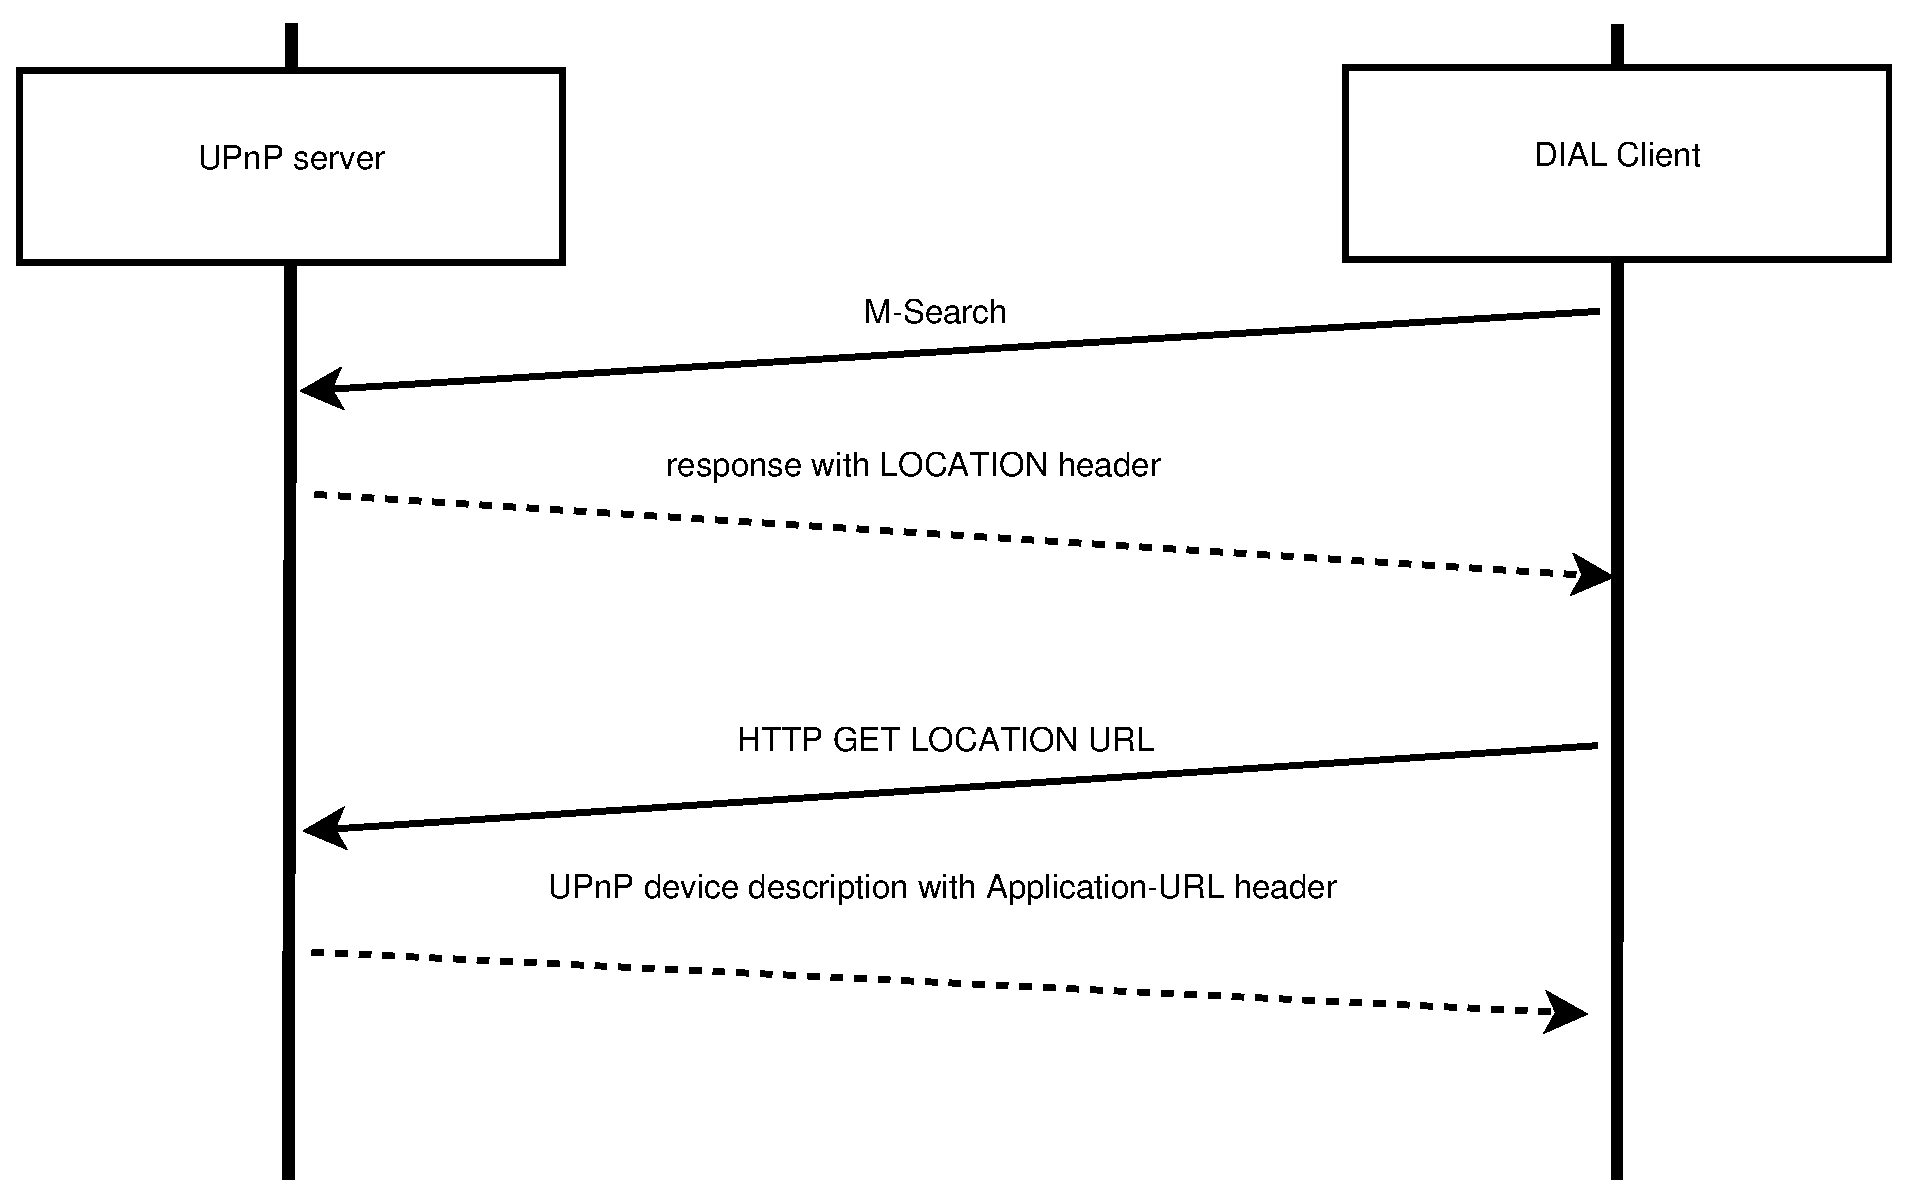
\includegraphics[height=9cm]{charts/dial_discovery} 
\caption{DIAL Discovery \label{dial_discovery}} 
\end{figure} 

\item DIAL REST Service \\ 
The DIAL REST service allocates URLs for different resource applications such as 
YouTube and Netflix. Then the application can be controlled by issuing HTTP 
requests against the URL for that application. The Application resource URL is 
constructed by concatenating the DIAL REST service URL, a single slash character 
('/') and the application name. The application name must be registered in DIAL 
Registry to be used. 

A DIAL client sends an HTTP GET request to the application resource URL. 
The server receiving the request then extract the application name and check if the 
application is installed or not. If the application is not recognized, the 
server will either return 404 Not Found or trigger the installation of this specific 
application. If the application has been installed, the DIAL server return 
an HTTP response with 200 OK and a body contains MIME type in XML. 

The client then sends a HTTP POST request to the application resource URL to 
launch the desired application. On receipt of a valid POST request, the DIAL 
server will extract the application name, run the application, and then send 
a HTTP response with the LOCATION header, to inform the absolute HTTP URL, which 
identifies the running instance of the application. 

The first-screen application can also send small amount of data to the DIAL 
server, and then DIAL server can send the information to DIAL clients. 
After the application is launched and communication is established, the DIAL 
client can communicate directly with the application. The flow chart of  the DIAL REST service is  shown as figure \ref{dial_rest}. 

\begin{figure}[htb] \centering 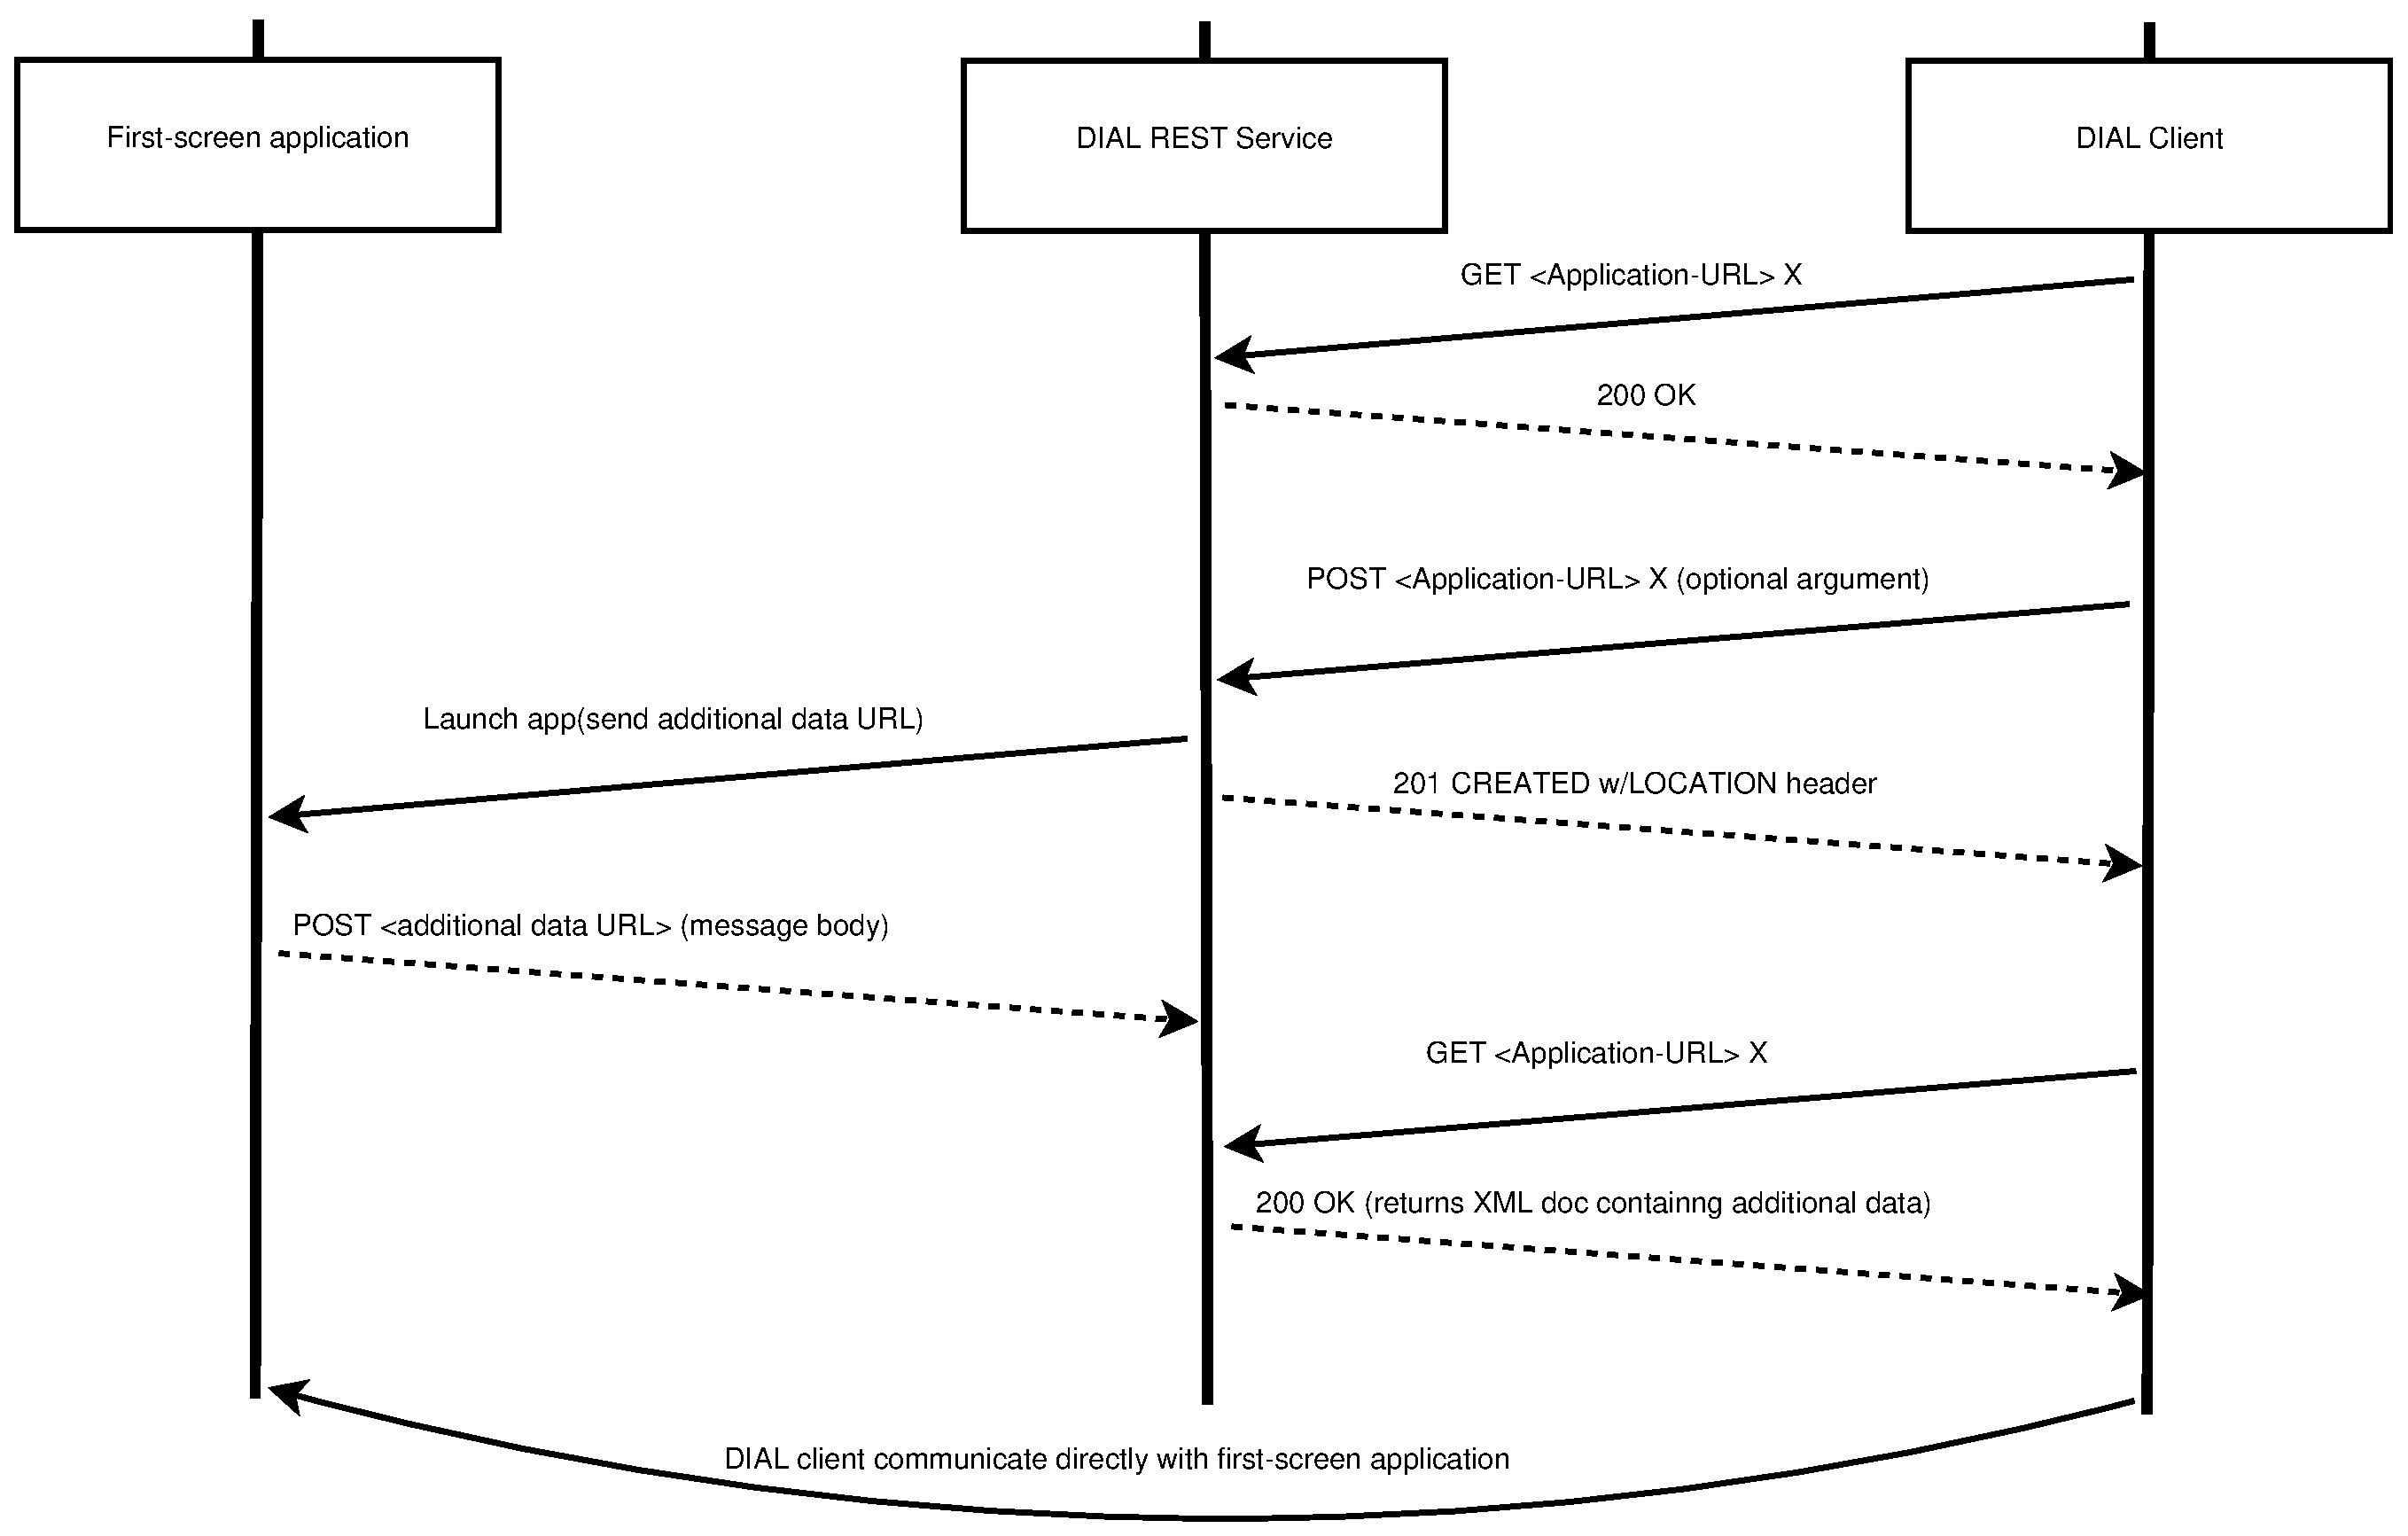
\includegraphics[height=9cm]{charts/dial_rest} 
\caption{DIAL REST service: application launch \label{dial_rest}} 
\end{figure} 
\end{enumerate} 

\subsubsection{Miracast} %NOT Edited

Miracast \cite{miracast_industry} is very different on technology perspective.
Devices which utilizing Miracast technology are not necessarily connected to
the same local network, Wi-Fi peer to peer connection will be created when
needed. This makes Miracast more adaptive than other technologies, in other
words, Miracast is not limited to the pre-configured network infrastructure.\\
\\
Another point worth mentioning is that Miracast utilizes many Wi-Fi alliance
building blocks that is constantly developed over the years. These components
include Wi-Fi CERTIFIED n (improved throughput and coverage), Wi-Fi Direct
(device-to- device connectivity), Wi-Fi Protected Access 2 (WPA2) (security),
Wi-Fi Multimedia (WMM) (traffic management) and Wi-Fi Protected Setup. These
technologies have enriched the user experience and increased user's trust in
Wi-Fi.\\
\\
Not limited to Wi-Fi direct connection, some Miracast devices also support Tunneled Direct Link Setup (TDLS), which allows devices to connect via an infrastructure network. TDLS enables more efficient data transfer and keeps the advantage of more advanced Wi-Fi capabilities at the same time.\\
\\
In most cases, Miracast connections are expected to be predominantly established between Wi-Fi devices connected with each other directly, without an AP acting as an intermediary. When two devices connect with each other directly, one fulfills its role as the source(the transmitting device) and the other functions as a display(the device receiving and rendering the content to the user).\\
\\
There are 4 typical topologies that are supported by Miracast. The  Source could directly connect to Display without AP present, or the Source with access to AP and direct connect to Display, or the source could directly connect to Display with AP present, but not connected, or the Source and Display could connect to each other and connect to AP at the same time. These four topologies can be described as in Figure  \ref{miracast_model}.

\begin{figure}[htb] \centering 
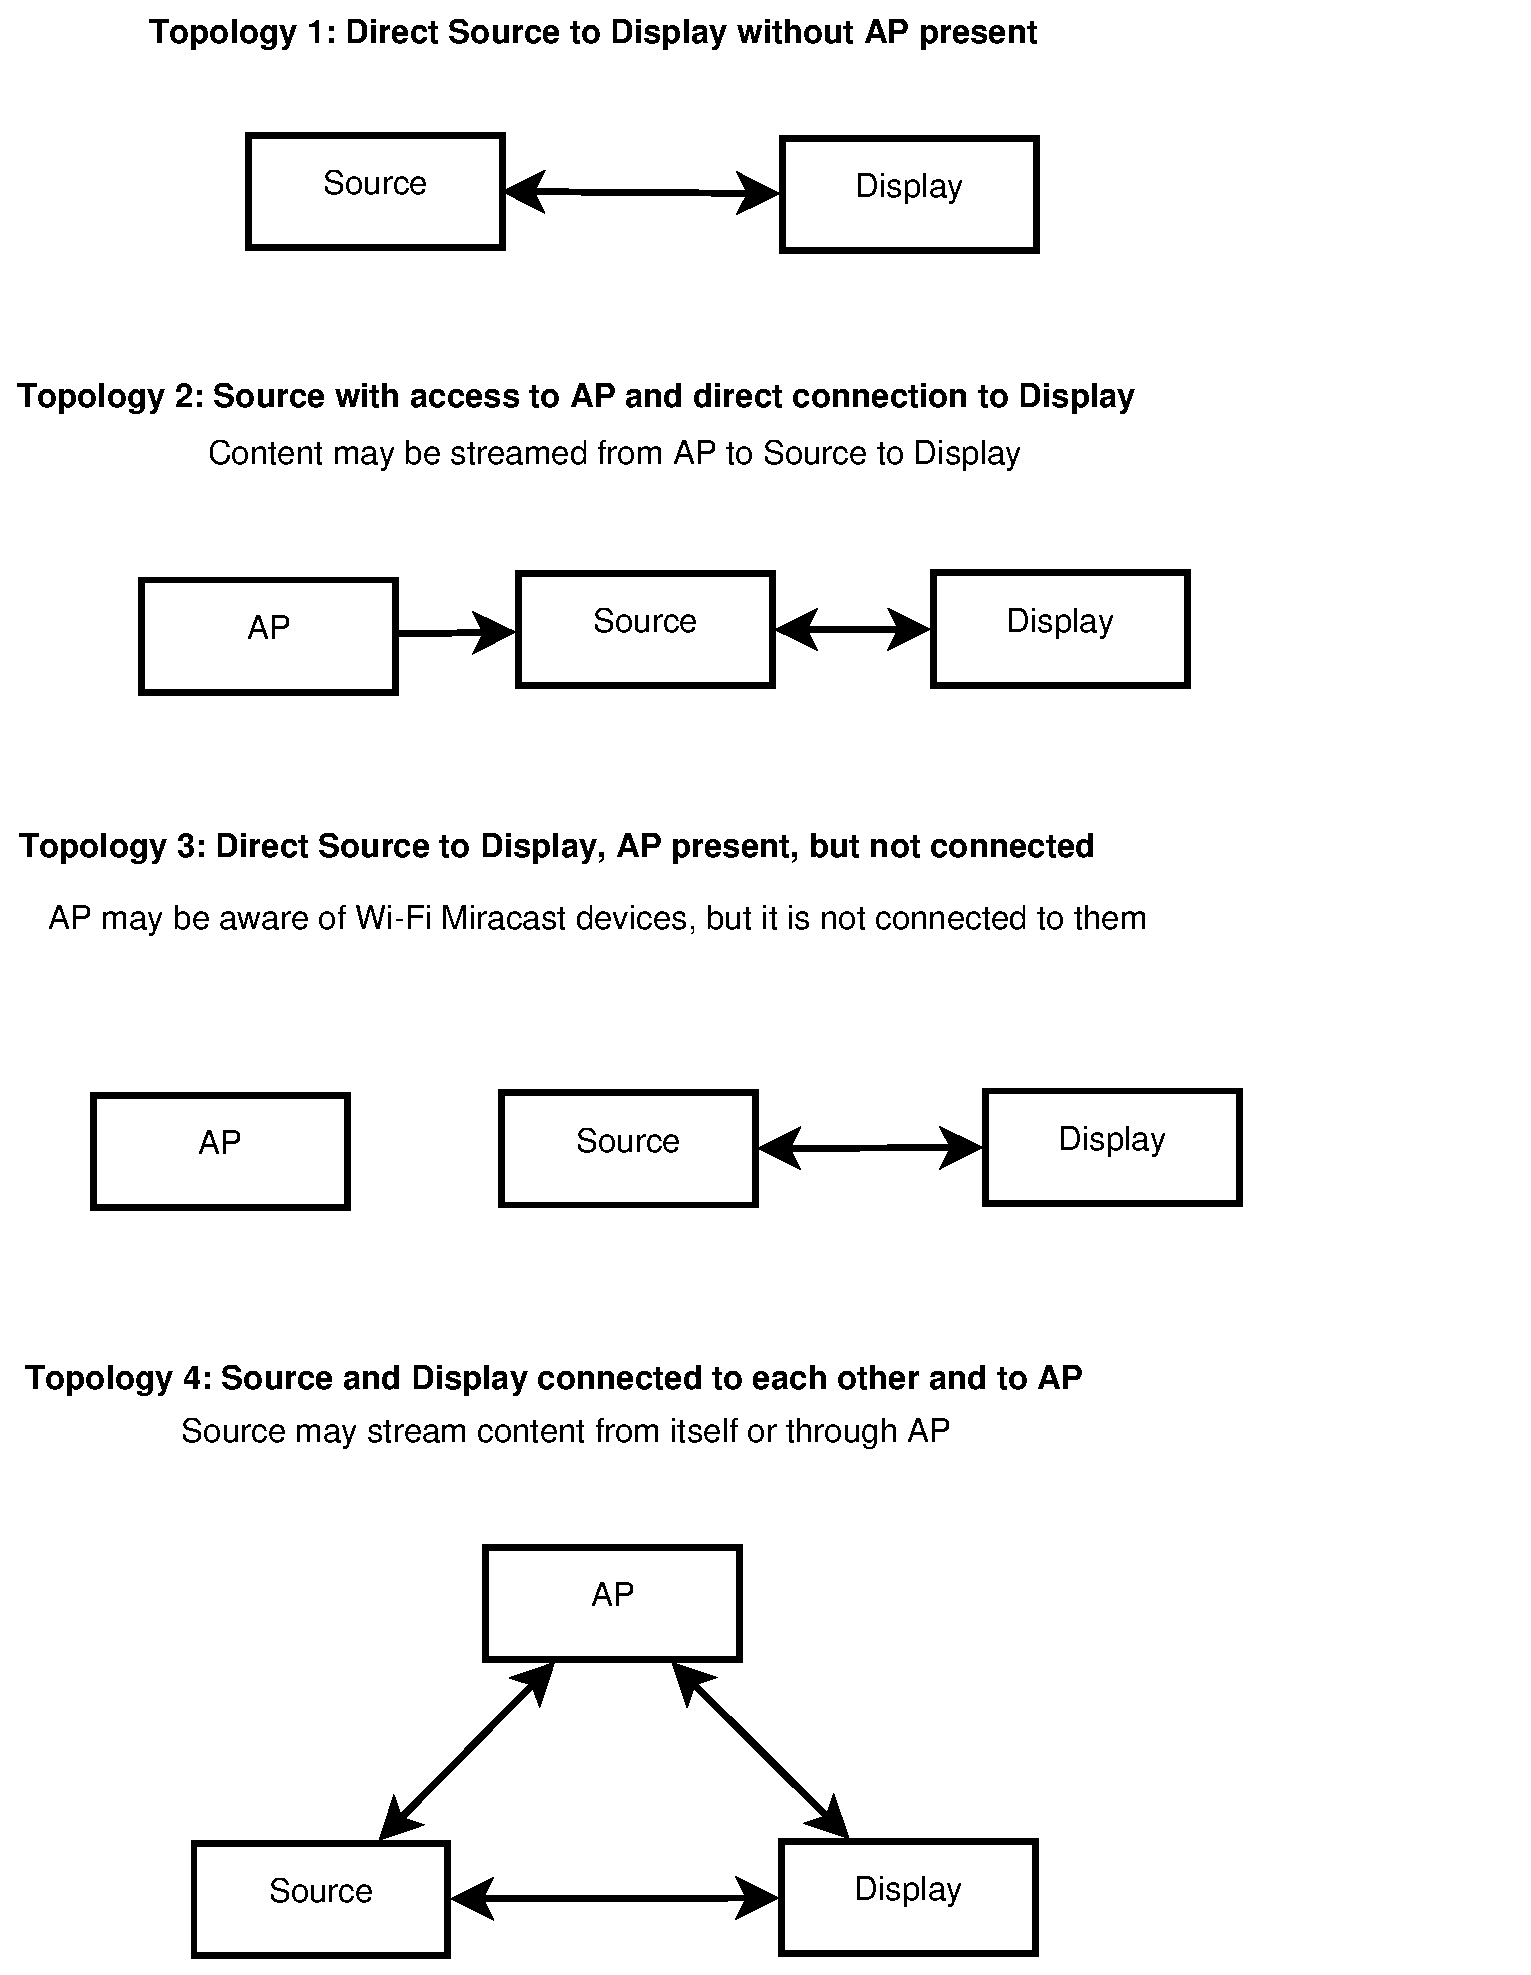
\includegraphics[height=14cm]{charts/miracast_model} 
\caption{Miracast topologies \label{miracast_model}} 
\end{figure} 

On technology perspective, as mentioned previously, Miracast is built upon many different Wi-Fi technologies. These technologies are built together in an architecture that can be described by Figure \ref{miracast_architect}. 

\begin{figure}[htb] \centering 
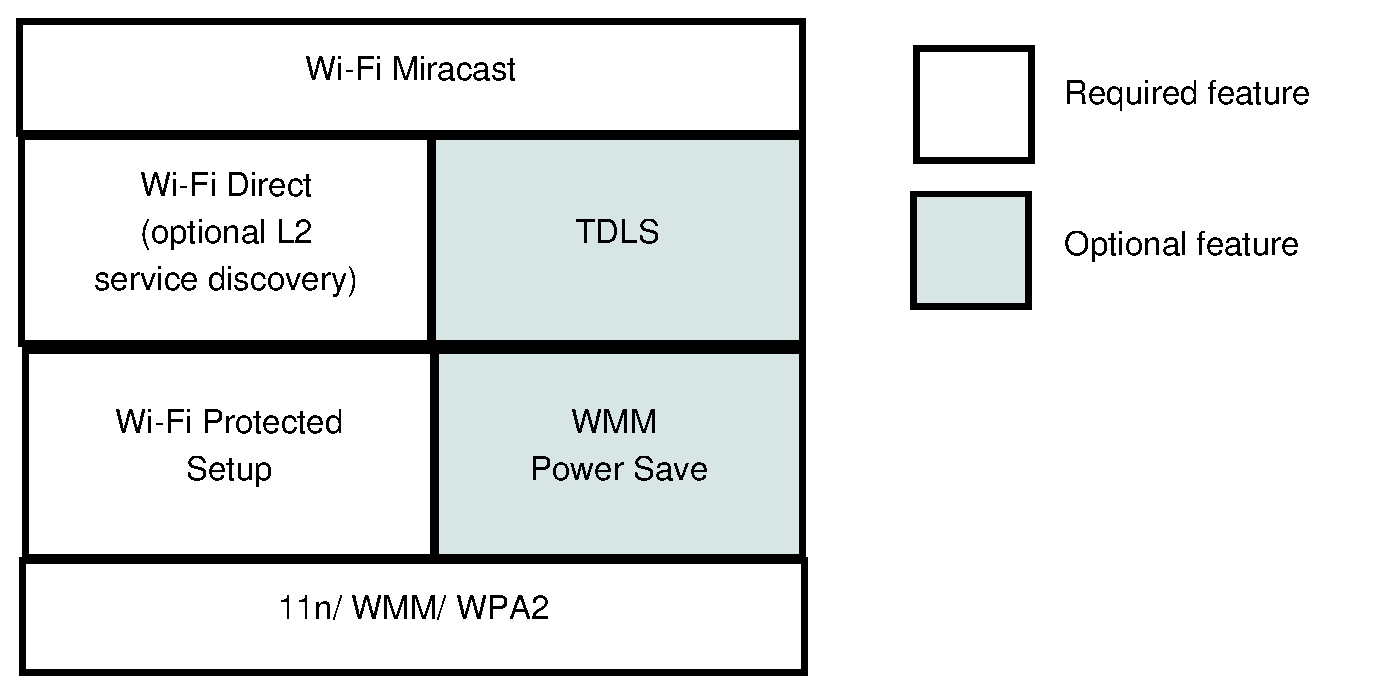
\includegraphics[height=5cm]{charts/miracast_technology_architecture} 
\caption{Miracast technology architecture \label{miracast_architect}} 
\end{figure} 

The technology component can be described in 6 different aspects: \\
\begin{enumerate} 
\item Connectivity\\ 
Wi-Fi CERTIFIED n provides a transmission channel designed to support 
multimedia content. 
\item Device-to-device connectivity\\ 
Wi-Fi Direct allows devices to connect directly to each other easily, without the need for a Wi-Fi AP. TDLS allows devices that are associated to the same Wi-Fi network to establish a direct 
link with each other. 
\item Security\\ 
WPA2 encrypts the transportation between the source and the display, ensures the safety of multimedia content. 
\item Quality of service (QoS)\\ 
Wi-Fi Multimedia (WMM) gives real-time content priority, which is appropriate over best-effort traffic. This brings better user experience for multimedia content such as video and audio.
\item Battery life \\ 
WMM Power Save extends the battery life of mobile devices by minimizing the time the device is actively connected to the AP during idle time. Power save mechanisms in Wi-Fi Direct also provide similar benefits when connecting devices without an AP. 
\item Ease of installation\\ 
Wi-Fi Protected Setup helps users to automatically configure Wi-Fi networks, enable WPA2 security, and add new devices. 
\end{enumerate}

The whole Miracast session can be described as following steps:\\
\\
\textbf{Device Discovery}\\
Source and display devices discover each other prior to connection setup. The Device discovery mechanism is defined in the Wi-Fi Peer-to-Peer (P2P) Specification. \\
\\
\textbf{Service Discovery}\\
Source and display devices discover each other's Miracast capabilities prior to connection setup. The Service discovery mechanism is defined in the Wi-Fi P2P specification. \\
\\
\textbf{Device selection}\\
A remote device is selected for connection setup. User input and local policies may be used to decide which device is a display and which is a source. \\
\\
\textbf{Connection setup} \\
Connection setup selects a method (Wi-Fi Direct or TDLS) to manage the connection. Wi-Fi Direct sets up a group owner and client to initiate a device-to-device link. A WPA2 single-hop link with selected devices is established. Upon the establishment of connectivity between the source and display devices, the display initiates a Transmission Control Protocol (TCP) connection, with a control port using Real-Time Streaming Protocol (RTSP) to create and manage the sessions between source and display devices. \\ 
\\
\textbf{Capability negotiation} \\
Source and display devices determine the parameters for the Miracast session. \\ 
\\  
\textbf{Content protection setup (optional)}\\
If the devices support content protection and their streaming content requires
protection, the session keys for link content protection will be derived using High-bandwidth Digital Content Protection (HDCP) 2.0/2.1. HDCP session keys will be established before the RTP session is initiated. This feature is designed to protect the digital rights of content owners and to encourage the content owner's efforts to make their content available. \\
\\
\textbf{Session establishment and streaming} \\
Upon completion of capability negotiation, the source and display devices setup the Miracast session prior to streaming content. The audio and video content available on the source device is packetized 
using Moving Picture Experts Group 2 Transport Stream (MPEG2-TS) coding and encapsulated by Real-Time Protocol (RTP) User Datagram Protocol (UDP) and Internet Protocol (IP). Finally, IEEE 802.11 packetization enables the source device to send content to the display device. \\
\\
\textbf{User input back channel setup (optional)}\\
A User Interface Back Channel(UIBC) for transmitting control and data information related to user interaction with the user interface is set up. User inputs at a display are packetized using a UIBC packet header and transported using Transmission Control Protocol/Internet Protocol (TCP/IP).\\
\\
\textbf{Payload control}\\
When the payload transfer starts, devices may adapt transmission parameters on the basis of channel conditions and power     consumption. Adaptation can be achieved by: Compression ratio change and macroblock skipping (using the H.264 standard); Frame skipping (if the display device supports this functionality, the source device may skip some of the frames to be transmitted according to the current resolution); Format change. \\
\\ 
\textbf{Display session teardown} \\
Either the source or the display terminates the Miracast session.
\subsubsection{Other protocols}
Apart from all the mentioned standards above, many other companies or associations 
also developed their own proposals, such as SonosNet \cite{sonosnet} that is 
based on peer to peer network and Spotify Connect \cite{spotifyconnect}. With all these standards and proposals competing the market, the war of standardization on home networking, however, is still not over. 

\subsection{Comparison of existing solutions} 
\subsubsection{History} 
\begin{itemize} 
\item[--]DLNA is proposed by several leading consumer electronic manufactures based on the UPnP 
technology. From early 2000s on, over 2.2 billion devices with DLNA have been shipped, 
making it possible to share audio and video seamlessly among different smart devices. Moreover, the DLNA alliance had been holding two meetings annually to discuss the marketing and development related issues, making DLNA a more and more accomplished standard. 

\item[--]AirPlay, on the other hand, is proposed by Apple Inc. After departing the DLNA alliance in 2010, Apple proposed AirPlay, which brought more advanced features such as screen mirroring, RAOP audio streaming and some authentication functionalities. 
\item[--]Miracast is a most recent technology. It was formerly known as Wi-Fi Display, which was originally proposed in 2012 by the Wi-Fi alliance. Different than AirPlay and DLNA, it is not based on home AP but Wi-Fi direct instead. It provides a screen-mirroring feature that resembles Apple's AirPlay Mirroring. Now it has gained great popularity among manufactures and software ventures alike. For instance, Google has launched its Android 4.2 with native support for Miracast. The latest Kitkat Android 4.4 has even been certified as Miracast compatible, by the Wi-Fi alliance according to the Wi-Fi Display Specification. It is now commonly acknowledged that this standard will soon become very popular in multi-screen sharing market. 
\item[--]Chromecast or Google cast is another new technology in 
market. Released in 2013, a piece of 2.83-inch (72 mm) dongle hardware, which utilizes the Google cast standard, has become a hot topic recently. With a 35\$ price tag, it has been ranked as the most 
popular device of its kind. The Google cast standard was proposed with the joint effort of 
Google and Netflix. Since they are Internet companies, this standard has been 
designed with Cloud in mind. With the support of Cloud, the content is directly streamed from YouTube or Netflix servers to the Chromecast dongle. One thing worth mentioning is that when using dangle, any applications running on mobile platforms are just acting as a control points. Dangle also provides features like browser mirroring. For example, with a Chromecast plugin, a Chrome browser can stream its web tab to dangle who transfer the signal to a big screen TV. In a foreseeable future, the Google cast standard could become more and more popular. 
\end{itemize} 
\subsubsection{Market} 
\begin{itemize} 
\item[--]DLNA is one of the first proposed solutions for multimedia home 
networking, thus it is so far the most accepted one. Figure 
\ref{dlna_market} shows the history and prediction of the DLNA-certified device sales. In 2018, the 
sales will reach 7.32 billion, nearly the same as the human population on earth. 

\begin{figure}[htb] 
\centering 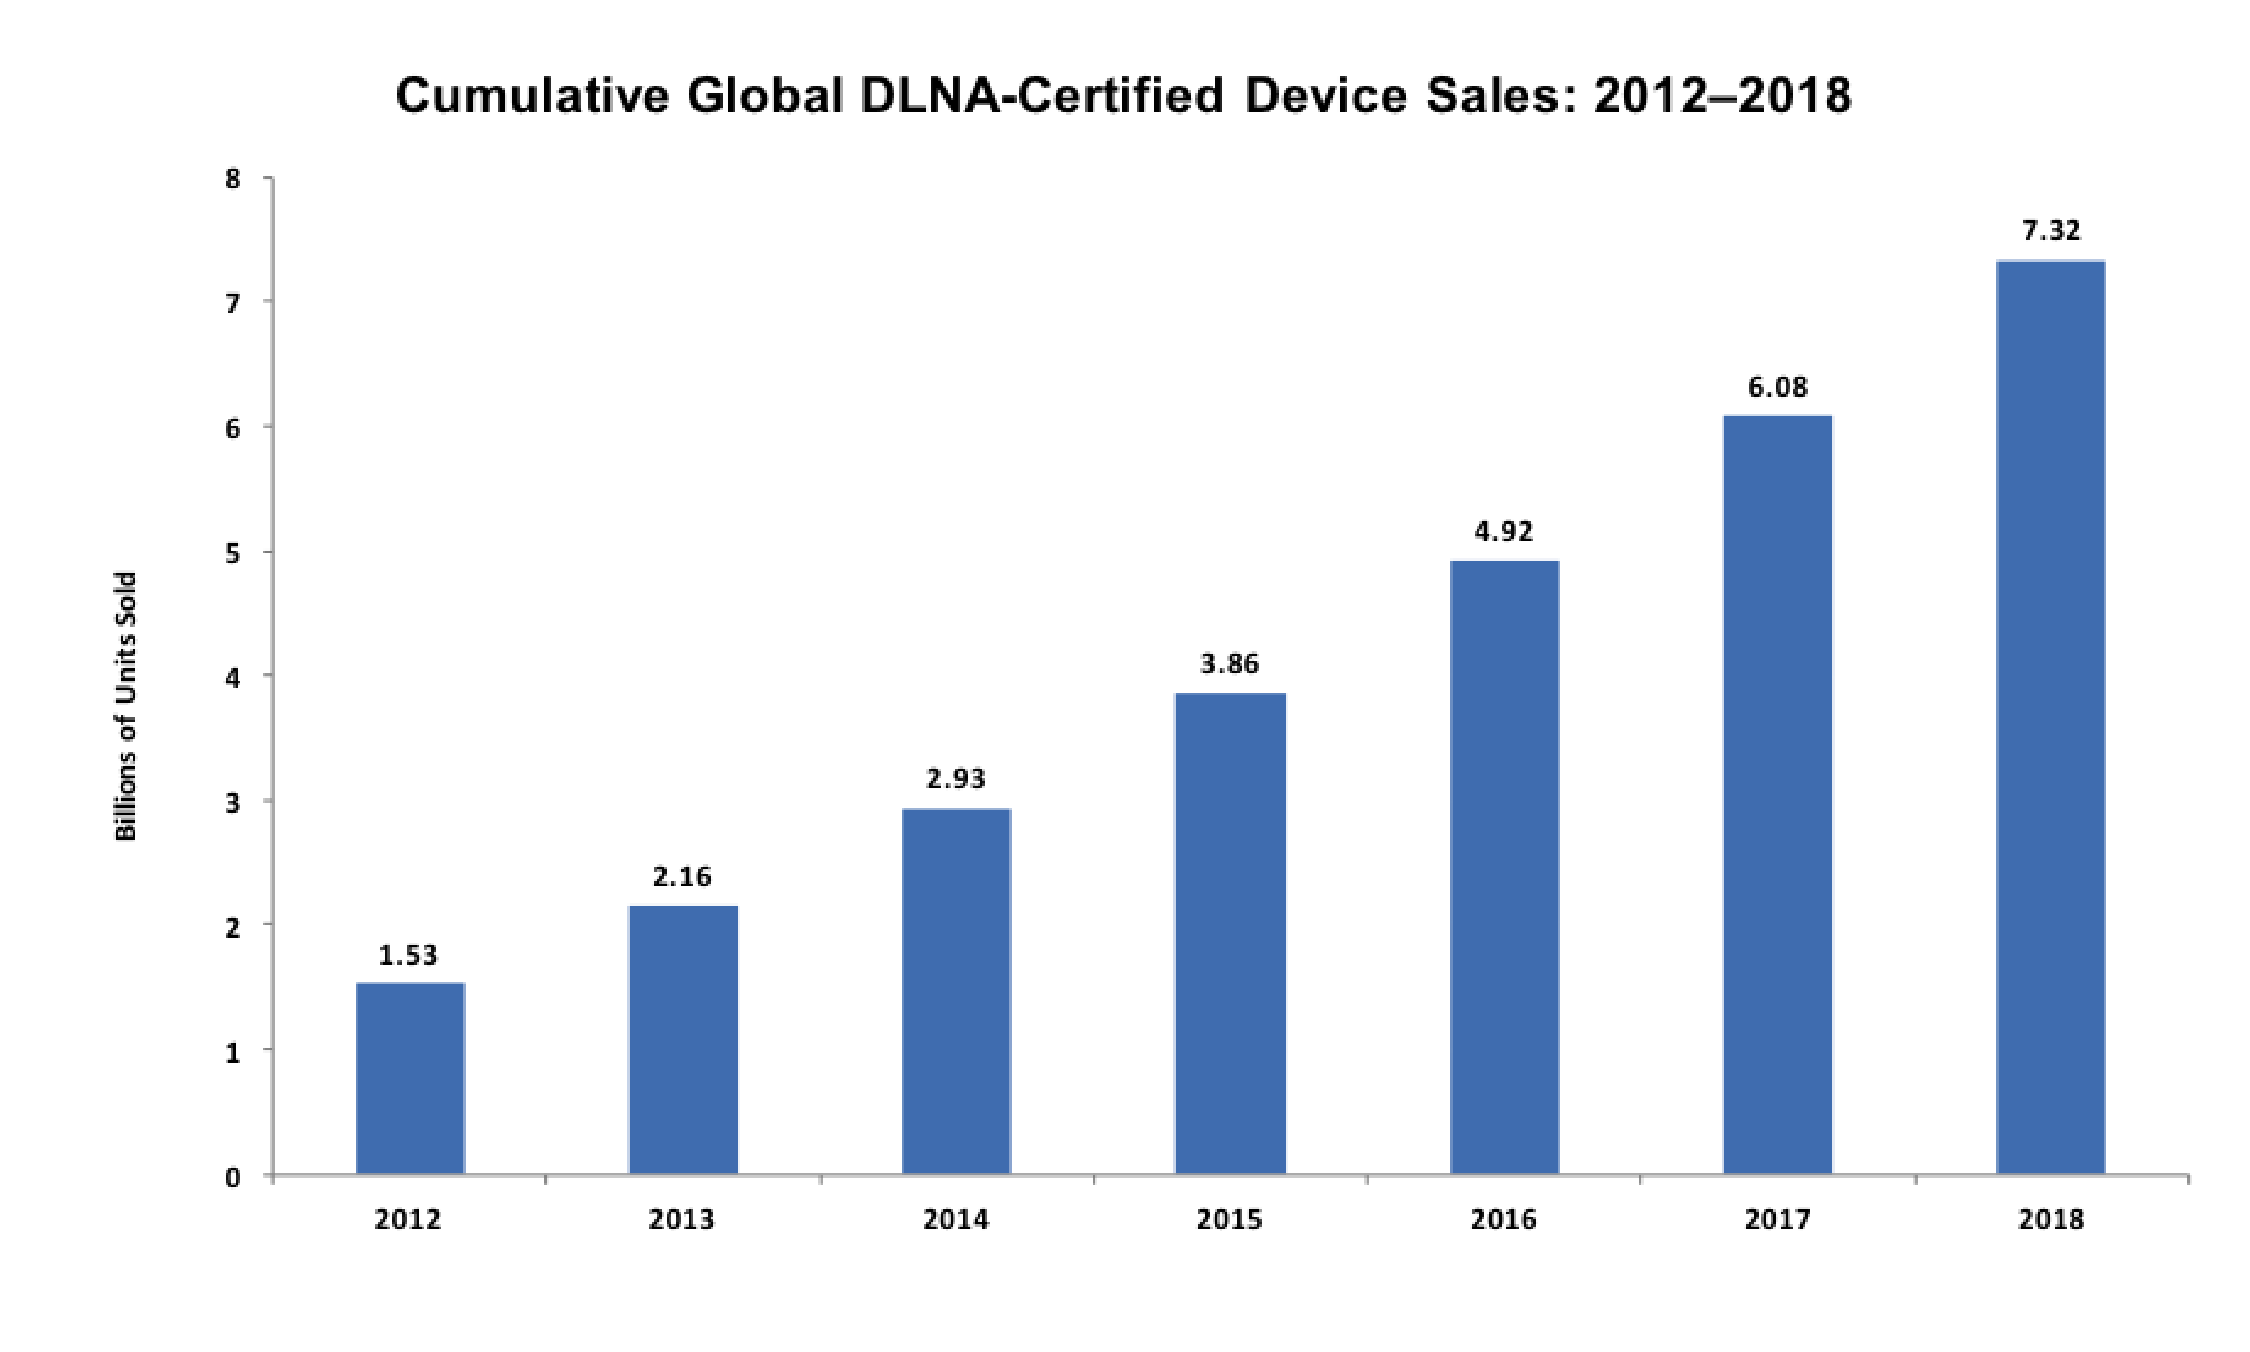
\includegraphics[height=9cm]{charts/dlna_market} 
\caption{Cumulative Global DLNA-Certified Device sales \label{dlna_market}} 
\end{figure} 

\item[--]AirPlay is bundled with Apple products. With great sales of Apple TV, Airport Express, 
Mac, iPhone, iPad, iPod, many families have become accustomed to use Apple's product for everything. In this sense AirPlay has become the easiest way to build home networking solutions. Moreover, it could be the only solution for Apple users, since a lot of speaker manufactures implement their own AirPlay receiver on their AirPlay compatible speakers. And indeed AirPlay provides enough easy to use features for daily usage. 
\item[--]Bundled with Android operating system, Miracast has experienced a fast growth in 
the past two years. Many TVs have been built with Miracast support, to accept peer-to-peer Wi-Fi direct connection. 
\item[--]Chromecast dongle is a cheap device that everyone wants to try. It can be used to easily upgrade an old TV to a "Smart TV".  What's more, since Google has provided good content support for Chromecast dongle, it has soon been accepted by huge amount of users. 
\end{itemize} 

\subsubsection{Technology feature} 
\begin{enumerate} 
\item Media format support \\ 
AirPlay and Chromecast has very limited media format support, since there are 
only limited Apple device types. For example, Chromecast has only released 2 devices so far and there is not much change in the media format. Similarly Apple TV, even in its third generation,  has merely seen the improvements in its high definition supports, rather than the changes in media format support.  \\
\\
In contrast, DLNA not only specified mandatory media formats such as LPCM, JPEG  and MP4, but provided a lot more optional media formats in its specifications as well. \\
\\
Since Miracast is a screen mirroring technology, all formats that can be played on a device are supported in Miracast streaming. Consequently, there is no mandate on media format in Miracast.  

\item Networking technologies used \\ 

A short technology specification comparison is made to help better understand
the existing solutions. Table \ref{Table1} below shows the main technology used 
in different popular solutions. 
%% table 1, compare technology 
\begin{table}[htb] 
\caption{Technology used comparison\label{Table1}} 
\begin{center} 
\fbox{ 
\begin{tabular}{c|l|l|l}  
\textbf{ } & Device discovery & Control Protocol & Streaming protocol \\ \hline 
\textbf{DLNA} & SSDP & UPnP & HTTP \\ \hline 
\textbf{AirPlay} & Multicast DNS & HTTP & HTTP/RTSP \\ \hline 
\textbf{DIAL} & SSDP & Chromecast & HTTP \\ \hline 
\textbf{Miracast} & Wi-Fi direct &  & Wi-Fi direct 
\end{tabular} 
} 
\end{center} 
\end{table} 

Compared to some standards which only provide basic features, others also offer advanced 
features, including screen mirroring. Table \ref{Table2} below shows 
the advanced features provided by different solutions
%% table 2, compare advance feature 
\begin{table}[htb] 
\caption{Advanced feature comparison \label{Table2}} 
\begin{center} 
\fbox{ 
\begin{tabular}{c|l|l|l|l}  
\textbf{ } & DLNA & AirPlay & Chromecast & Miracast \\ \hline 
\textbf{Screen mirroring} & No & Yes & No & Yes \\ \hline 
\textbf{Multiple connection} & Yes & No & No & No \\ \hline 
\textbf{Authentication} & No & Yes & No & Yes 
\end{tabular} 
} 
\end{center} 
\end{table} 


\end{enumerate} 

According to the comparison, each standard has its own features and uses 
different protocols to communicate. There are, however, many common features and protocols that are supported by most standards. For example, the HTTP protocol is frequently used to handle video 
and photo streaming, by many streaming solutions. Another example is that the UPnP device discovery protocol SSDP is commonly used for device discovery. \\
\\
Since multiple standards share the commonly used protocols in their implementations, it is possible to make an application that is aware of all these common protocols. In this sense, making such a mobile application to connect multiple types of devices in a home network can be a good solution to home-networking interoperability. 


\clearpage
\vspace*{100px}
\section{Developing a solution for multimedia home networking\label{chapter3}}

%% Developing a solution for multimedia home networking chapter
%% author Liu Peng

To fulfill the need for interoperability among devices in home networking,
Tuxera Inc. started a project named Streambels(later renamed as AllConnect). The
project aims to solve the interoperability issue in multimedia home networking
by making a universal solution that can connect all available devices at home
and allow them to work together regardless of their protocol.\\
\\
Most devices at home are embedded solutions and have their own firmwares; it is
difficult to update or even impossible to upgrade the software running on these
devices. On the other hand, most home network users
 are not knowledgeable enough to 
to manually set up the more advanced
 network features to achieve a certain degree of device interoperability. In addition, most of these network infrastructures are not designed to be easily
 configured. Due to these reasons, building interoperability among different 
 devices through a mobile device seems to be the most straightforward solution. Mobile devices can serve as a quite flexible and programmable portal for
 home networking.  Other advantages of mobile devices include their great
 processing power, networking capabilities, and their wide adoption and
 availability. Through the available platforms and tools, a mobile application
 could possibly be developed to control all multimedia streaming data flows and
 act as a personal access portal for home networking.\\
\\
After a year of development, the team have created an Android
application\footnote{\url{http://allconnectapp.com/}} that can control and connect every known type of multimedia device at home.
Encouragingly, the number of the application users has grown to nearly one
million so far, providing strong proof of the effectiveness of this solution.\\
\\
This chapter proposes the solution we developed for multimedia home networking.
Section \ref{3_1} proposes the solution and introduces the overall architecture
of the proposed solution. Section \ref{3_2} describes the detailed
implementation aspects of our solution. Section \ref{3_3} describes the user
interface and user experience design. Section \ref{3_4} discusses the features
of our solution. Section \ref{3_5} discusses the possibility to extend our
solution to other content sources. Section \ref{3_6} describes the methodology
of software testing and how our solution is tested before releasing to market.
Finally, Section \ref{3_7} introduces the methodology to evaluate our solution.

\subsection{Architecture overview\label{3_1}}
In order to solve the multimedia home networking interoperability problem, the system should be designed to control media playback sessions. Consequently, content navigation, managing receiver device, and media playback should be the most important three components. In the solution, the system architecture consists of three major parts: the device discovery, content management and streaming.\\
\\
The discovery component is responsible for device discovery. As discussed
in \ref{upnp}, UPnP/DLNA devices and DIAL devices utilize Simple Service Discovery
Protocol(SSDP) for device discovery. An application firstly sends an M-Search request over UDP to the IPv4 multicast address 239.255.255.250 and UDP port 1900. Then, the application listens to other devices' responses. A DIAL device will return a response with an Application URL header, while the UPnP/DLNA devices will return a message with an XML body, which provides detailed service URLs and description URLs. Instead of using the SSDP discovery, Apple products, by comparison, use Multicast DNS for device and service discovery. Obviously, in order to support the three types of devices, namely the UPnP/DLNA devices, the DIAL devices and the Apple Airplay devices, we need to integrate these two mentioned discovery mechanisms, namely, the SSDP mechanism and the Multicast DNS mechanism, into our solution.\\
\\
The content management component is responsible for organizing and
 navigating multimedia contents that can be discovered in the home network. In our solution, these content sources include both the local storage of smart phones and DLNA digital media servers that are connected to the home network. As long as the discovered device belongs to the three device types that this solution support, its content could be streamed using the application solution.\\
\\
The streaming component is responsible for streaming multimedia content to the selected multimedia receivers, such as TVs, wireless speakers, set top boxes and so on. In a typical home networking environment, DLNA, AirPlay video/photo, and Chromecast all use HTTP streaming. The only exception, AirPlay music, uses Remote Audio Output Protocol (RAOP). Because of this, two types of media servers were integrated inside the application solution. With the application, the built-in RAOP server would handle the AirPlay music streaming, and the built-in HTTP media server would handle streaming of all other types.

\subsection{Implementation\label{3_2}}
Since the application is built upon the Android platform, we conducted studies on the Android system architecture and the Android Software Development Kit (SDK). Thankfully, the Android SDK provides many useful Application Programming Interfaces (APIs) and grants crucial permissions to access necessary services and hardware features, such as the permission to access the Internet , the permission to access the WiFi device state change, the permission to allow WiFi multicast and  the permission to read phone storage. The programming language used in developing our Android Application is Java. However some CPU-intensive works, such as transcoding, have to be implemented in C and then embedded to the application using the Android Native Development Kit (NDK).\\
\\
Since Apple has not provided its official specification for AirPlay, our implementation for supporting AirPlay is mostly written under unofficial guidelines. However, Apple has provided its official Multicast DNS (mDNS) implementation in C. Thus, this piece of code is reused and compiled as a shared native library. Similar with the Airplay support, the support for Remote Audio Output Protocol (RAOP) is
 also implemented under unofficial guidelines. To be specific, the RAOP supporting component includes a UDP server and a TCP control channel.\\
\\
With Tuxera being a member of DLNA , we are able to access the detailed specifications and test tools for DLNA. Moreover,  there are a lot of open source UPnP/DLNA
 libraries available since DLNA is now a popular standard. Specifically, in our
 implementation, we uses a library called "cling"\cite{cling}
 \footnote{\url{http://4thline.org/projects/cling/}}, which provides minimal implementation of UPnP device discovery, description information parsing, and basic message handling. By extending "cling"\cite{cling}, we are able to provide media formats compatibility across different devices.\\
\\
Google has officially provided the Chromecast SDK for different mobile platforms, which enables us to  implement the Chromecast integration with ease. In the Streambels project, the Chromecast integration is built upon the Chromecast API.\\
\\
When it comes to media server implementation, according to the DLNA guideline,
certain additional headers need to be implemented in the stream. This
requires the HTTP server to possess the functionality to add DLNA specific
headers. Another requirement is that the "Seek" action needs to be supported on the server side. To support "Seek", byte based seeking operations are enabled in our implementation.\\
\\
For receivers who do not use the DLNA standard, a basic file server with byte range support will be sufficient to do the work.\\
\\
In order to serve media for all the receivers from both online and local storage, a separate media proxy also needs to be implemented.\\
\\
After investigating and comparing multiple server implementations on Android, we
concluded that NanoHTTPD is the ideal choice for our solution, because NanoHTTPD is easy to use,
Apache licensed, very tiny and efficient. Since NanoHTTPD is minimally implemented, it is also easy to be modified and extended. With NanoHTTPD , additional headers can be easily added to make the server implementation compatible with DLNA receivers. Besides, a proxy is also easy to integrate with  NanoHTTPD.\\
\\
Taking all these technical details into consideration, we devised a simplified
architecture for our implementation, which is shown in Figure \ref{chart3}.
\begin{figure}[htb]
\centering 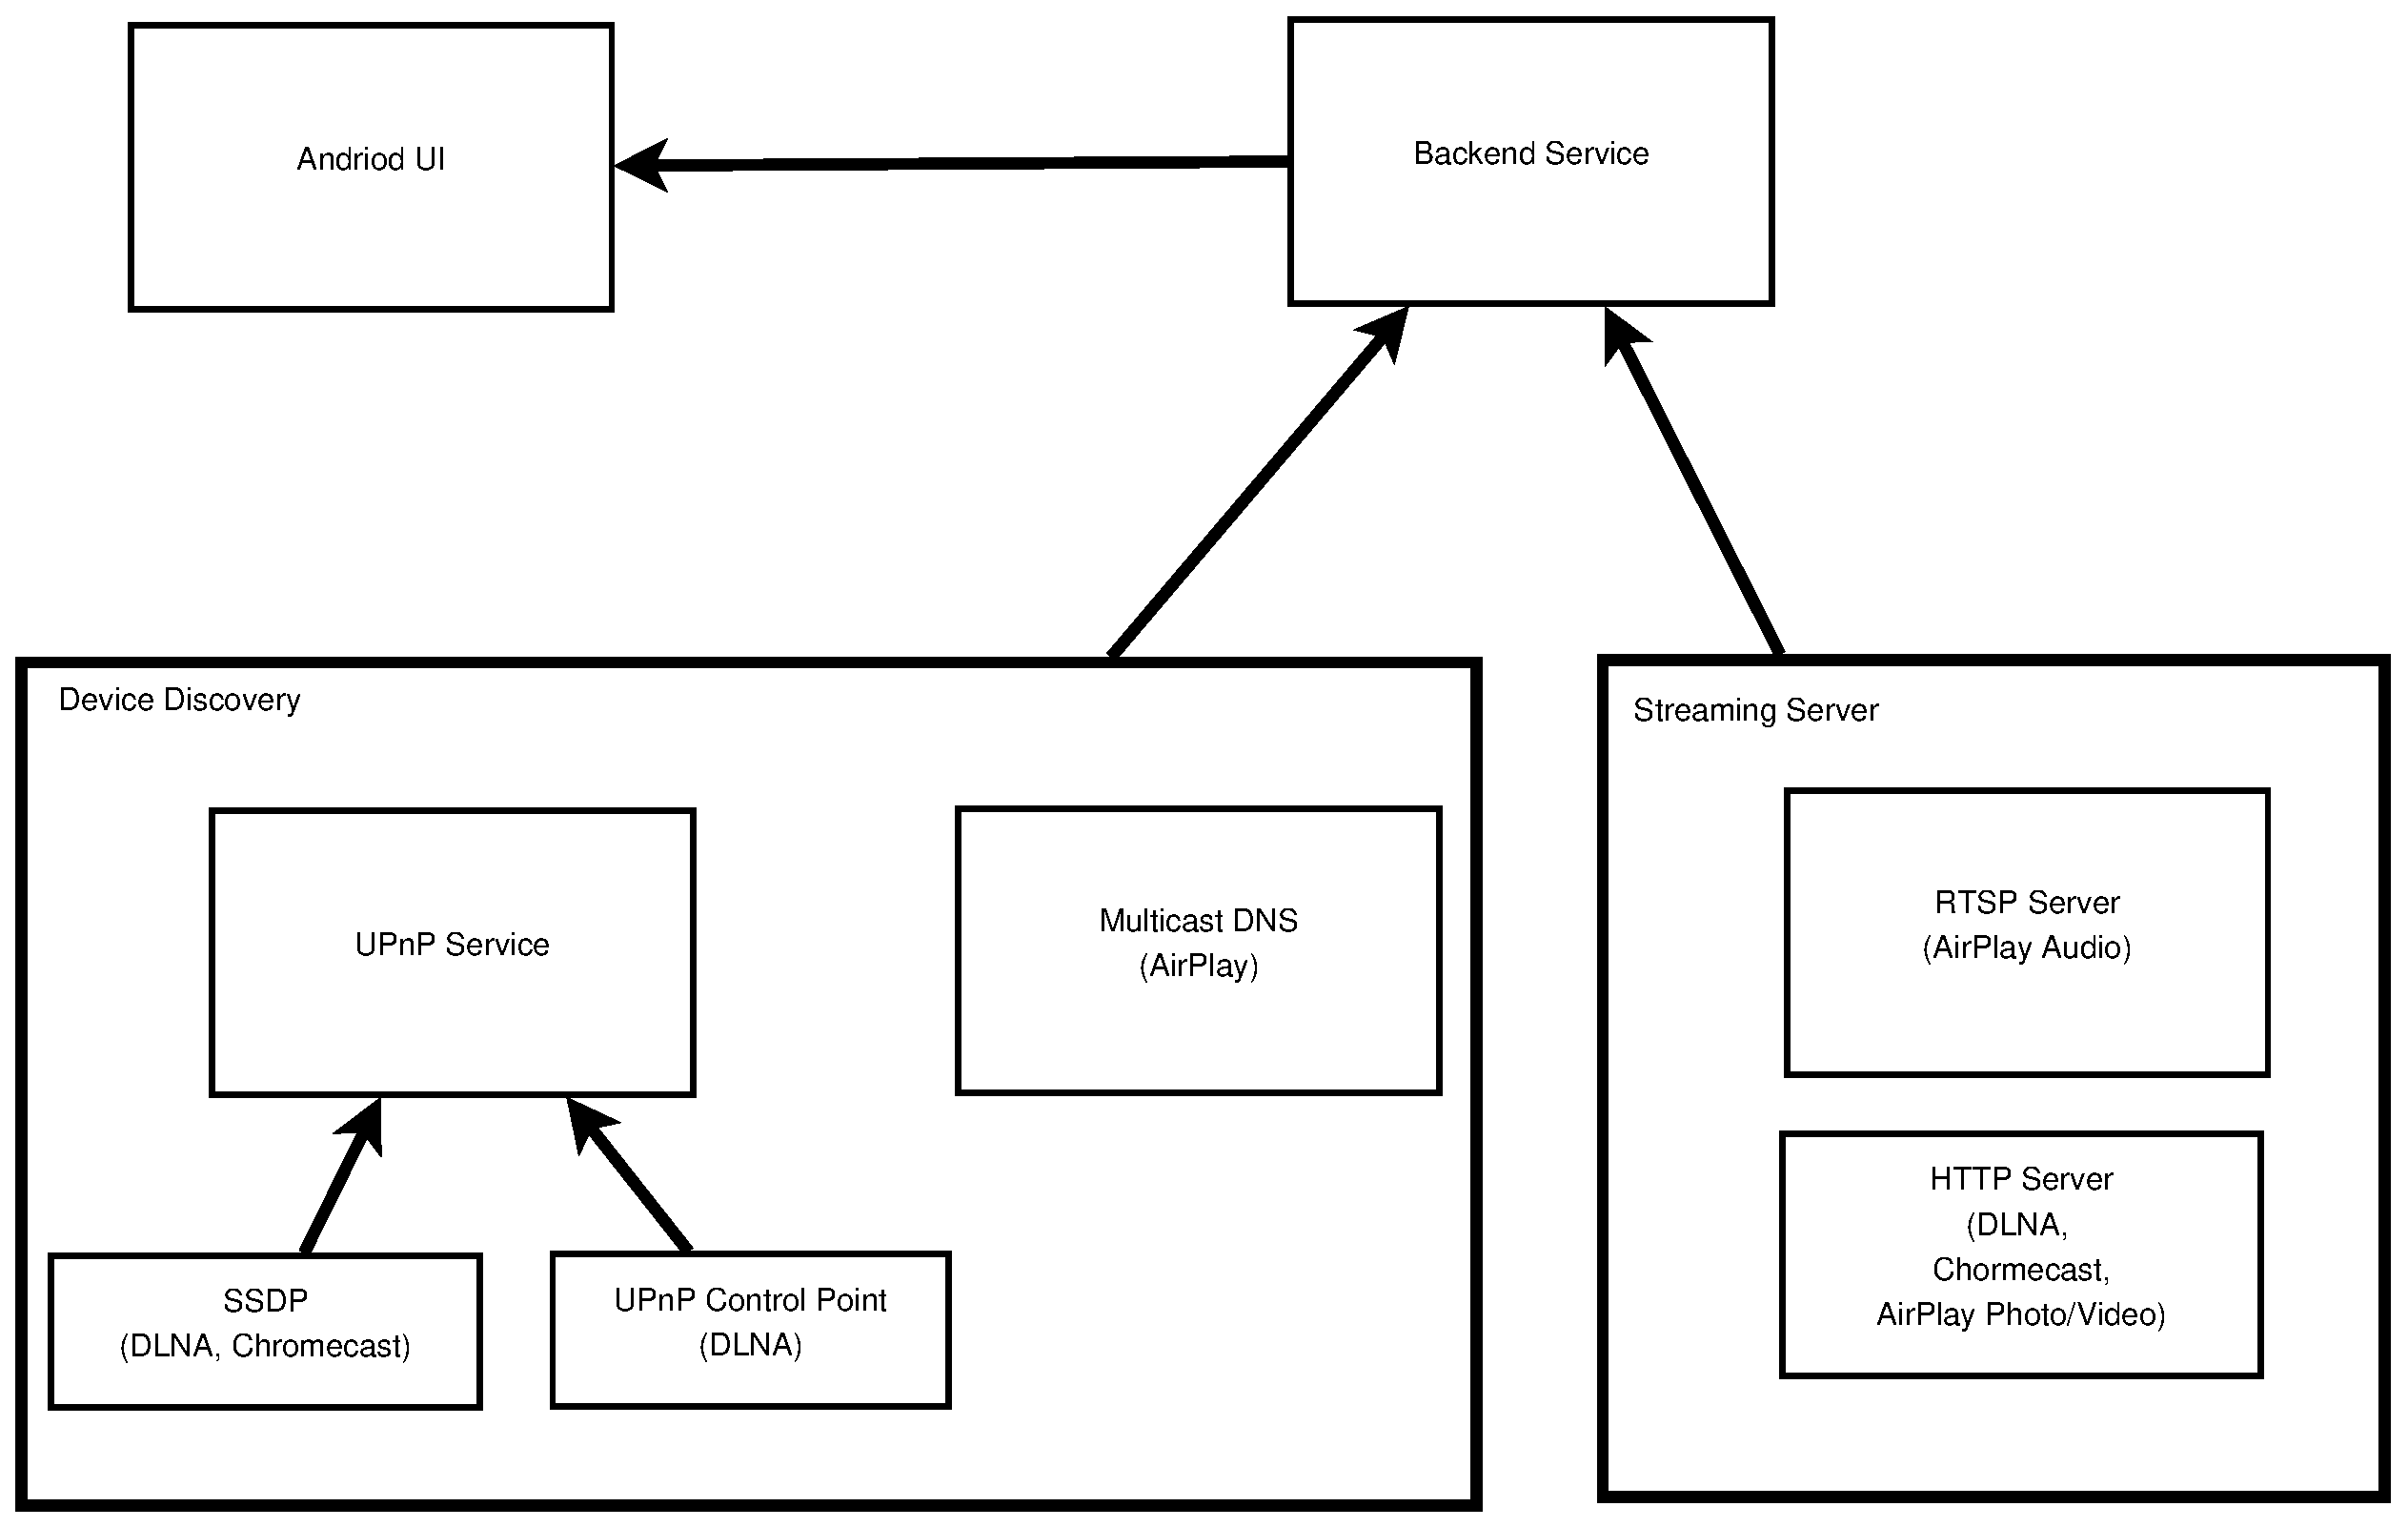
\includegraphics[height=9cm]{charts/chart3}
\caption{Simplified application architecture\label{chart3}}
\end{figure}\\
\\
When streaming content, the data flow is different for different scenarios. Figure \ref{chart4} shows the three use scenarios and their corresponding data flows:\\
\\ 
If the content is stored in a mobile phone, a streaming server in the application will be used to stream the content from phone to the selected receiver.\\
\\
In contrast, if the content is located on the Internet and the receiver is a DLNA Media Renderer, a proxy will be needed. To be specific, the proxy will first download the resource stream and then add certain headers required by the DLNA specification. After that, the proxy streams the modified content to the selected DLNA Media Renderer.\\
\\
Finally, if the streamed content locates in a DLNA Digital Media Server, then the source can be used directly by all receivers. In this case, the streaming proceeds directly from the media server to receivers. Our application, in this scenario, will only be used as a control point and do not really participate in the media transmission.\\
\\
\begin{figure}[htb]
\centering 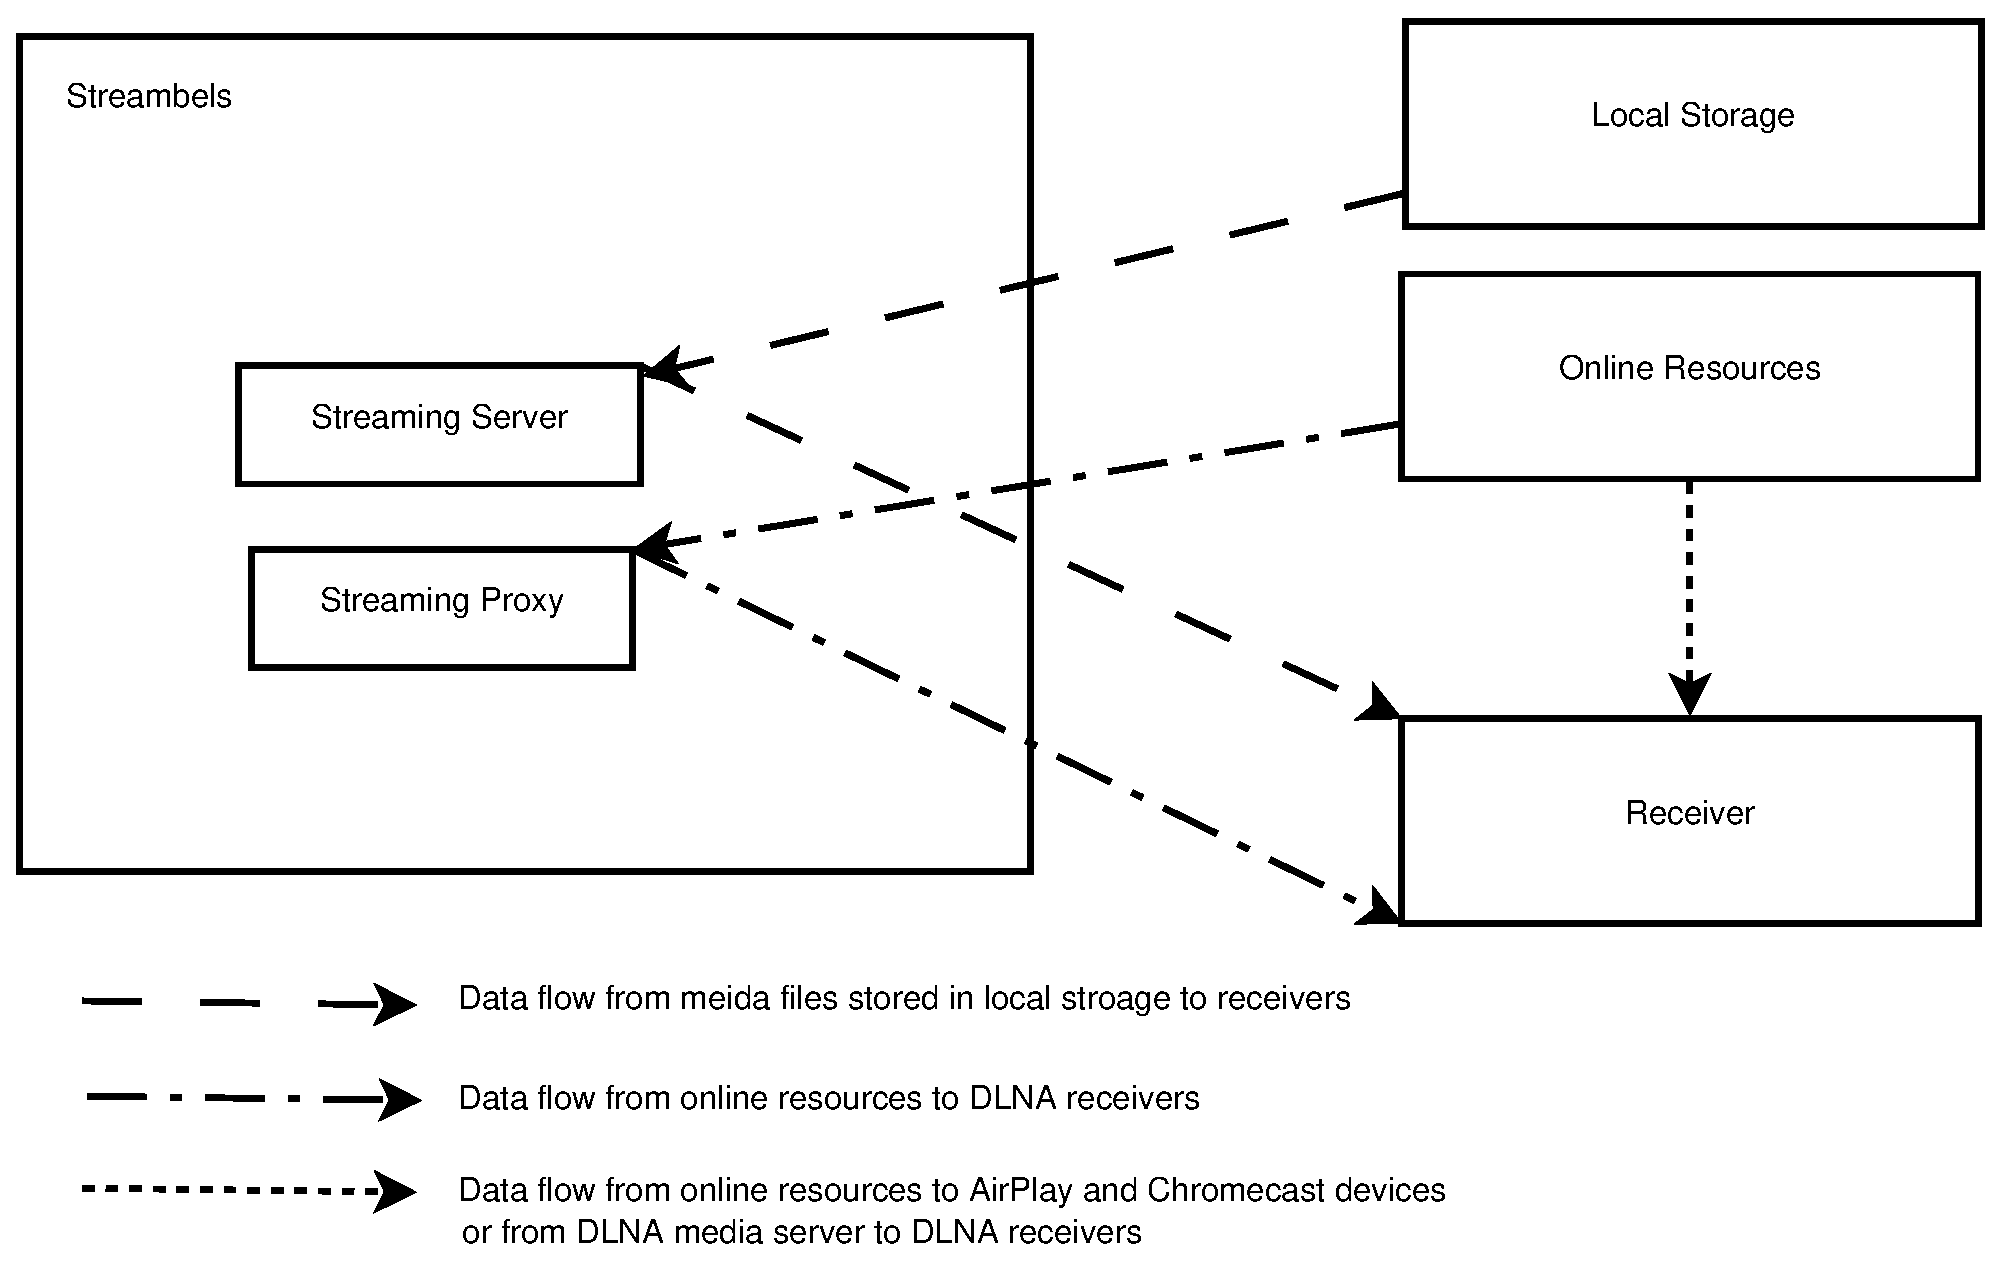
\includegraphics[height=9cm]{charts/data_flow}
\caption{Simplified data flow \label{chart4}}
\end{figure}

\subsection{UX design\label{3_3}}
In terms of UI and UX, the application should be simple enough to use. Users should be able to locate the media, browse
 content on different sources, and follow the data flow between devices without any difficulty. The control of different devices should also be intuitive so that the inter-operation between different devices can be seamless.\\
\\
A multimedia home networking solution should be content centric so that user can easily navigate through different sources. The application is designed similar to a multimedia player. A cast button is added at the top of the application to make it easier to select cast devices. The content is categorized into 4 sections: music, video, photo and online sources. In Android, since the system provides share intent method for inter-activity communication, an interface is also made to manage share intents from other activities, which enables streaming from other on-line content providers. The selected receiver is designed to be visible to user from everywhere inside the application. \\
\\
Bearing all these considerations in mind, the final appearance of the application becomes simple and effective. Figure \ref{chart5} shows the final design of our application.
\begin{figure}[htb]
\centering 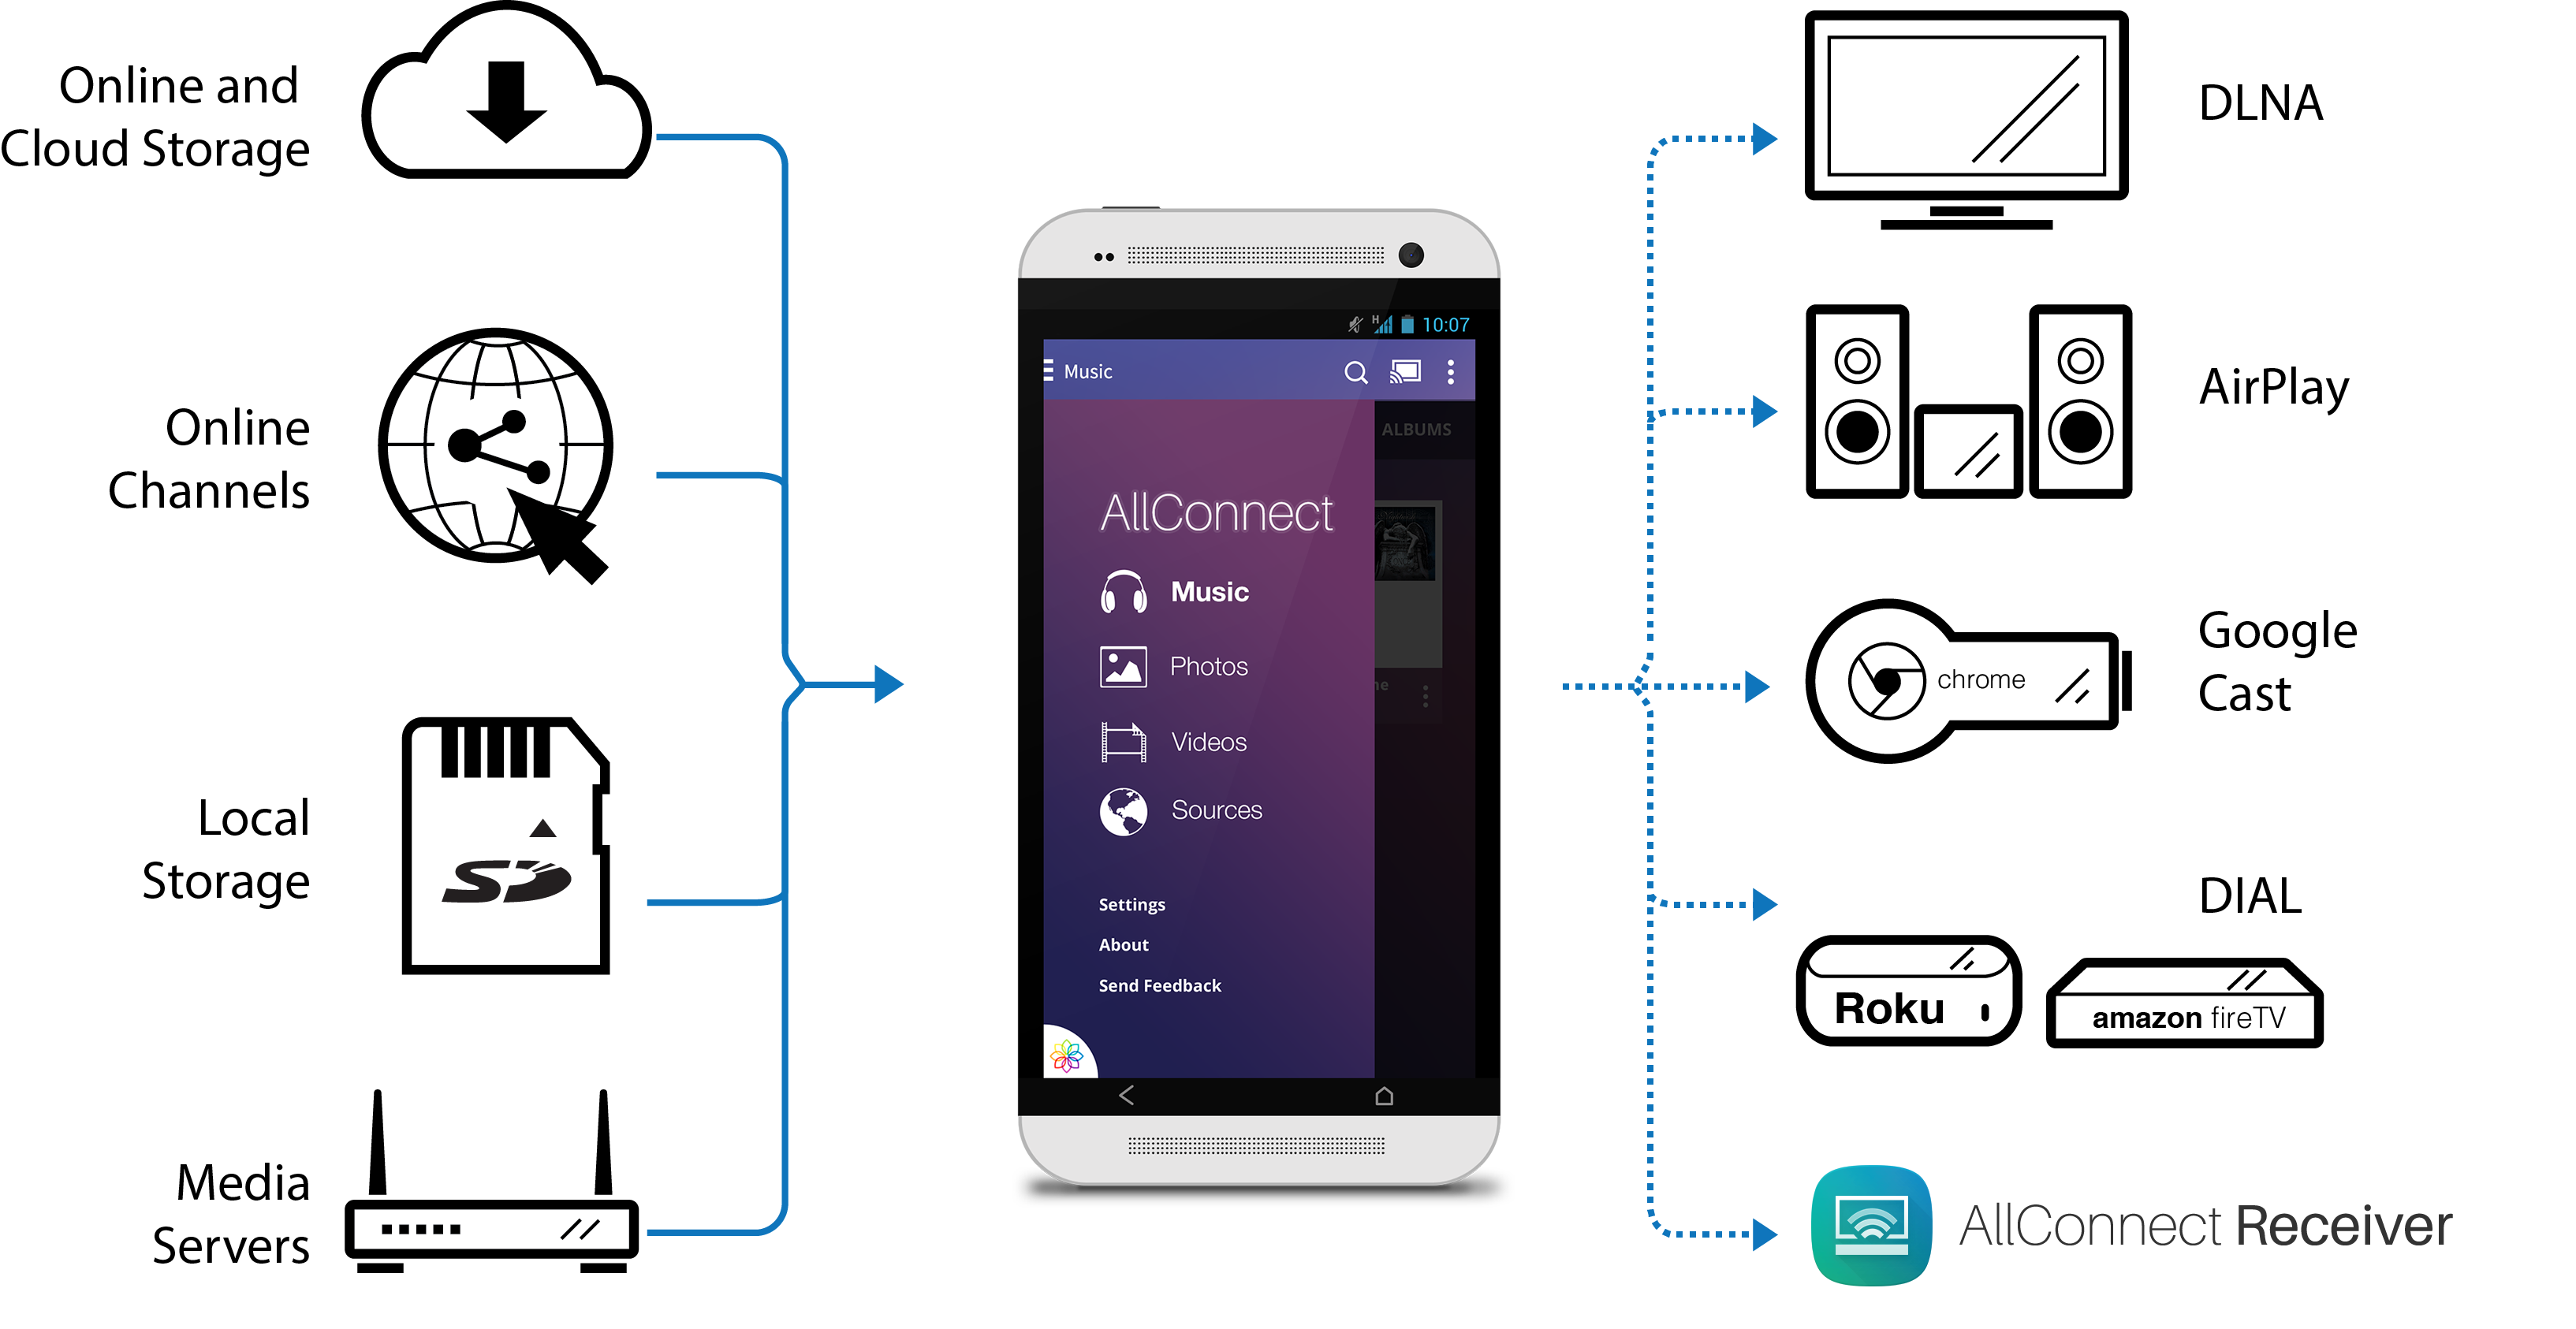
\includegraphics[height=8cm]{charts/allconnect-app}
\caption{Application UX design \label{chart5}}
\end{figure}

\subsection{Features\label{3_4}}
The Android application we have developed can handle most multimedia devices in typical home networking. It also provides various features, making it a powerful and universal solution for multimedia home networking.\\
\\
Firstly, the application itself is a multimedia player. Both the media stored locally on the phone storage and the media located in the DLNA media servers can be browsed and played locally on the phone.\\
\\
Secondly, the application is fully compatible with AirPlay, DLNA, Chromecast and FireTV receiver devices. All devices can be discovered as renderer devices.\\
\\ 
Thirdly and most importantly, the application enables the DLNA media server to work together with all kind of receivers regardless of the protocol used. The app served as a bridge for different multimedia receivers and media sources.\\
\\
Lastly, YouTube and other on-line channels like Vimeo and Facebook are supported as available media sources. These content can be streamed, regardless of the protocol, to all supported receivers that are connected to home network.

\subsection{Extensibility\label{3_5}}
Streambels has embedded a media streaming server for local files and a streaming proxy for bridging the gap between online resources and home networking. By using a built-in proxy, Streambels is able to share on-line resources from the Internet to devices in home networking environment. \\
\\
New service providers and content providers can integrate home networking support into their products easily by just sending formatted intent to our application following our guidelines. The proxy will automatically bridge the gap between the Internet and home network.\\
\\
The proxy system provides great extensibility and makes it possible to connect home networking to Internet or Cloud Services.\\
\\
In the future we could also develop a Software Development Kit (SDK) to grant the availability of our technology, enabling other application builders to directly use our home-networking solutions.
\subsection{Test methodology\label{3_6}}
Software testing is extremely important for a modern IT project. Buggy implementations may kill the product in the very beginning since it can badly undermine user experiences. Through testing we could assure the performance and stability of our product. Thus, before the final releasing to the Google Play store, the application was thoroughly tested.\\
\\
These tests included unit test, integration test and functional test.
Unit tests were conducted while coding the application. When each class was finished, unit tests would be written for each method. We also set up an continuous integration server so that each time we commit anything to the git repository, full set of unit tests would be executed. If there were any failure in the unit tests, developer would be immediately notified. Integration tests were done in such a way that we ensured each function module work together with other modules in the system. Lastly, we listed all the possible use cases in paper and prepare a huge media base which contains all kind of media files. With all these preparations ready, manual tests were conducted before the app is finally released in the market.

\subsection{Evaluation methodology\label{3_7}}
This section discusses the methodology to evaluate our application. Section
\ref{3_7_1} describes the experiments to evaluate the performance of Streambels
app. Section \ref{3_7_2} introduces the methodology we use to collect user
activities and user feedbacks.

\subsubsection{Experimental setup\label{3_7_1}}
The test environment is set up as in Figure \ref{setup}. The XBMC
media receiver is running on MacBook A and Streambels is running on a rooted Android phone. Both A and B are connected to a router C using the 802.11 ac wireless interface. \\
\begin{figure}[htb]
\centering 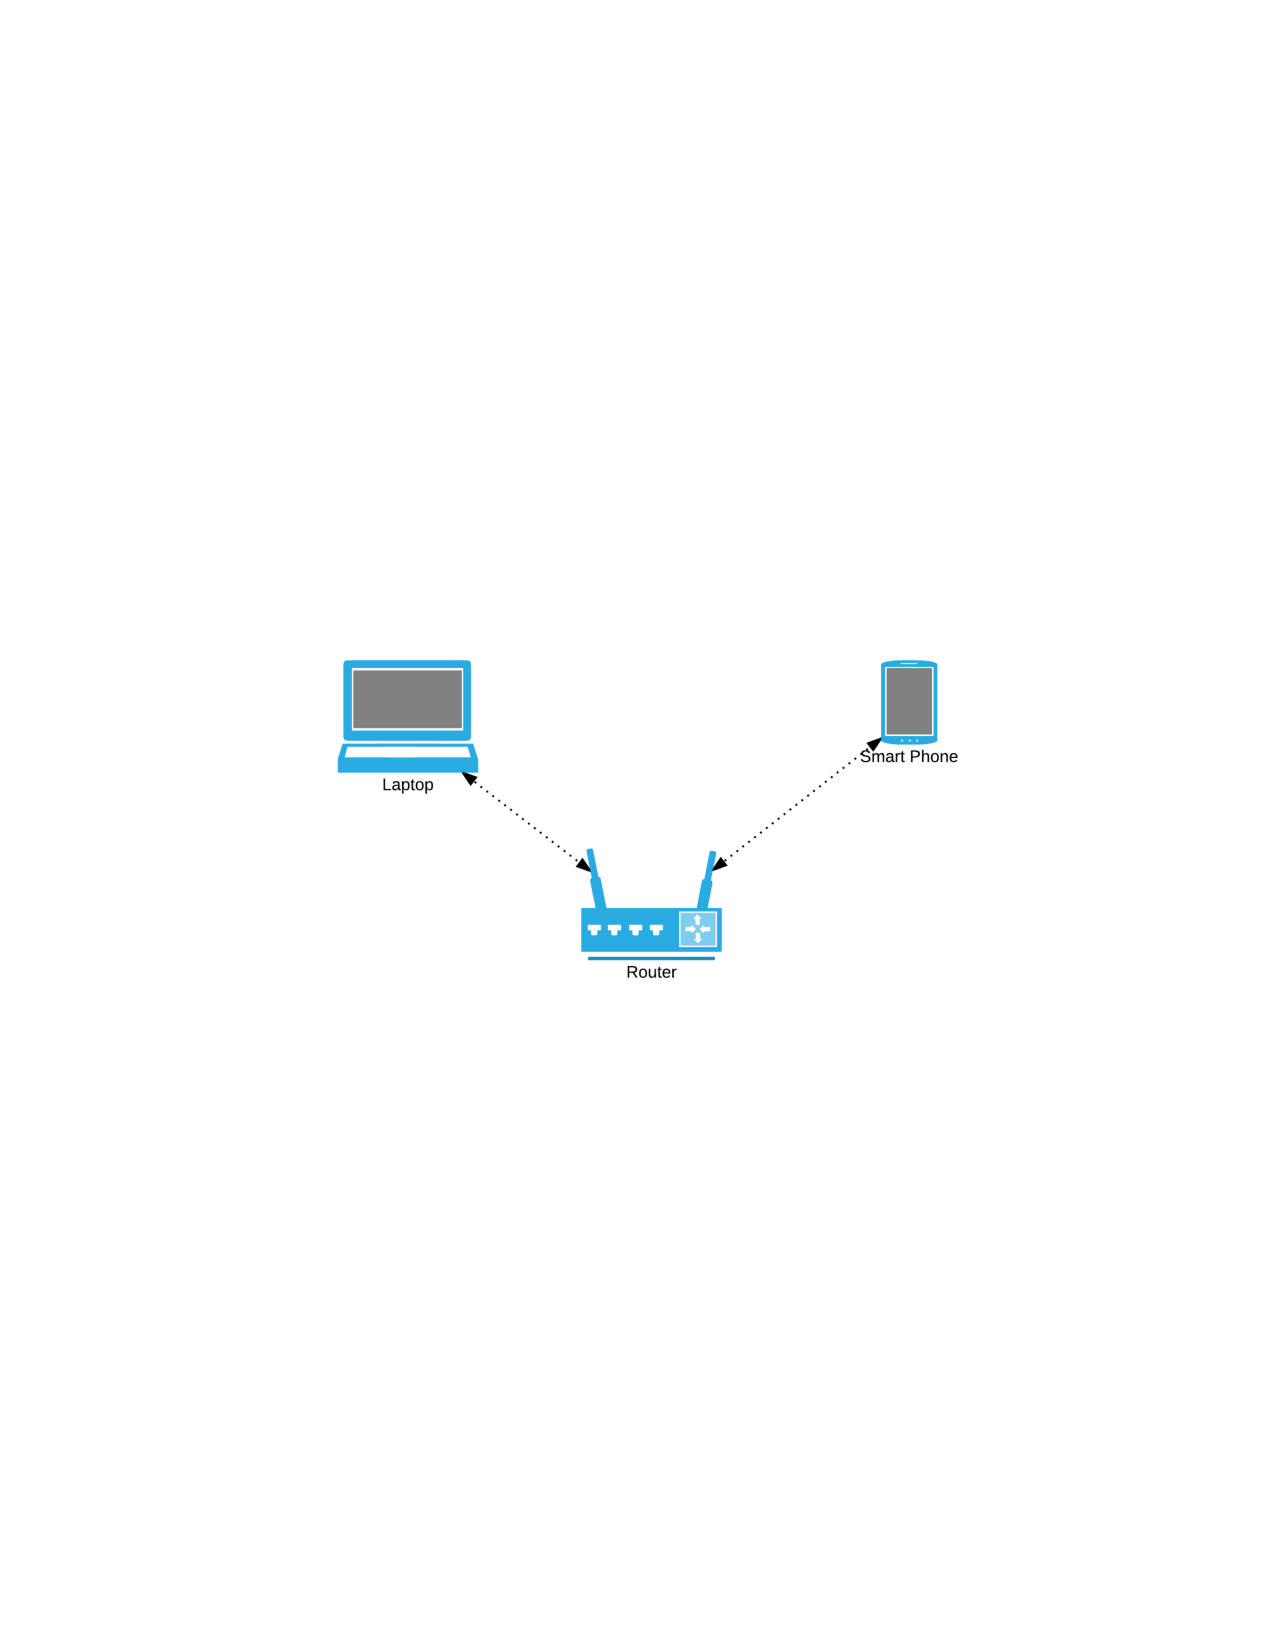
\includegraphics[height=7cm]{charts/experiment_setup}
\caption{Experiment setup \label{setup}}
\end{figure}
With the support of both AirPlay and DLNA protocols, XBMC is an open source media center software that can run on different platforms. It is a popular software solution that is widely used in home networks, which has been ported to different platforms including Raspberry PI.\\
\\
Network Link Conditioner is an application provided by Xcode that runs on Mac to emulate network conditions, such as packet loss, network delay and bandwidth variations. By changing the configurations, different network conditions can be set to determine the boundary network conditions.\\
\\
Wireshark is an useful developer tool to capture and analyze network traffic. It can be installed on both the sender and receiver side. However, it can only be installed on rooted Android phones to gain the access to network interface on Android. In our setup, Wireshark is installed on MacBook because we need to adjust network condition on the receiver side and there might be packet loss since some protocols may use UDP protocol.\\
\\
When the test starts, the same content will be streamed to receivers using two different standards, AirPlay and DLNA. The same test will be run several times to get the average statistics. Different parameters will also be tested by using different network condition configurations.
\\
3 parameters are taken into consideration when conducting the tests: bandwidth, packet loss and delay. 
\subsubsection{User study and feedback collection\label{3_7_2}}
Since the product is targeted to Android market and is directly used by end users, user feedback is really important to us for improving the product continuously. Email is used for normal communication between the user and our support. A submission window is built inside the application, so that users can easily send feedback to us directly by Email.\\
\\
There is no perfect program, crashes sometimes happen. Thanks to Google, all crash reports are collected and displayed inside developer console. This makes it a lot easier to track and debug our application.\\
\\
Inside Streambels, we also integrated Google's Analytics API. The API provided great convenience for us to collect number of users and sessions every day. Other information such as operating system version, application version and the number of active users as well as user feedbacks, have helped us to gain more insight in our application and the market response, making it easier for us to improve the application and do better marketing.\\ 
\\
It is also interesting to see what kind of technologies are most used in their daily life. With the Google analytics SDK, we could trigger events when user select their receivers. After months of monitoring and statistics collection, we have been able to figure out the most popular standards and most popular online channels .\\
\\
These valuable information will in turn help our decision making on how we should improve our application. Some of these result will be discussed in Chapter \ref{chapter4}.

\clearpage
\vspace*{100px}
\section{Results\label{chapter4}}

%% Resluts chapter
%% author Liu Peng

After designing, implementing and testing the software. We started several
evaluation tests on the streaming performance, and we have released the
application to public in Nov 2013. So far, we have improved the application a
lot and also brought many new features to it. As discussed in previous chapter,
we used Google Analytics SDK to help us get insights to our application and our
users. In this chapter we will present and analyze those results.

\subsection{Performance}
In terms of streaming, our solution include two major streaming components. It
would be helpful to study how the media streaming protocol have the better 
performance while streaming multimedia contents. And also, by comparing
different streaming types of media, we could investigate which protocol is best
suitable for certain type of media. Two major streaming technology we
used in our solution are HTTP streaming and RTSP streaming.

Hypertext Transfer Protocol (HTTP) refers to the protocol used to deliver web
pages and images across the Internet worldwide. HTTP is an adopted, open
standard-the most ubiquitous mode of delivery on-line. HTTP is a "stateless"
protocol; think of it as an airline ticket to anywhere. HTTP can be delivered
by a variety of web servers, both commercial and open source.

Real Time Streaming Protocol (RTSP) is a network control protocol used in
entertainment and communications systems to control streaming media servers.
RTSP is used to establish and control media sessions between two points,
usually server and player client. Clients of media servers issue VCR-like
commands, such as PLAY and PAUSE, to facilitate real-time control of playback
of media files from the server. Microsoft's Smooth Streaming is a hybrid
delivery method that acts like traditional RTSP streaming but is based on HTTP
PDL. Apple's HTTP Live Streaming (HLS) is another example of using HTTP to
deliver video with new techniques.

AirPlay uses RTSP streaming for the iTunes music. Thus we chose a mp3 music and
try to stream it to an AirPlay Speaker and an DLNA Speaker, and we used
Wireshark running on rooted Android phone to capture the packets in the network.
The result is presented below, the initial packet count is relatively high,
this is because there is a lot multicast messages in the network for device
discovery, after that, streaming graph shows that after an initial increase in
the traffic, network traffic is relatively stable, this is because the TCP
protocol reaches the best optimized transmission speed.

Next step, we added packet loss in the network, and see the influence to the two
streaming process, result is shown below:
\begin{figure}[H]
\begin{minipage}[b]{0.45\linewidth}
\centering
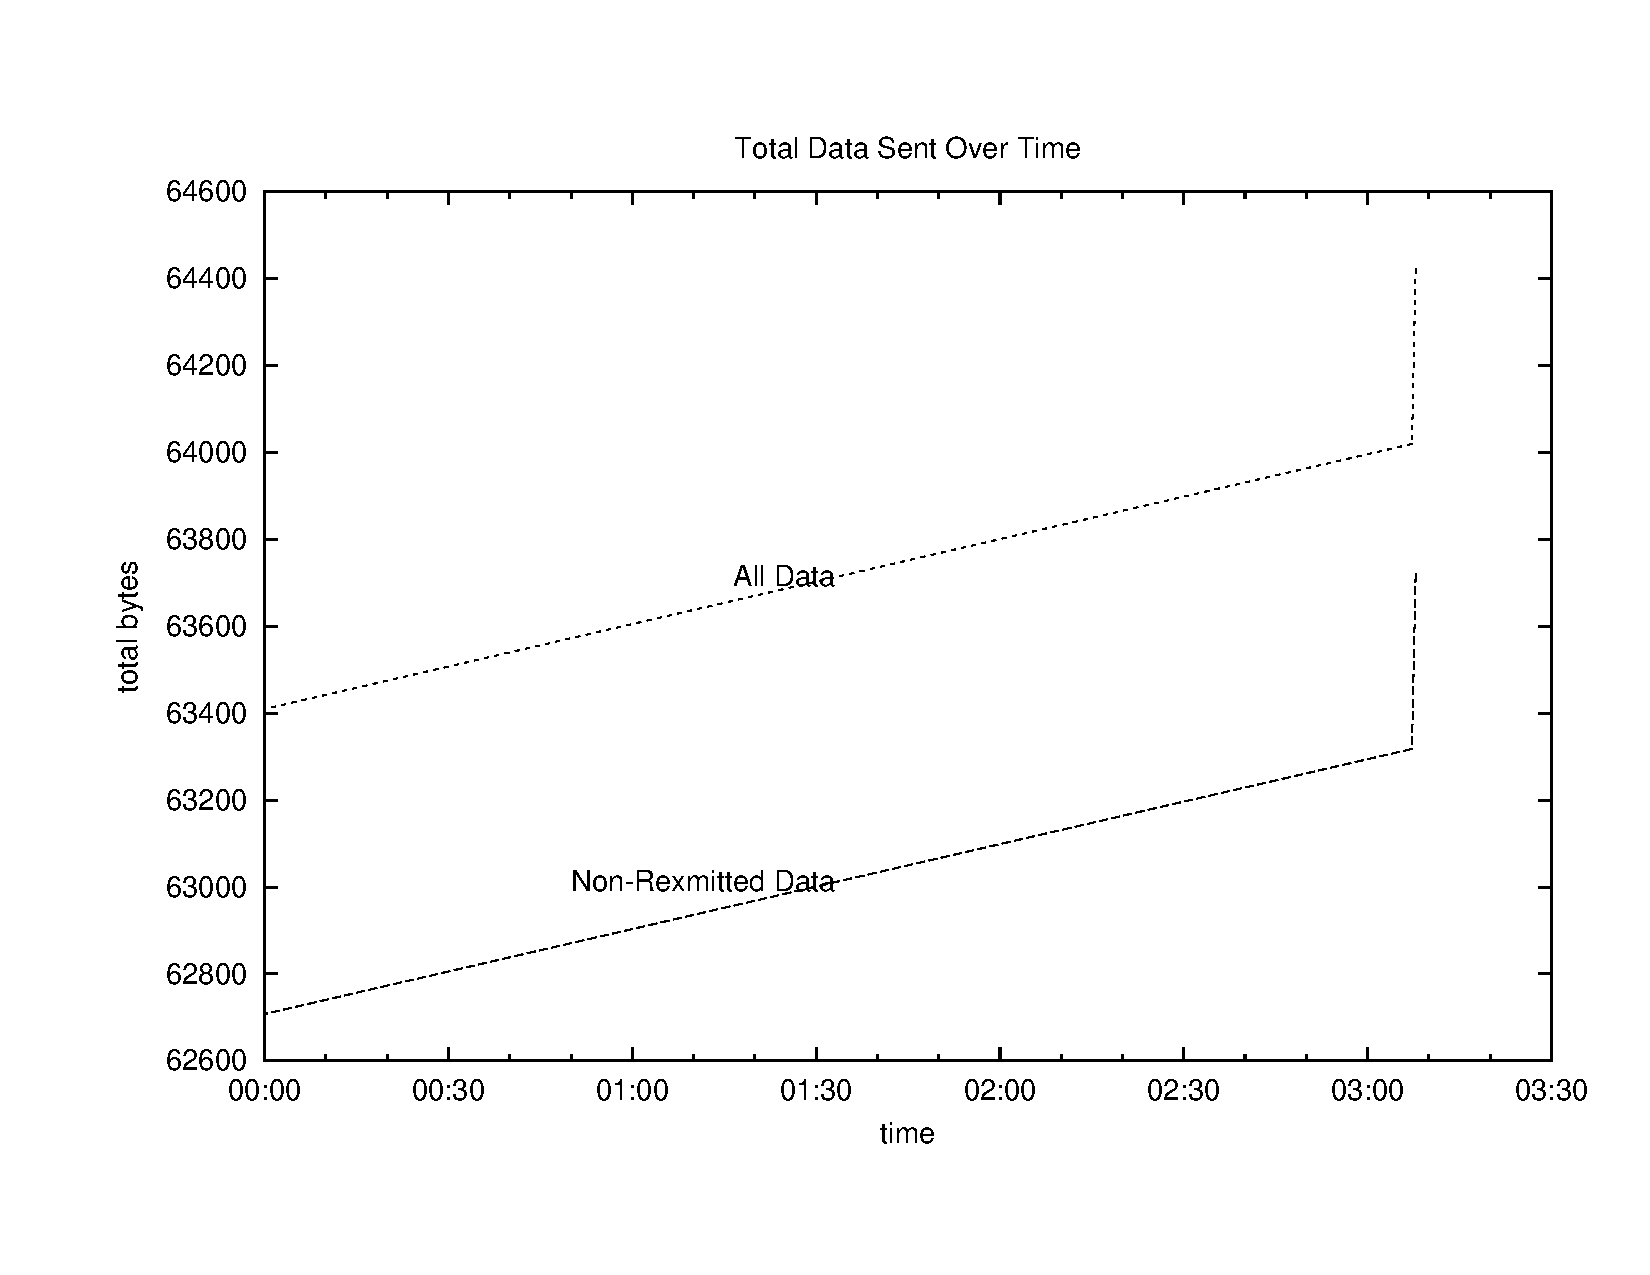
\includegraphics[width=\textwidth]{charts/airplay_traffic_data}
%%\hspace{0.1cm}
\end{minipage}
\begin{minipage}[b]{0.45\linewidth}
\centering
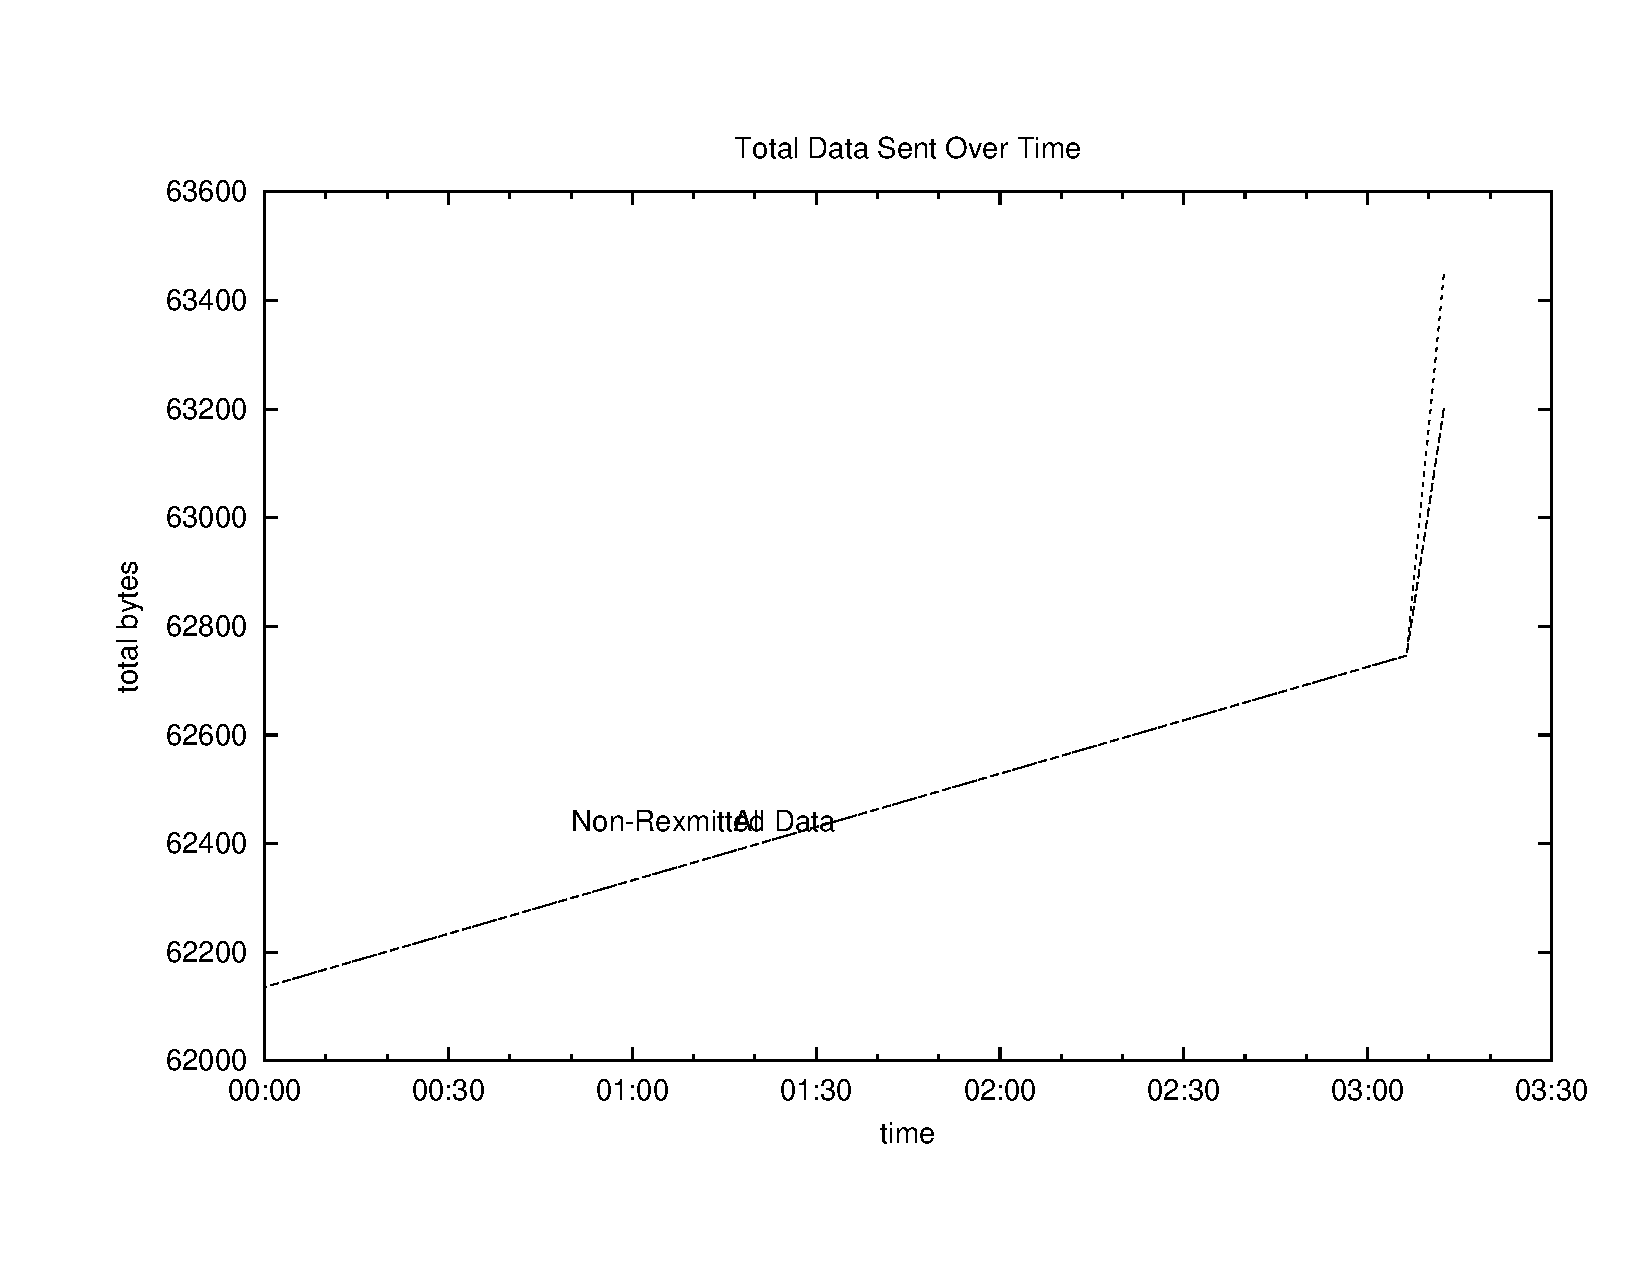
\includegraphics[width=\textwidth]{charts/airplay_traffic_5loss_data}
\end{minipage}
\begin{minipage}[b]{0.45\linewidth}
\centering
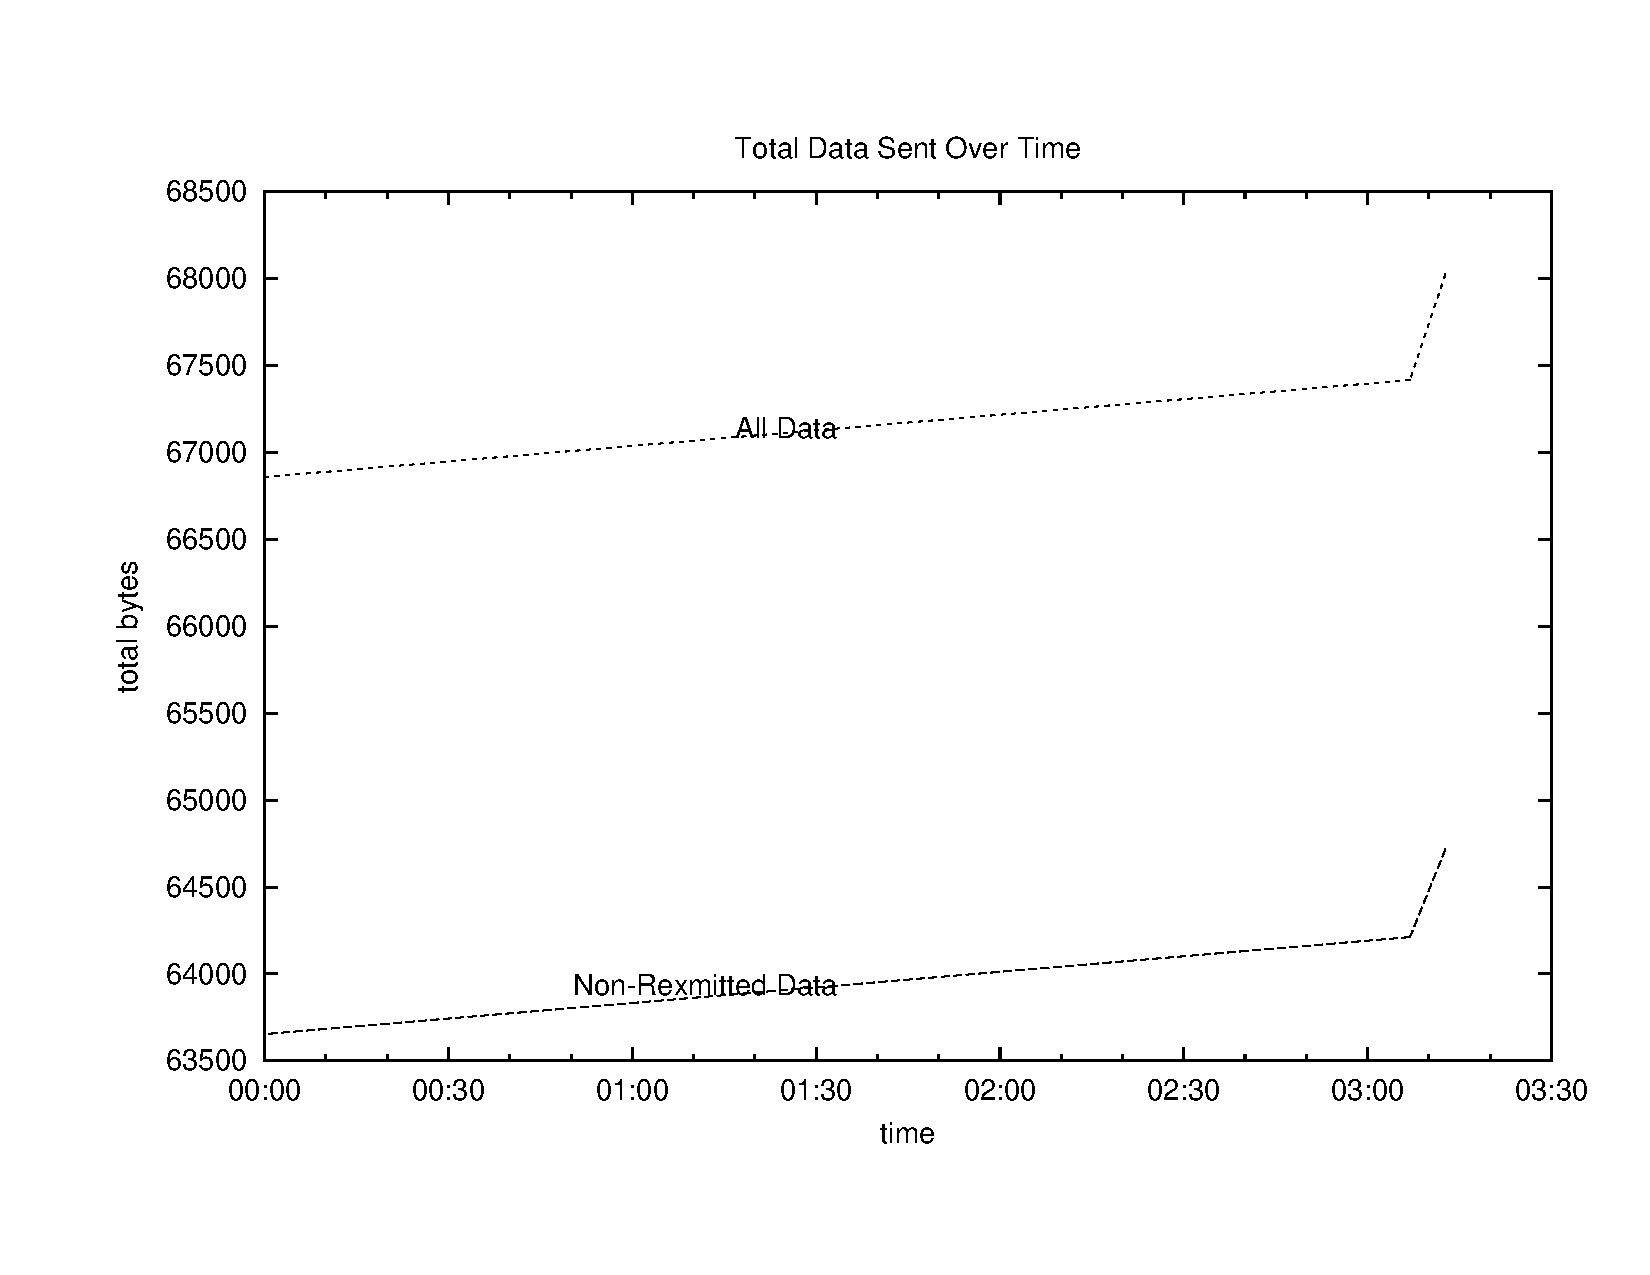
\includegraphics[width=\textwidth]{charts/airplay_traffic_10loss_data}
%%\hspace{0.1cm}
\end{minipage}
\begin{minipage}[b]{0.45\linewidth}
\centering
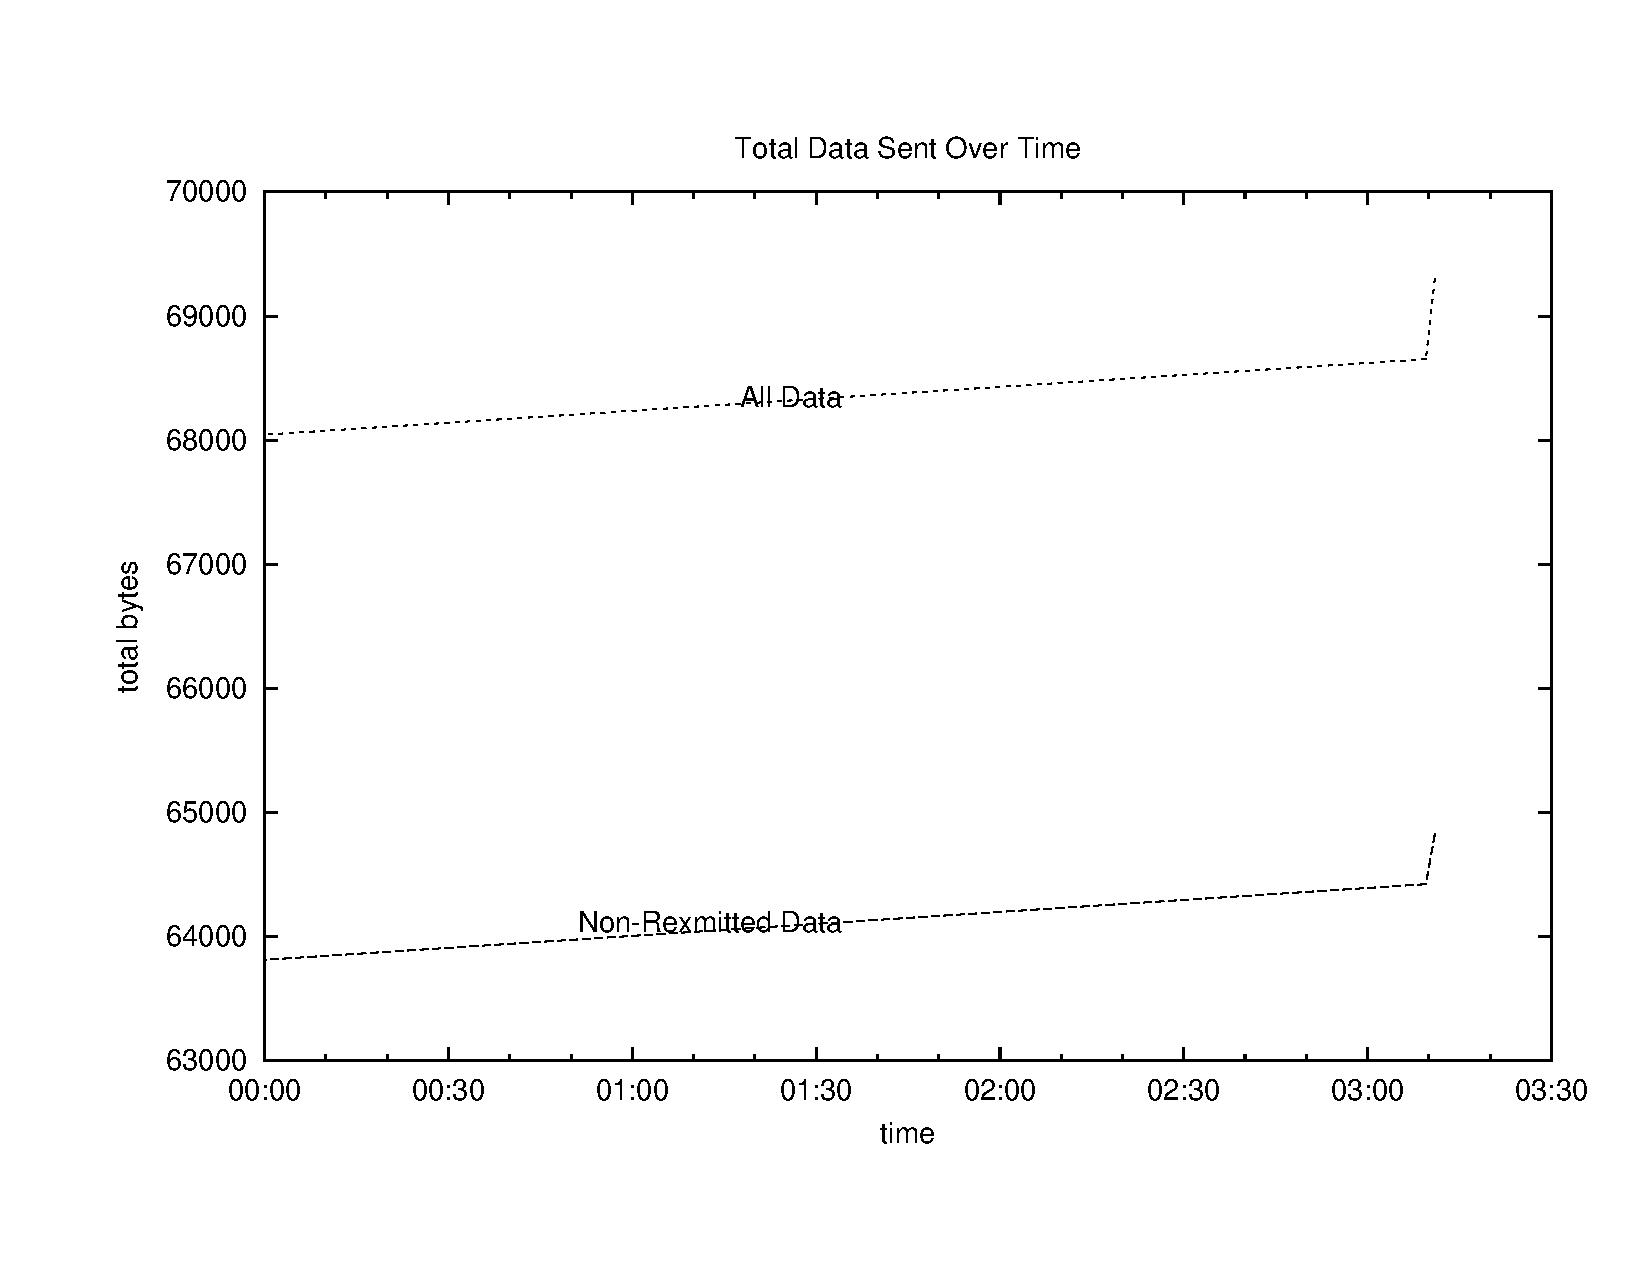
\includegraphics[width=\textwidth]{charts/airplay_traffic_15loss_data}
\end{minipage}
\caption{AirPlay streaming performance in terms of packet loss}\label{multiavp}
\end{figure}



\begin{figure}[H]
\begin{minipage}[b]{0.45\linewidth}
\centering
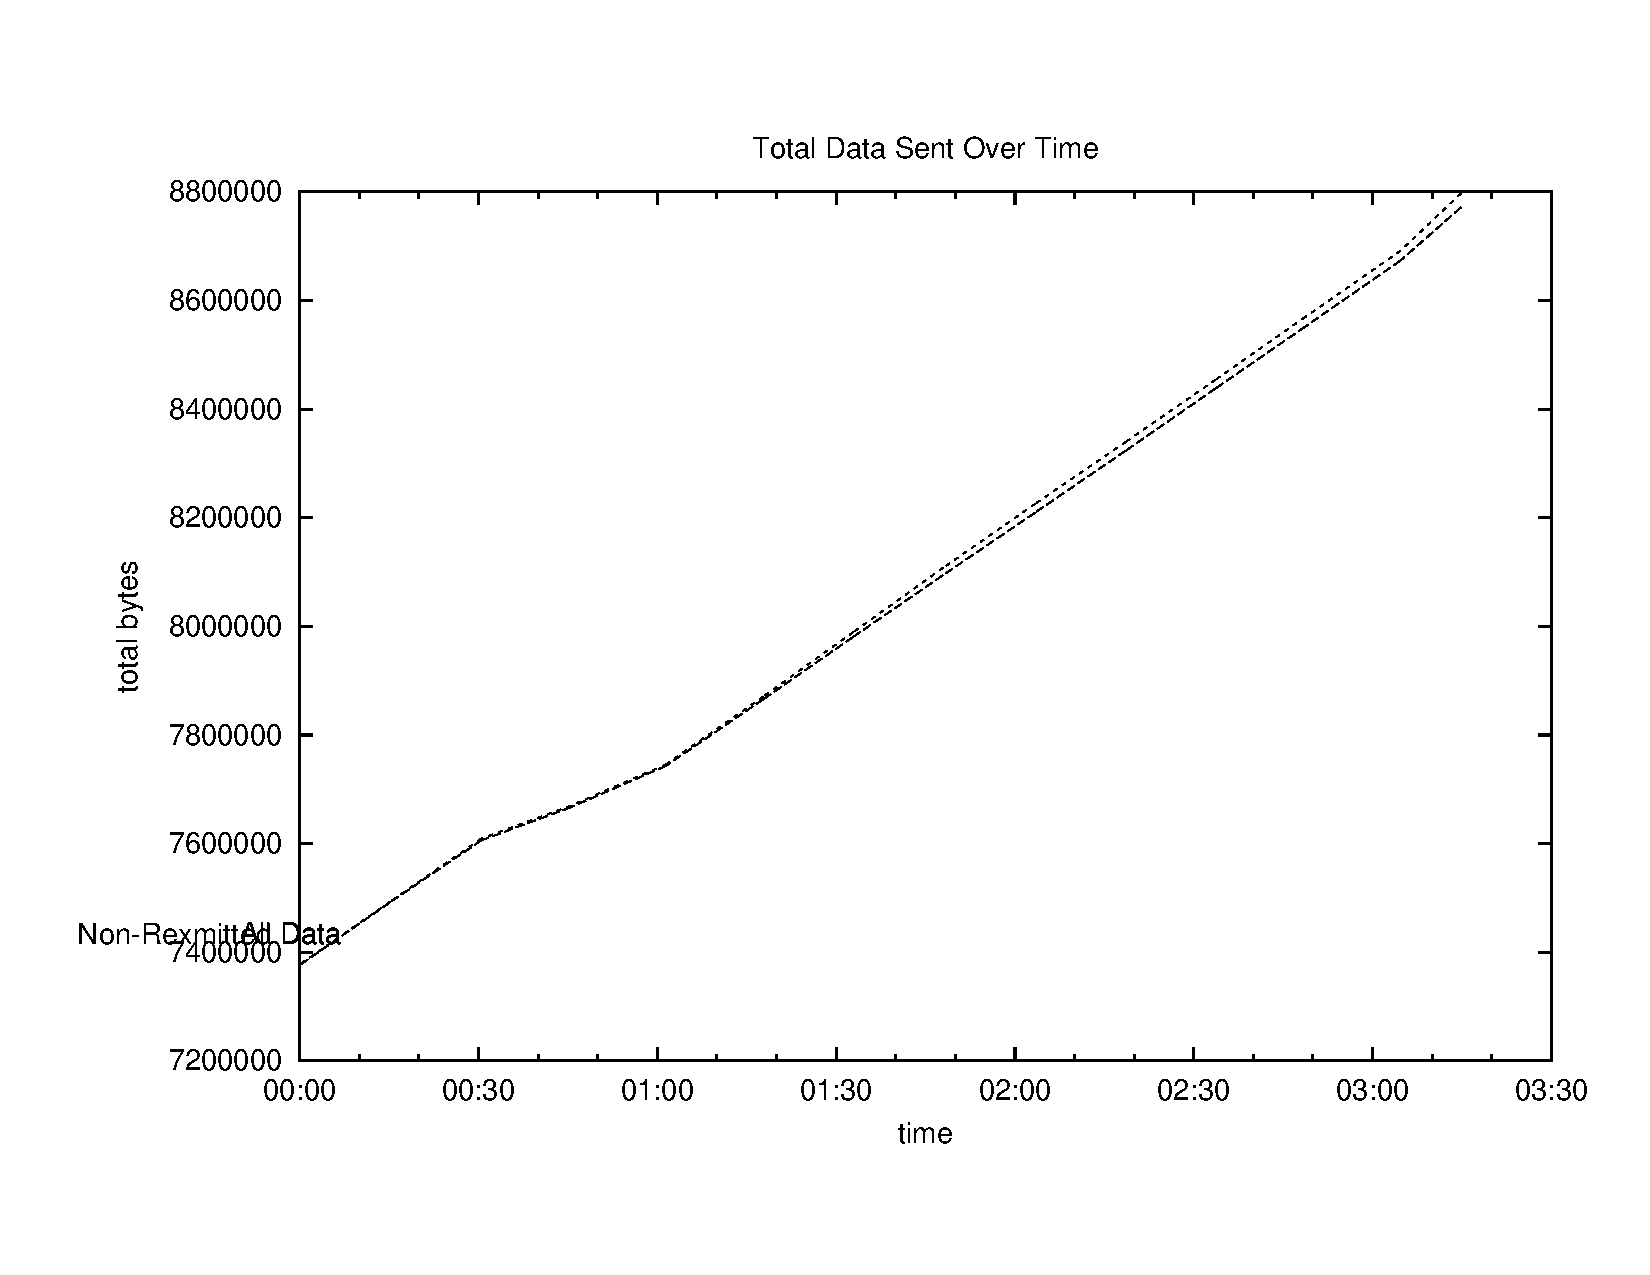
\includegraphics[width=\textwidth]{charts/dlna_traffic_data}
%%\hspace{0.1cm}
\end{minipage}
\begin{minipage}[b]{0.45\linewidth}
\centering
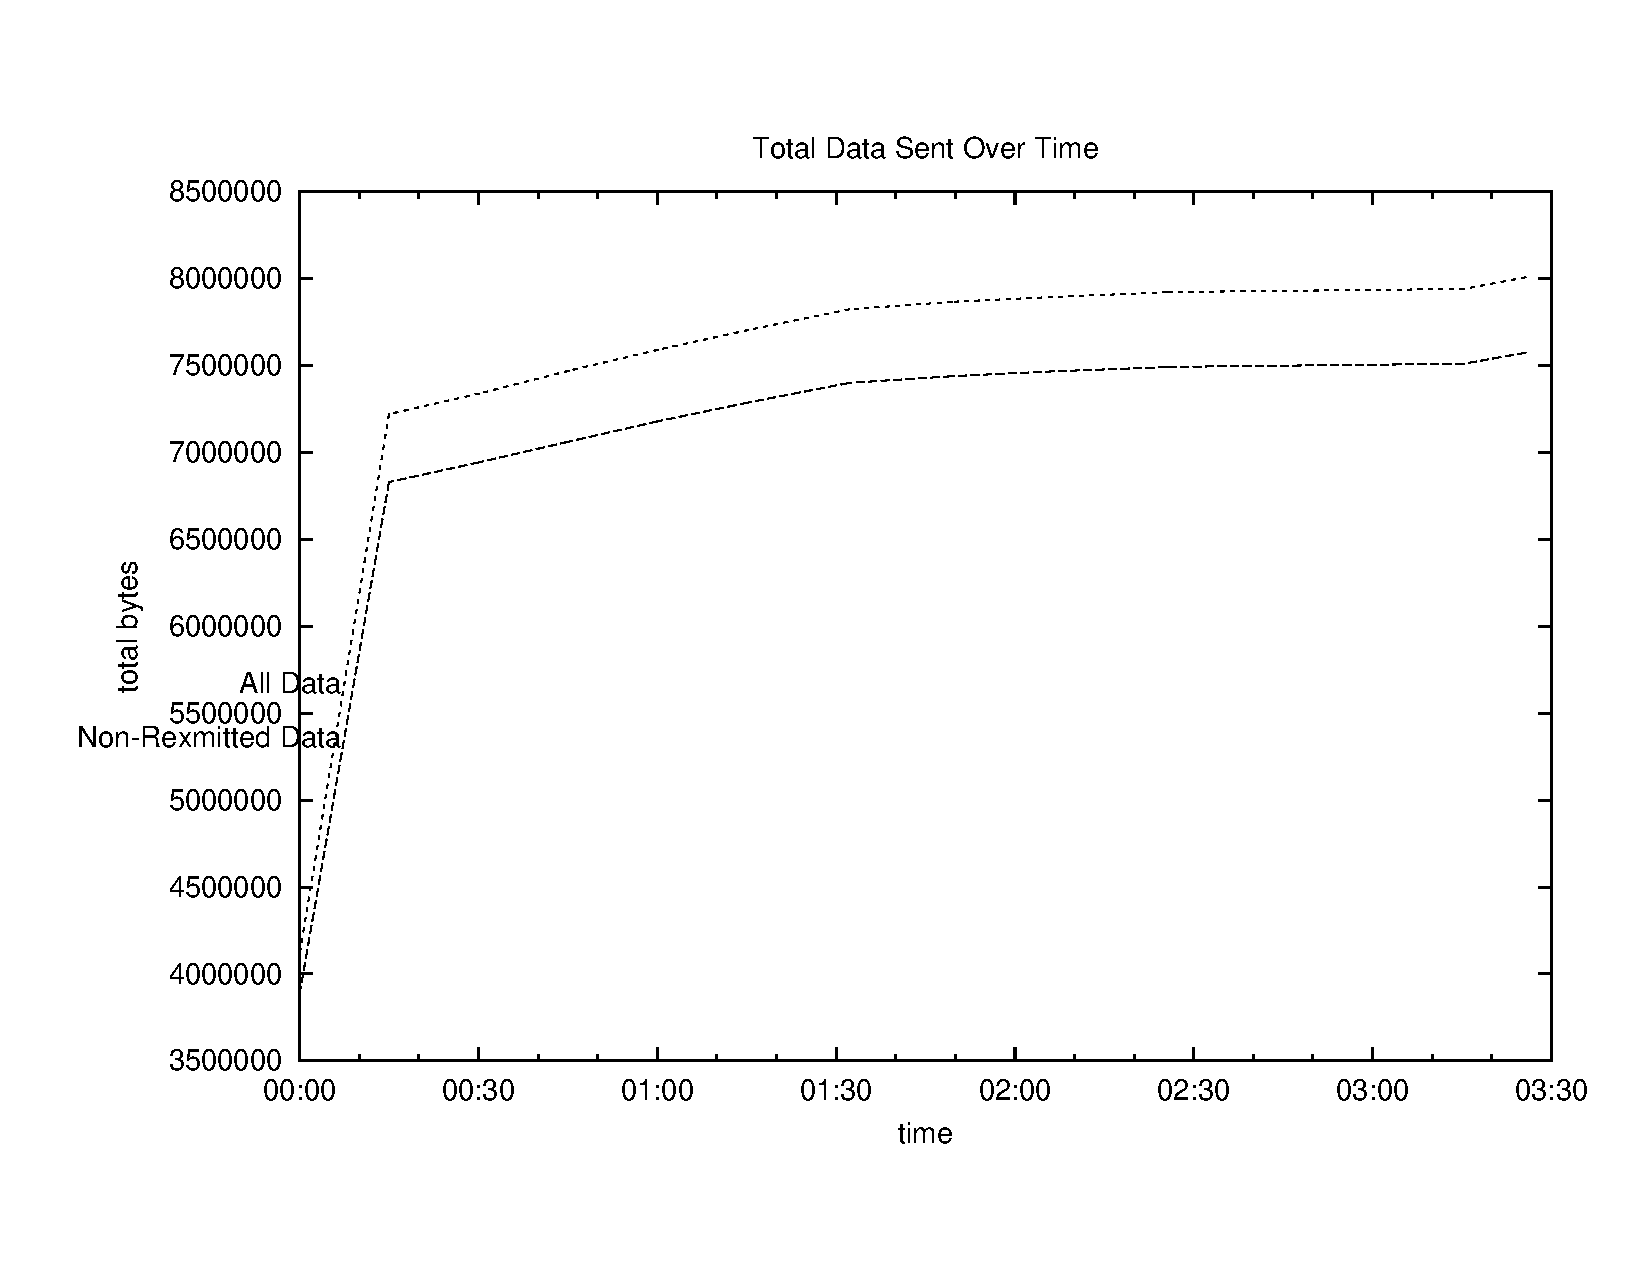
\includegraphics[width=\textwidth]{charts/dlna_traffic_5loss_data}
\end{minipage}
\begin{minipage}[b]{0.45\linewidth}
\centering
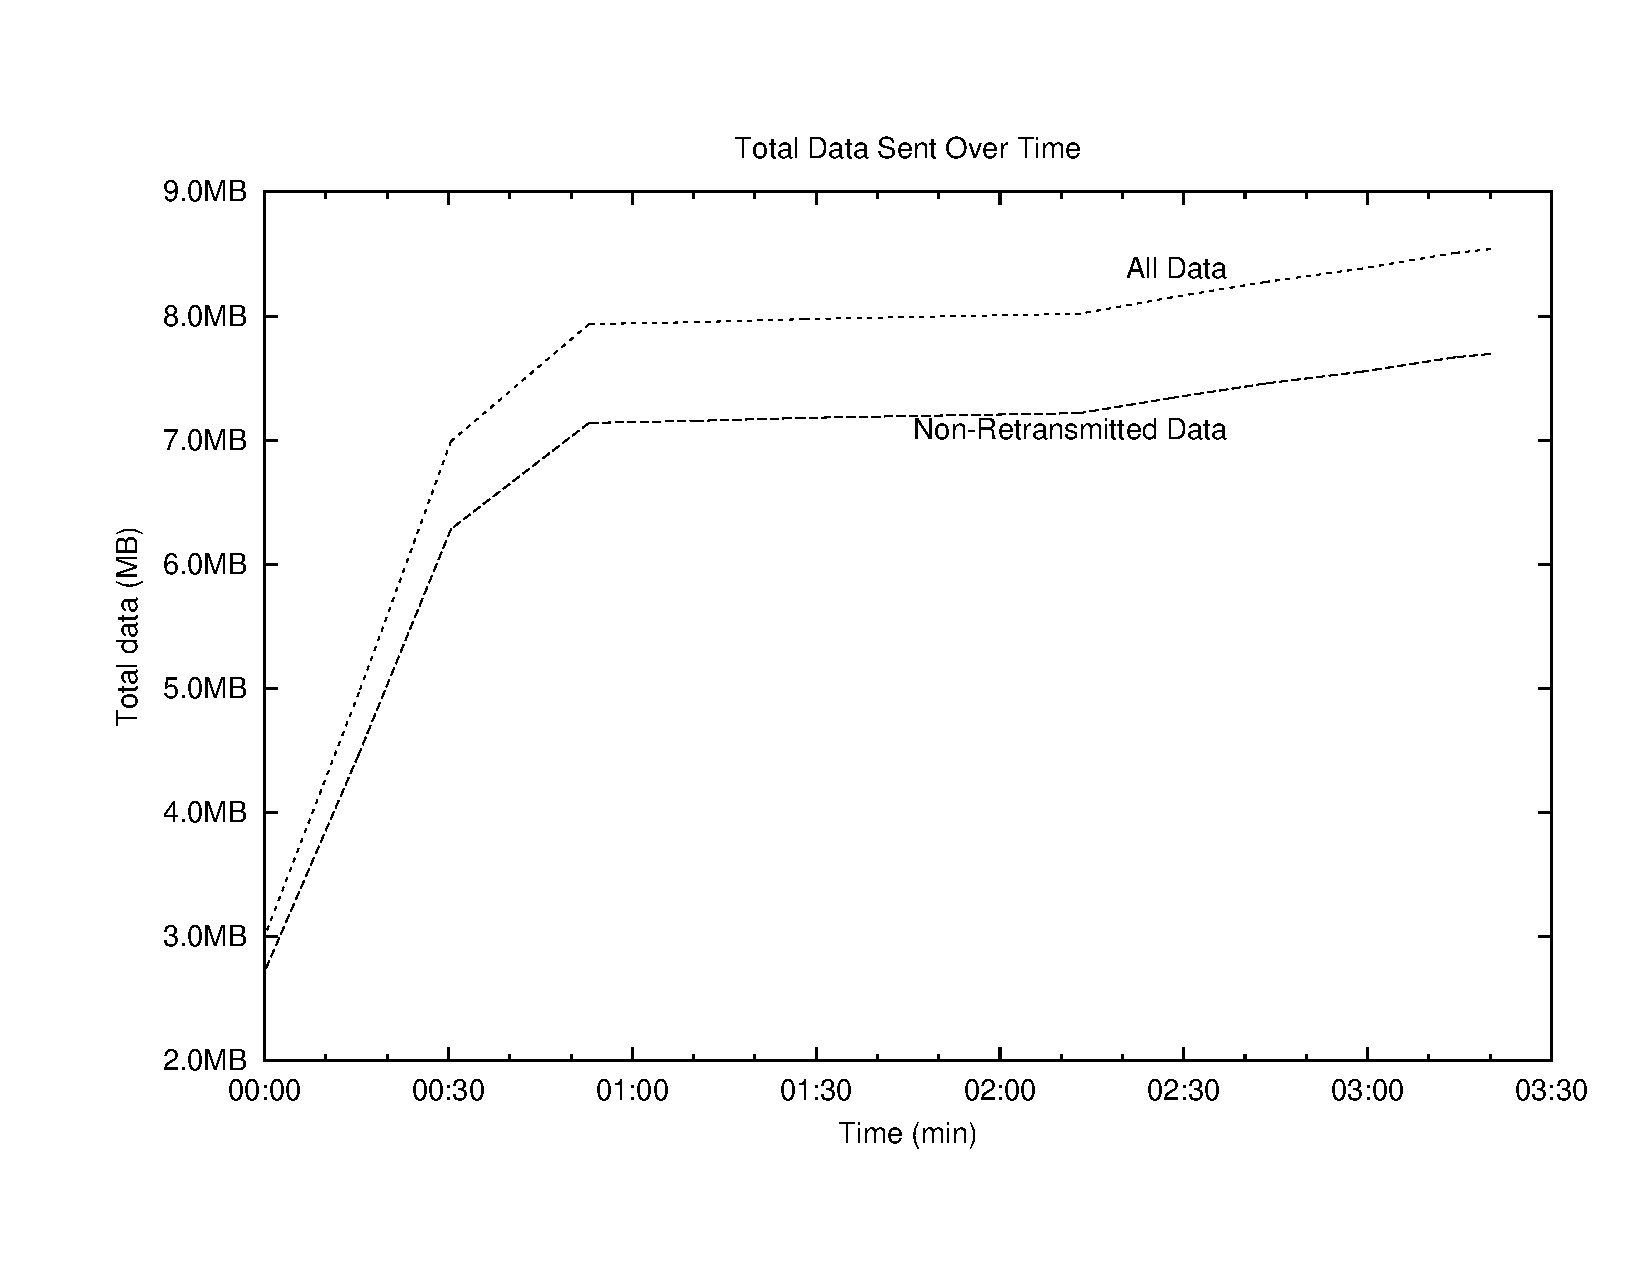
\includegraphics[width=\textwidth]{charts/dlna_traffic_10loss_data}
%%\hspace{0.1cm}
\end{minipage}
\begin{minipage}[b]{0.45\linewidth}
\centering
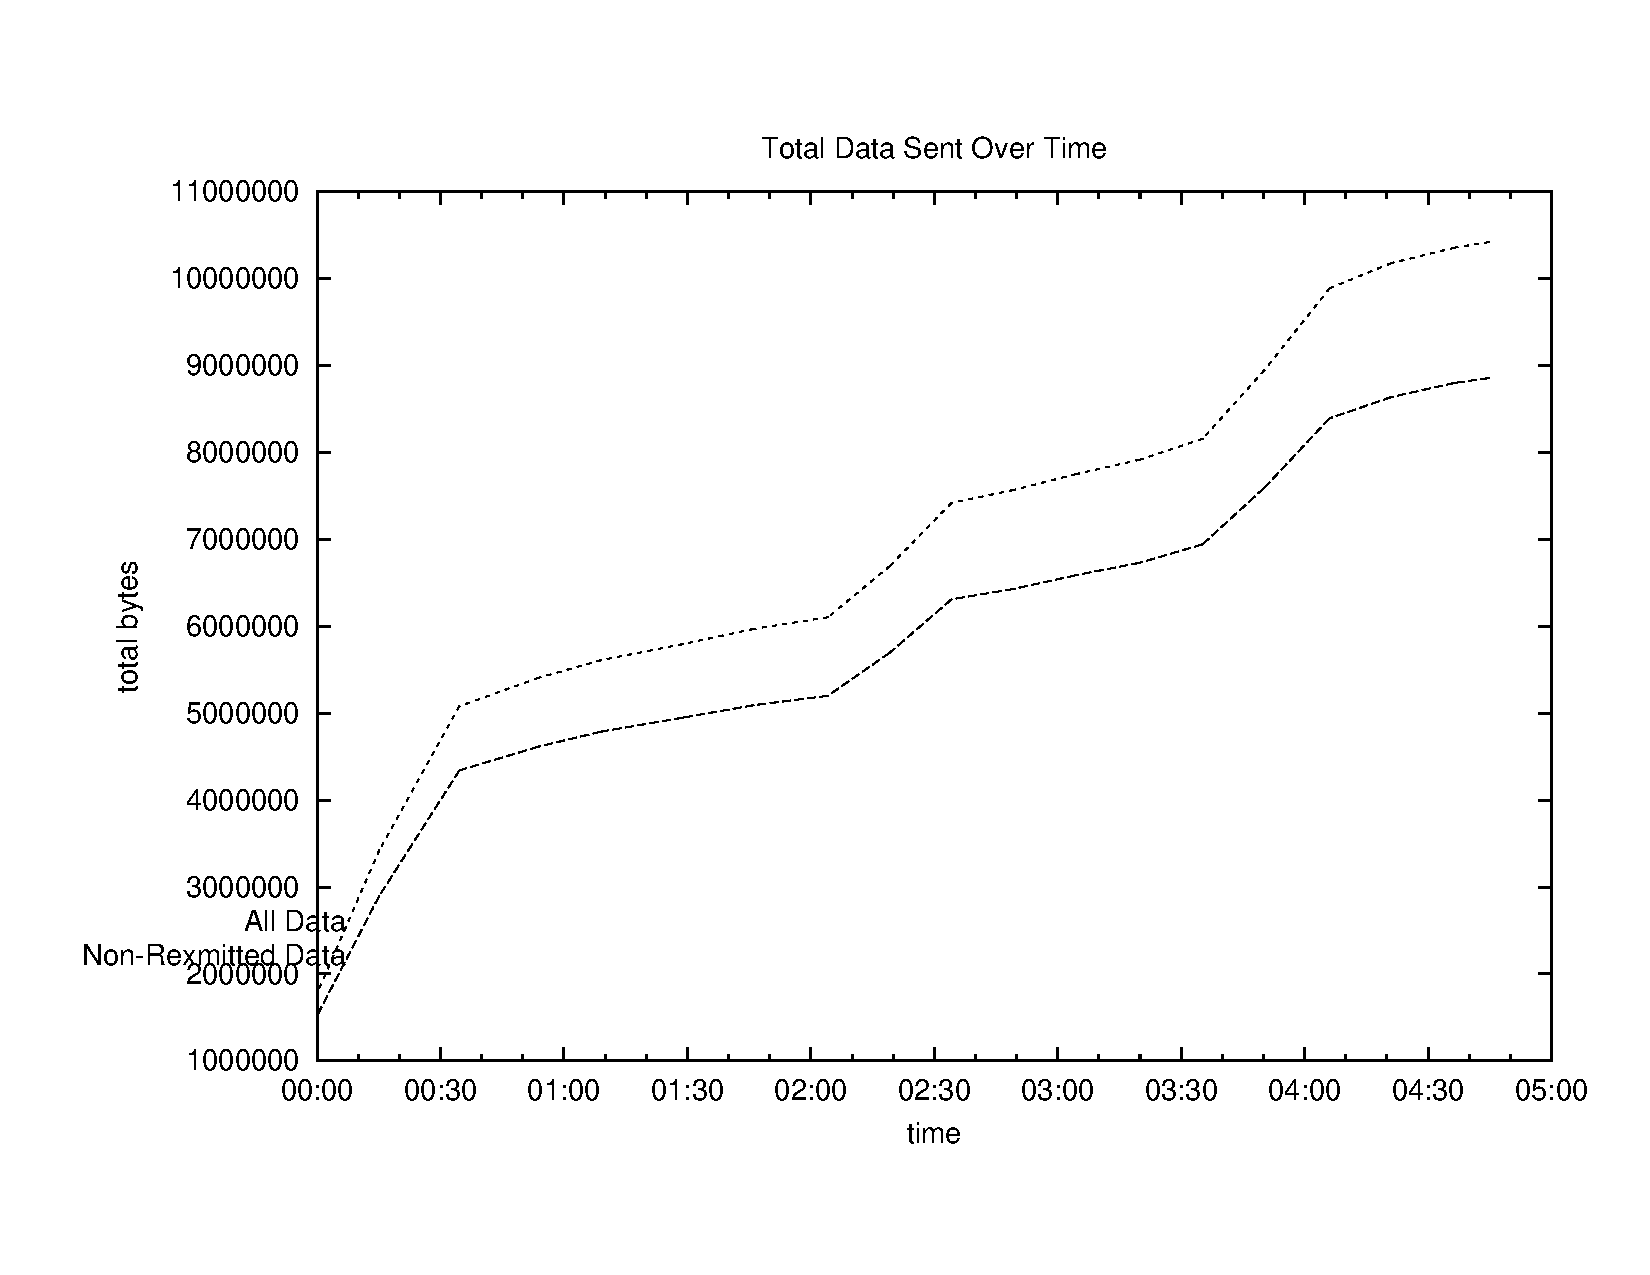
\includegraphics[width=\textwidth]{charts/dlna_traffic_15loss_data}
\end{minipage}
\caption{DLNA streaming performance in terms of packet loss}\label{multiavp}
\end{figure}

\begin{figure}[htb]
\centering 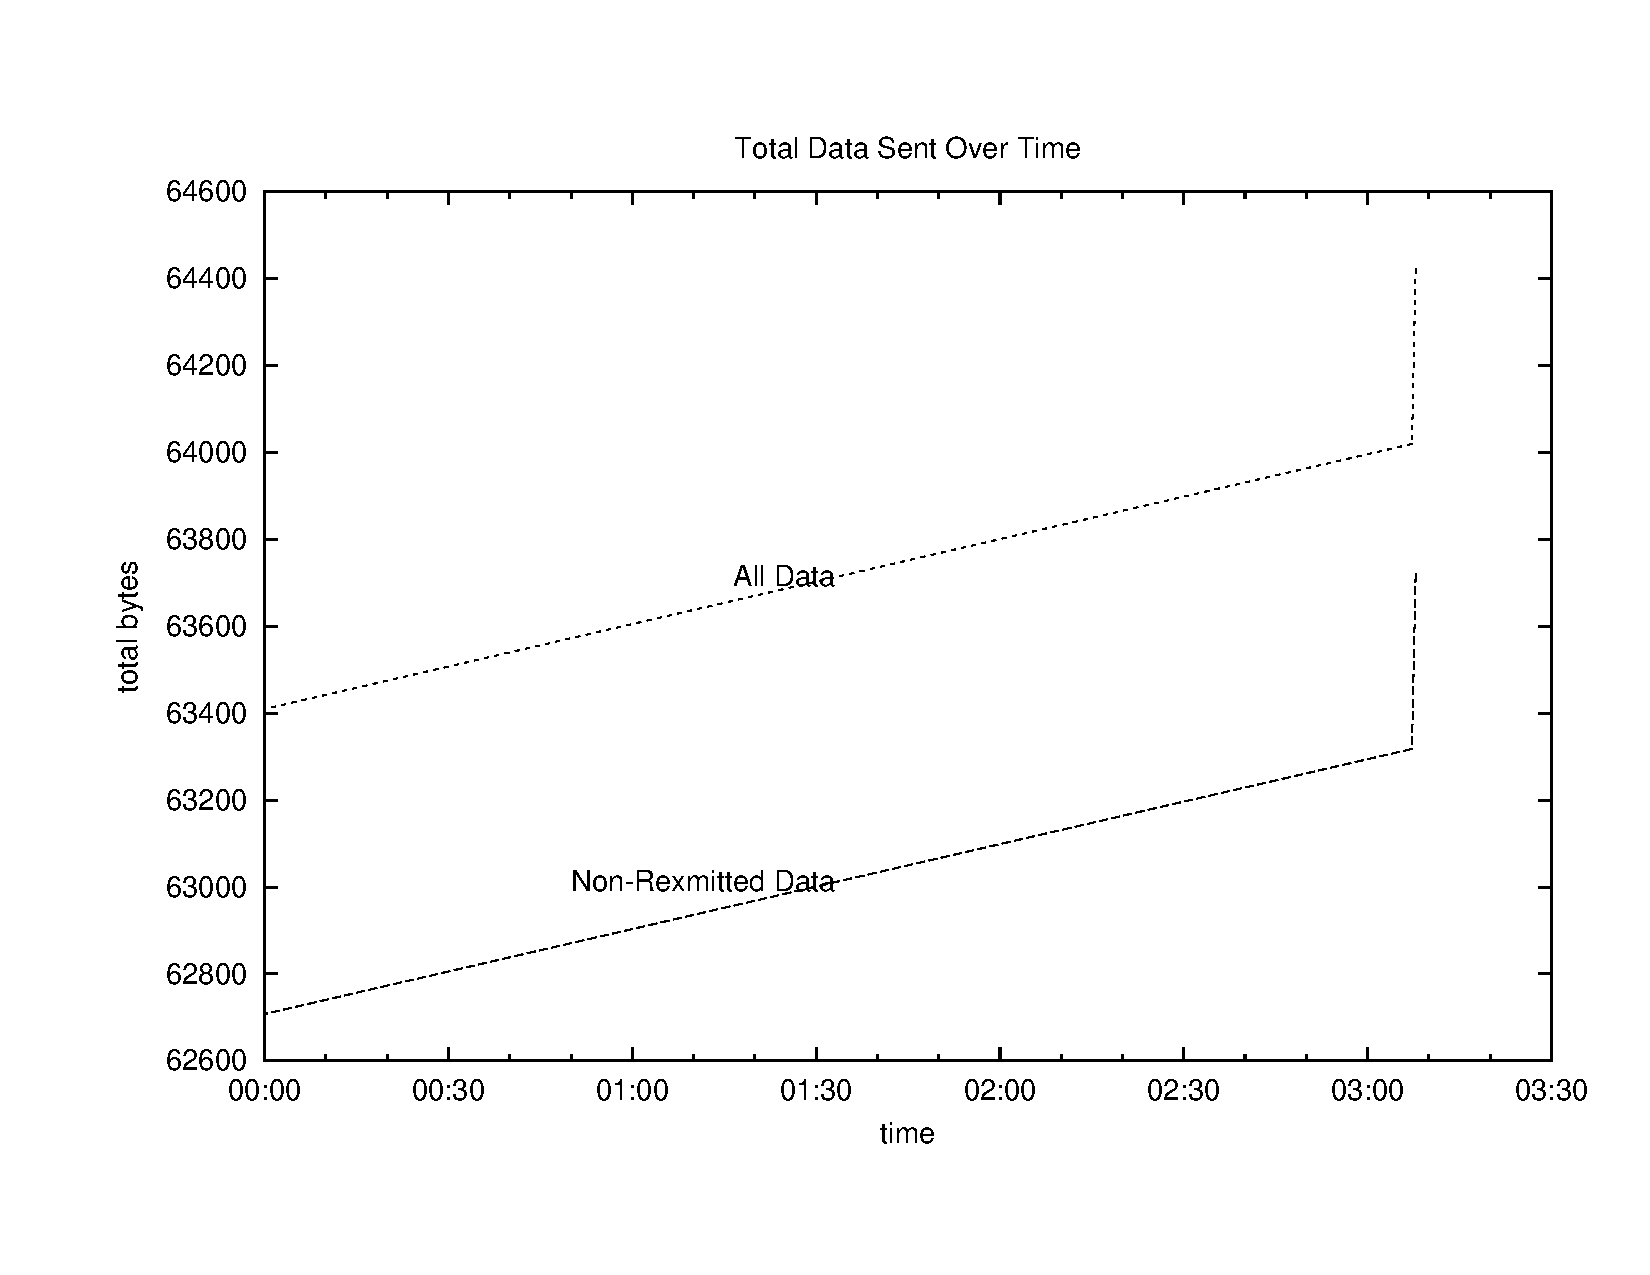
\includegraphics[height=10cm]{charts/airplay_traffic_data}
\caption{AirPlay traffic data chart \label{chart6}}
\end{figure}
\begin{figure}[htb]
\centering 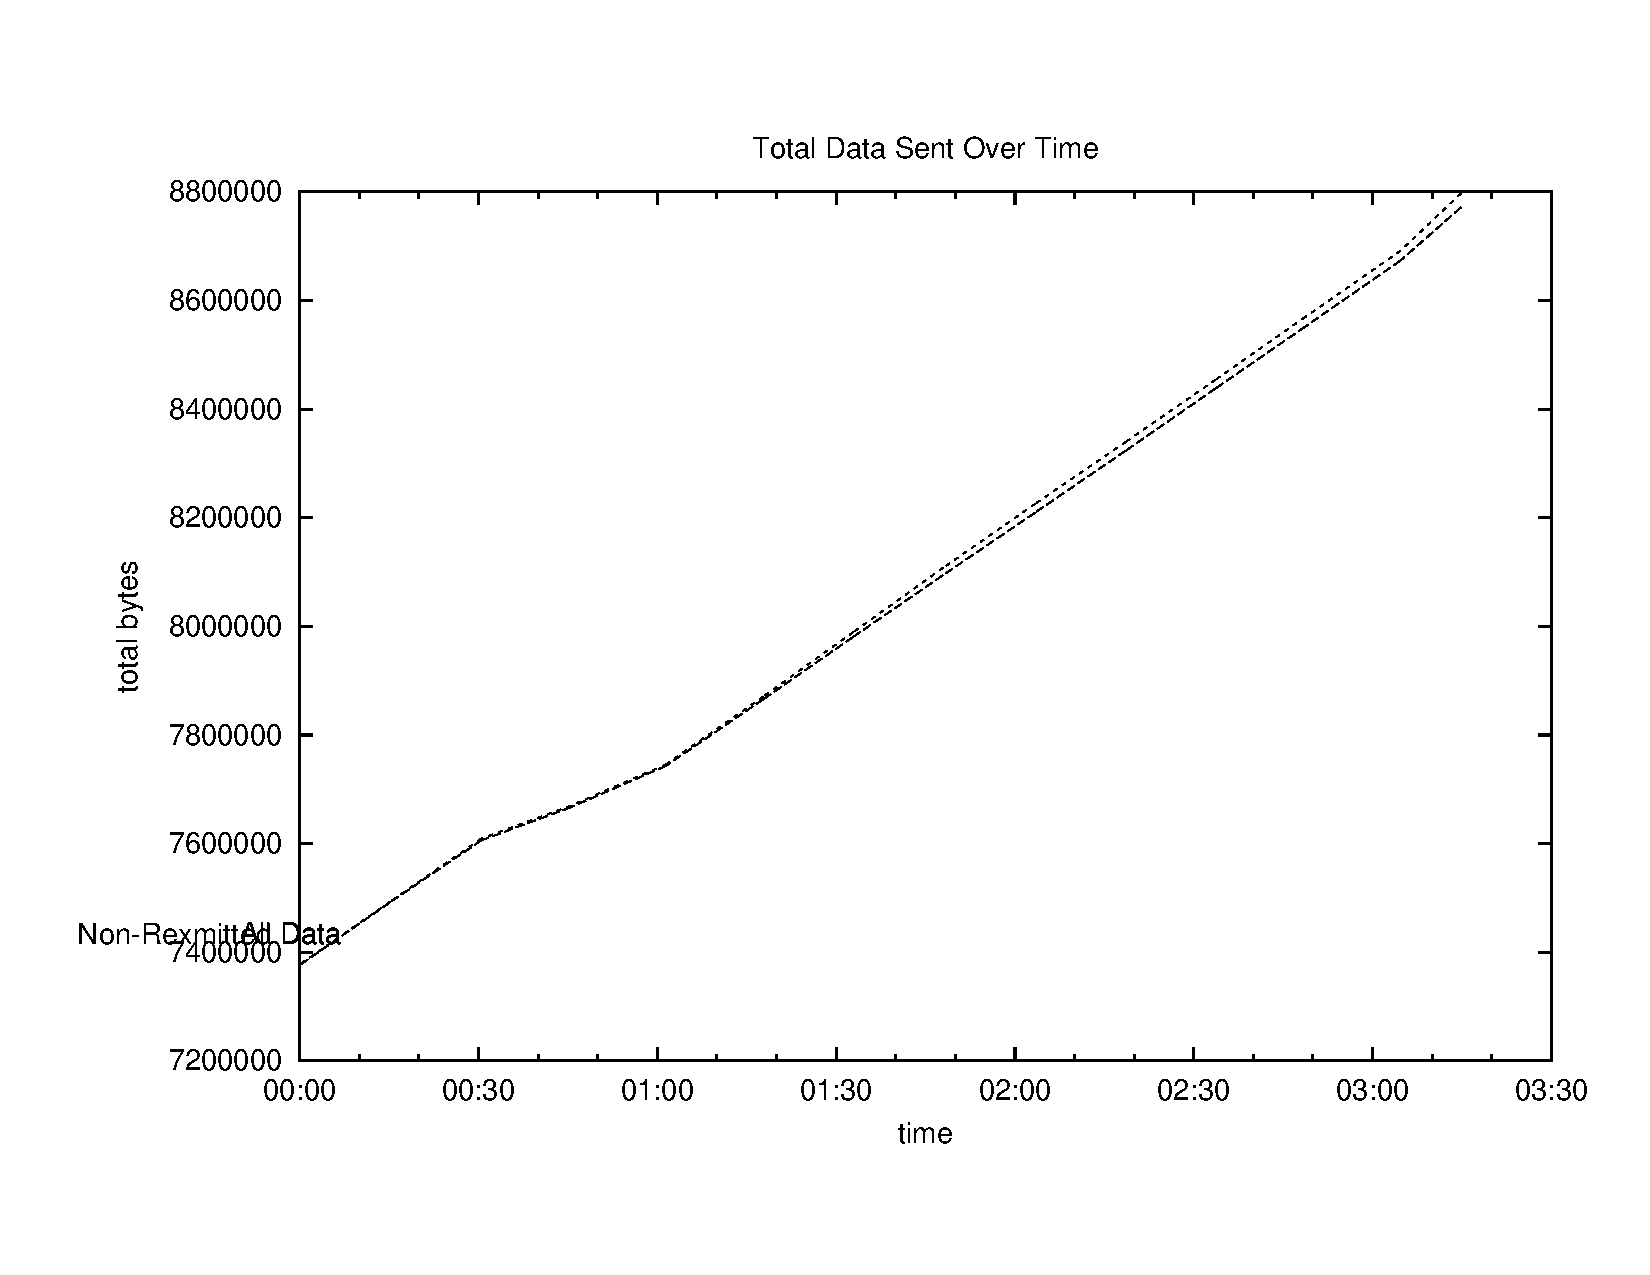
\includegraphics[height=10cm]{charts/dlna_traffic_data}
\caption{DLNA traffic data chart \label{chart6}}
\end{figure}

\begin{figure}[htb]
\centering 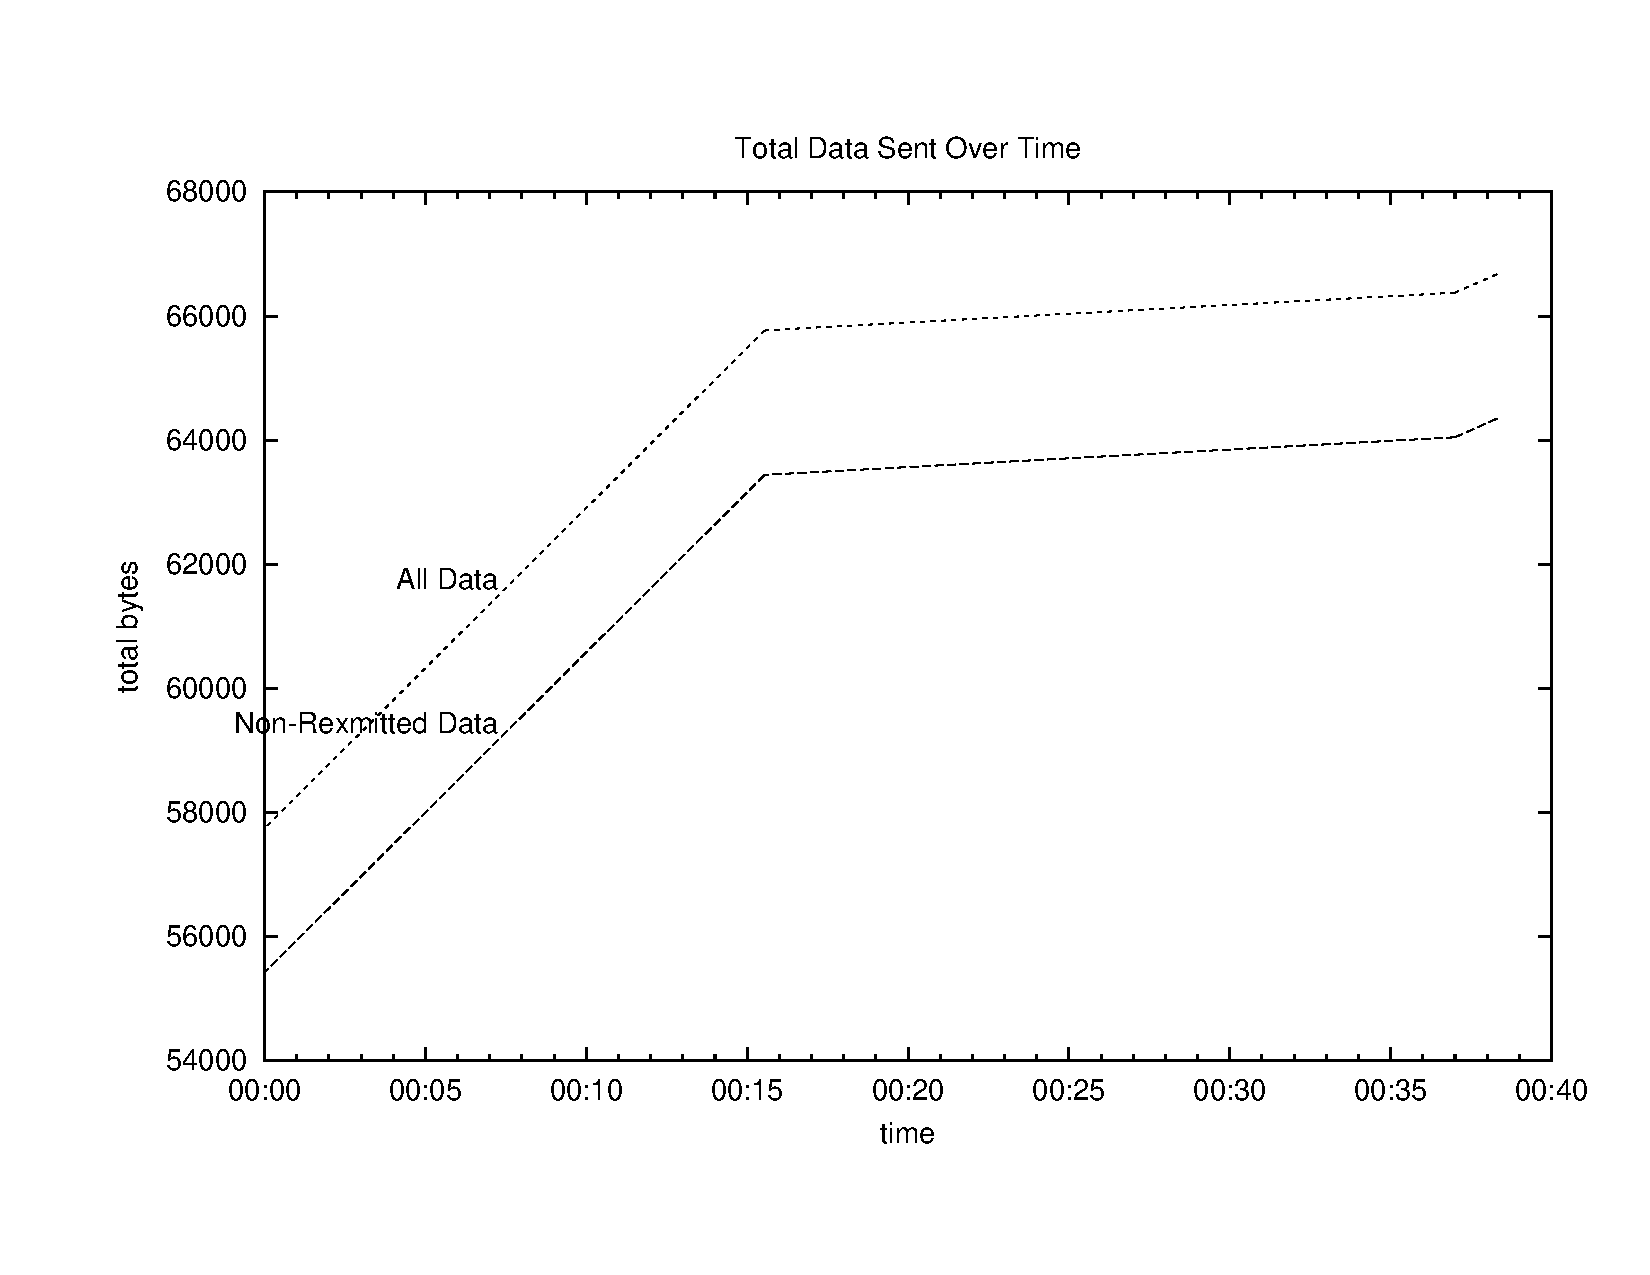
\includegraphics[height=10cm]{charts/badnetwork_airplay_traffic_data}
\caption{AirPlay bad network traffic data chart \label{chart6}}
\end{figure}
\begin{figure}[htb]
\centering 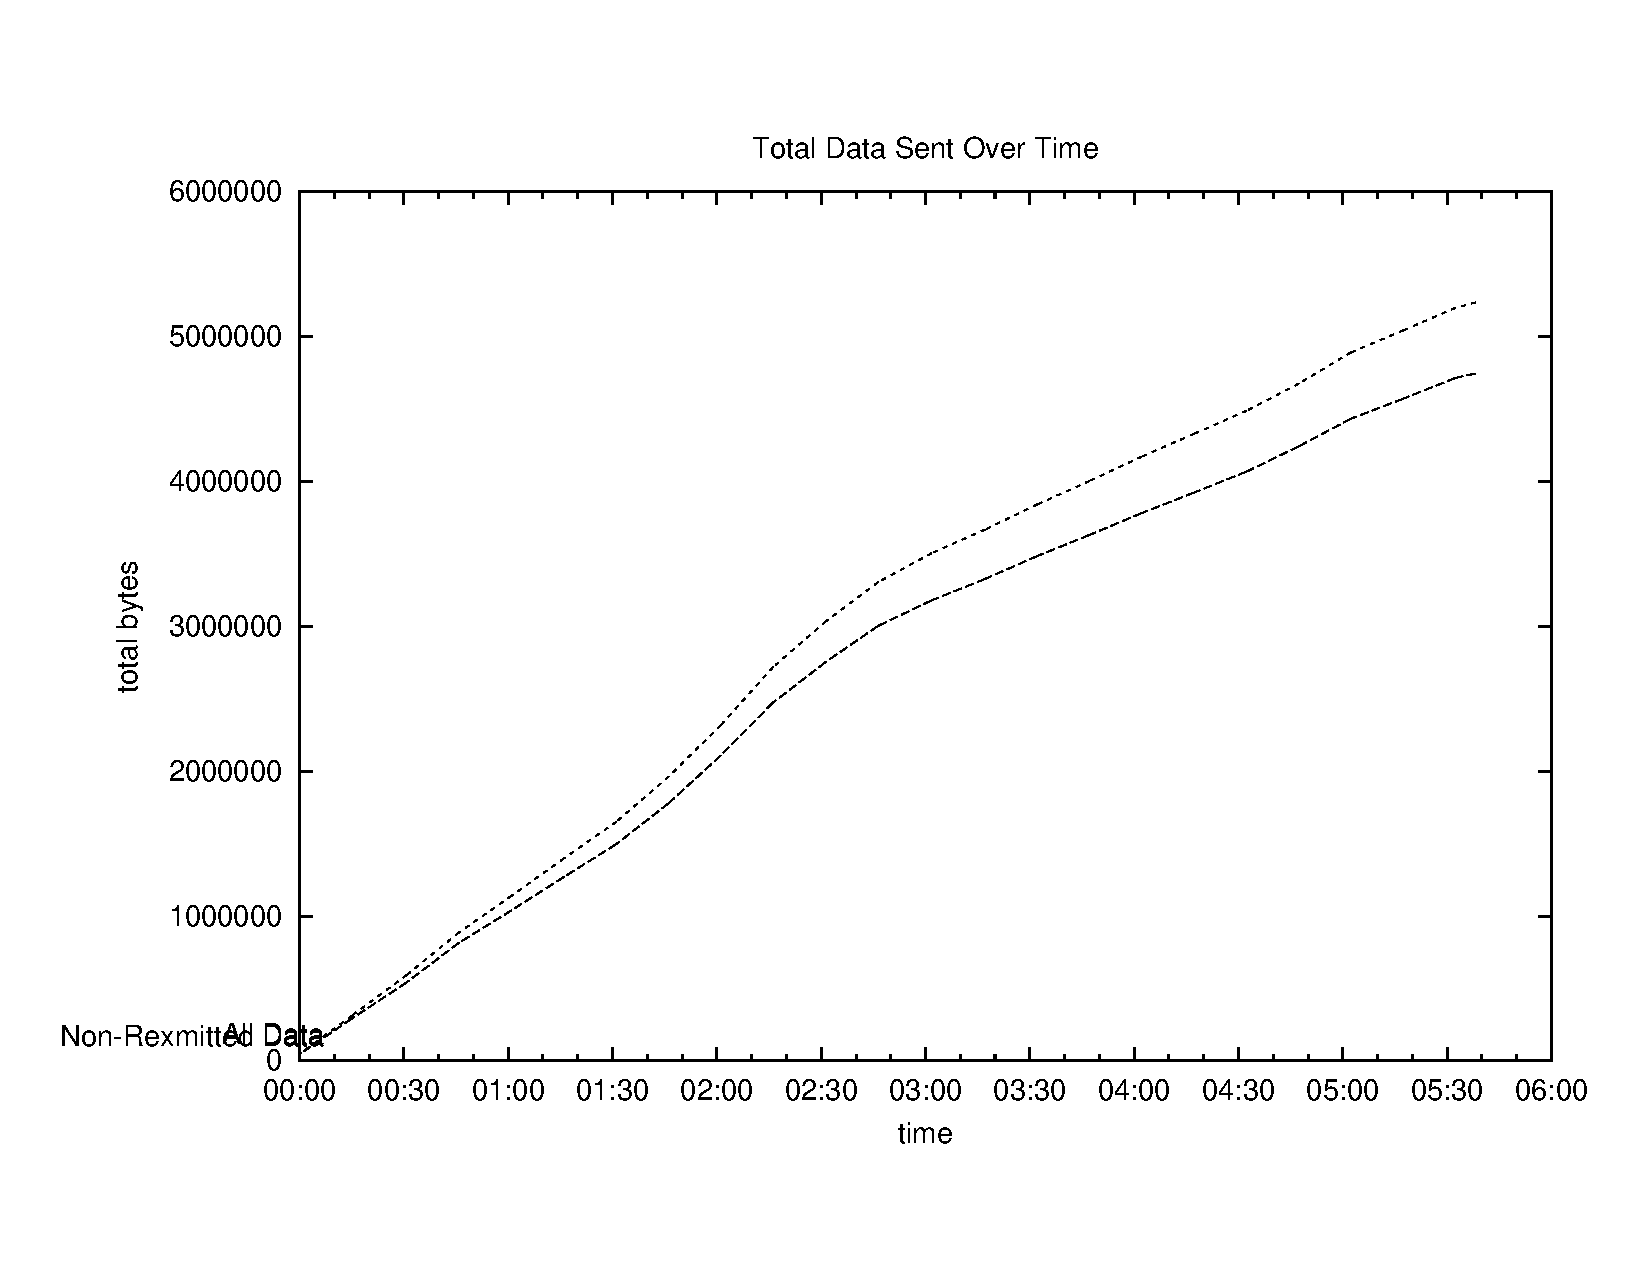
\includegraphics[height=10cm]{charts/badnetwork_dlna_traffic_data}
\caption{DLNA bad network traffic data chart \label{chart6}}
\end{figure}


\begin{figure}[htb]
\centering 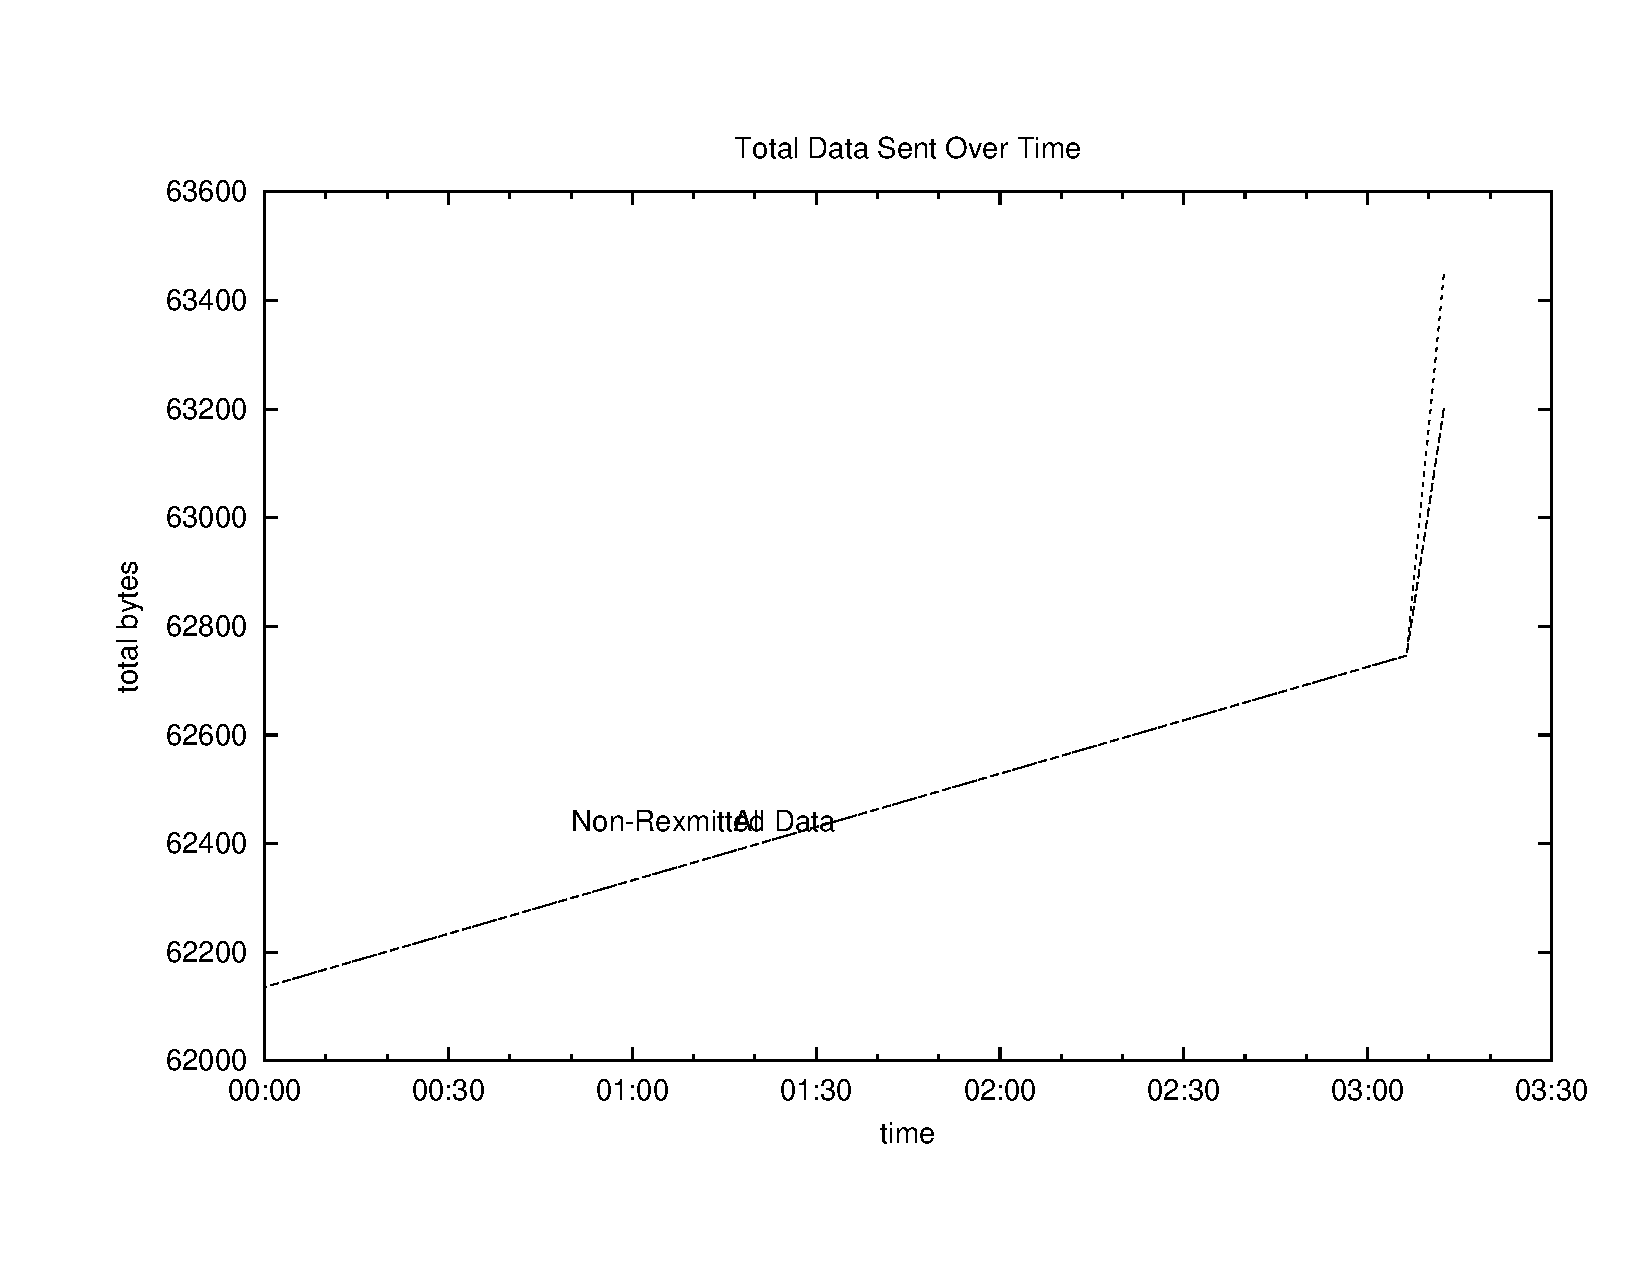
\includegraphics[height=10cm]{charts/airplay_traffic_5loss_data}
\caption{AirPlay bad network traffic data chart \label{chart6}}
\end{figure}
\begin{figure}[htb]
\centering 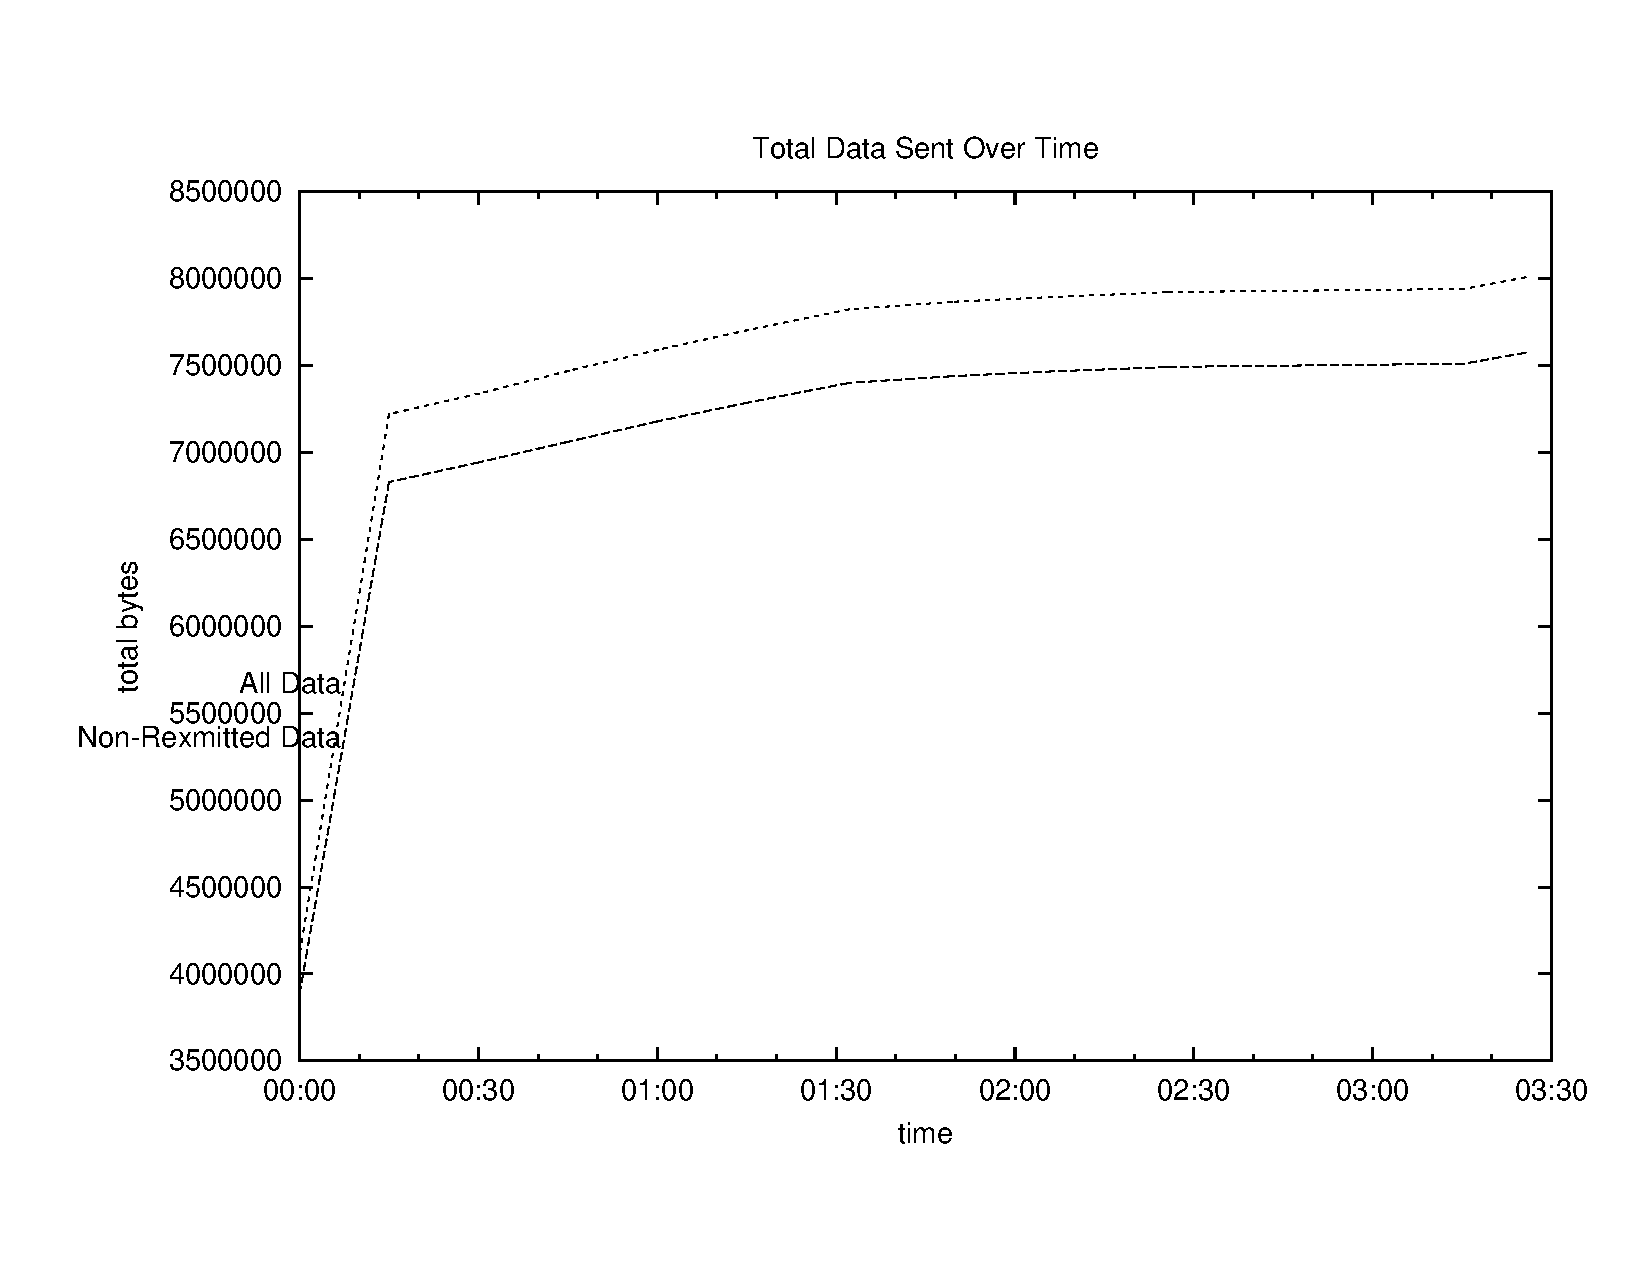
\includegraphics[height=10cm]{charts/dlna_traffic_5loss_data}
\caption{DLNA bad network traffic data chart \label{chart6}}
\end{figure}


\begin{figure}[htb]
\centering 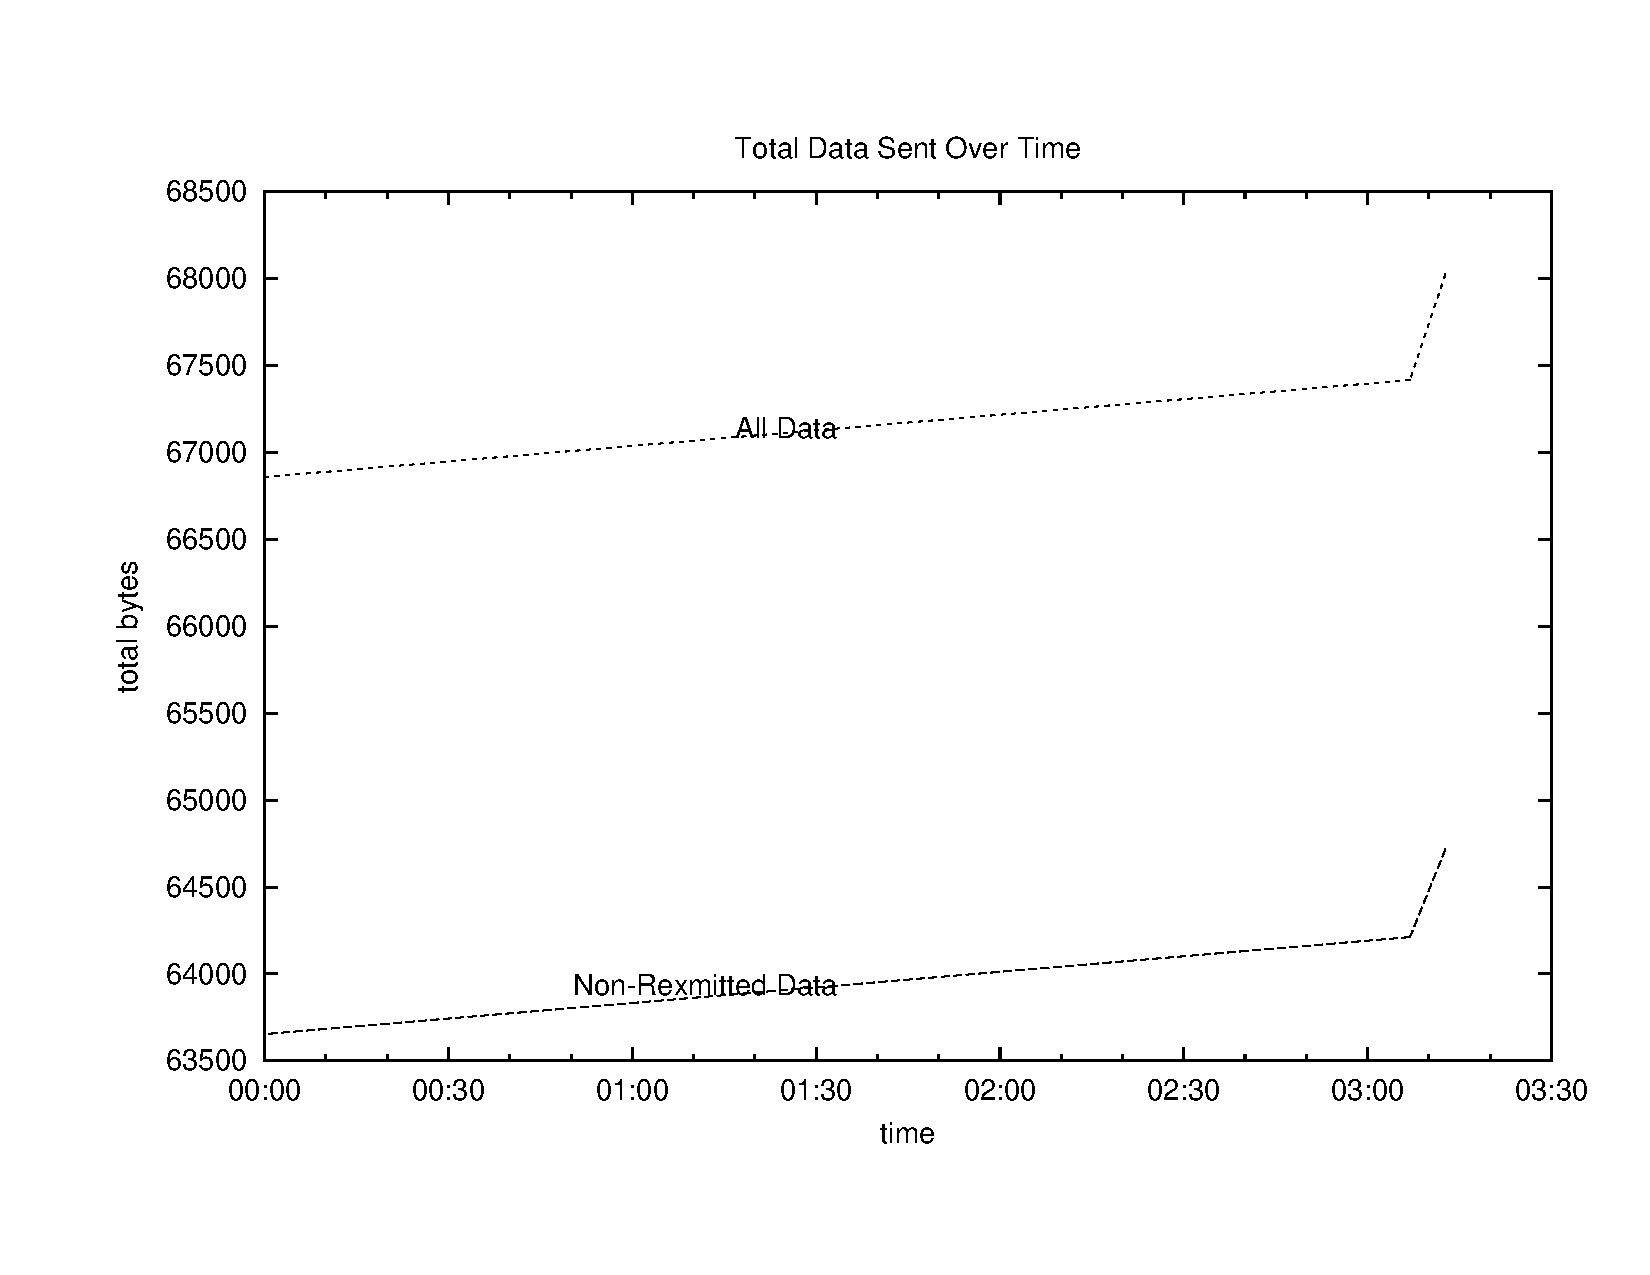
\includegraphics[height=10cm]{charts/airplay_traffic_10loss_data}
\caption{AirPlay bad network traffic data chart \label{chart6}}
\end{figure}
\begin{figure}[htb]
\centering 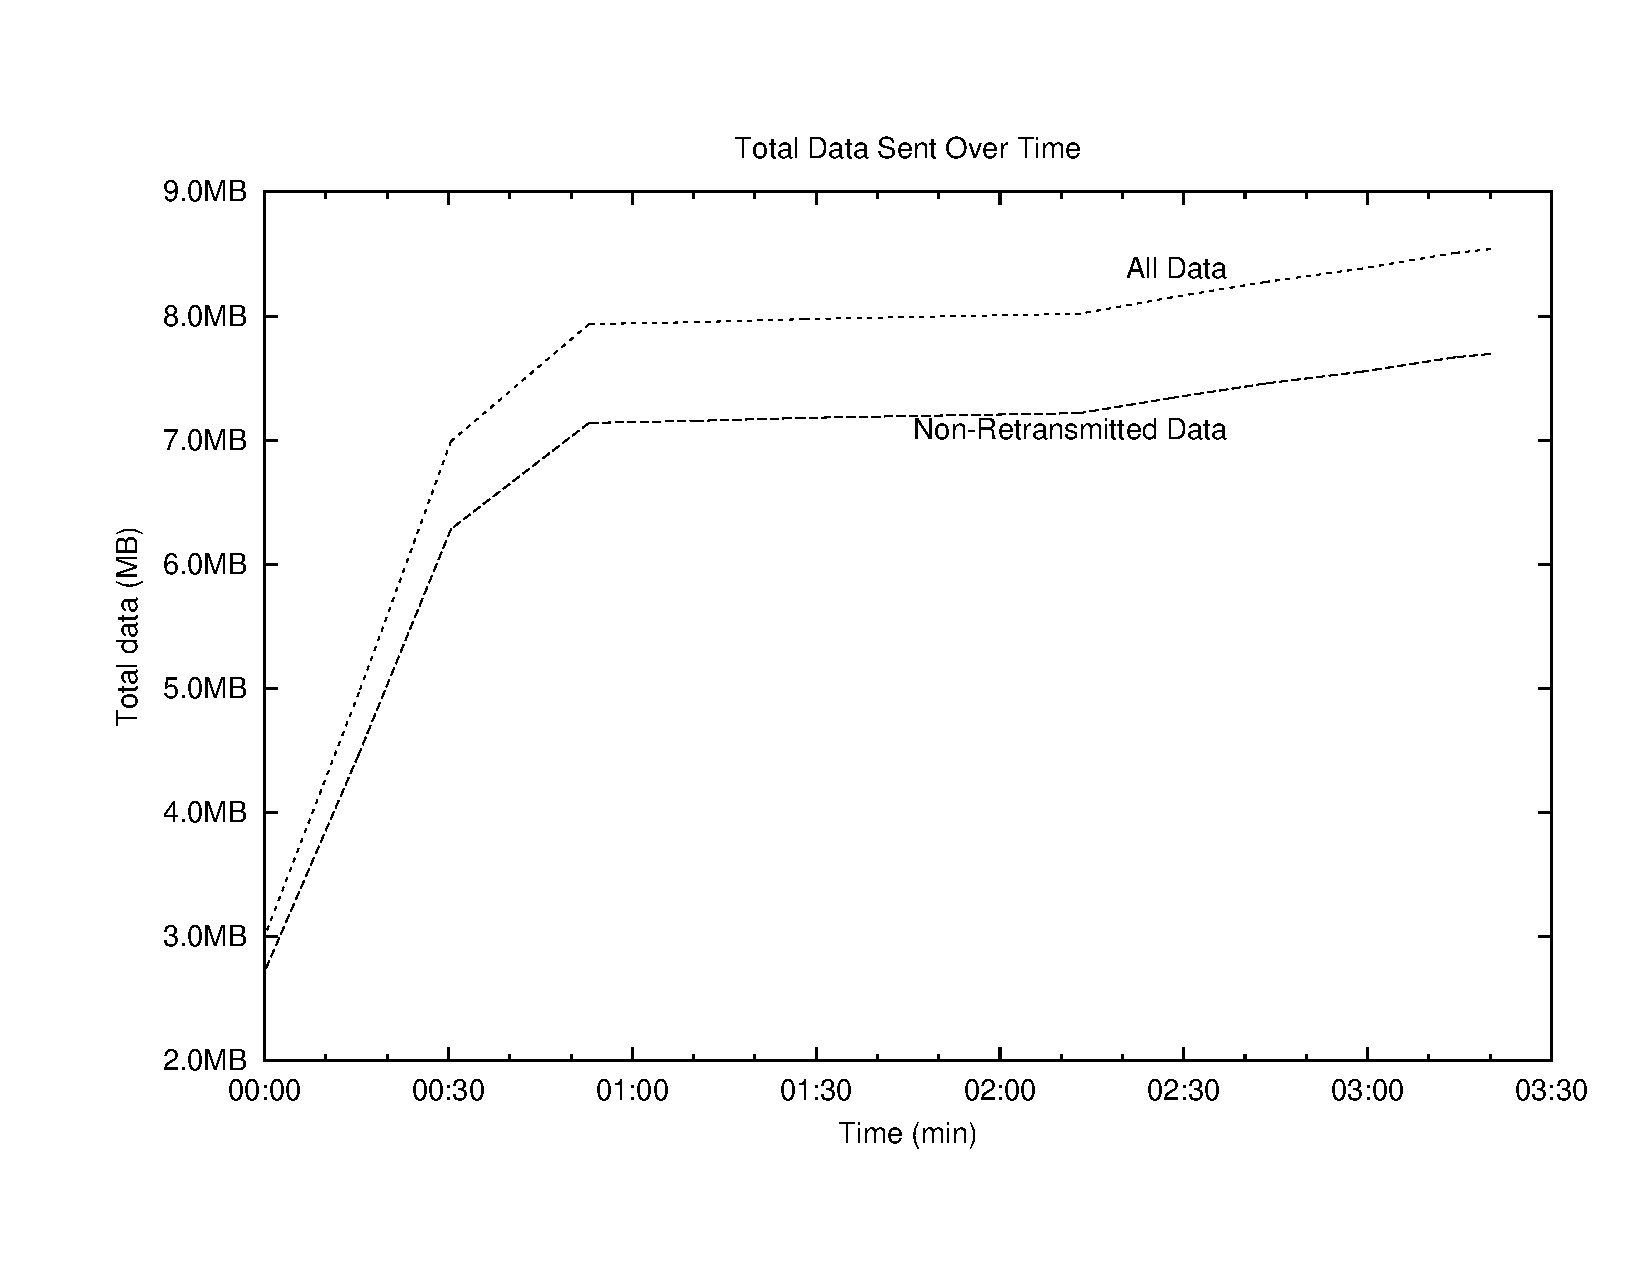
\includegraphics[height=10cm]{charts/dlna_traffic_10loss_data}
\caption{DLNA bad network traffic data chart \label{chart6}}
\end{figure}


\begin{figure}[htb]
\centering 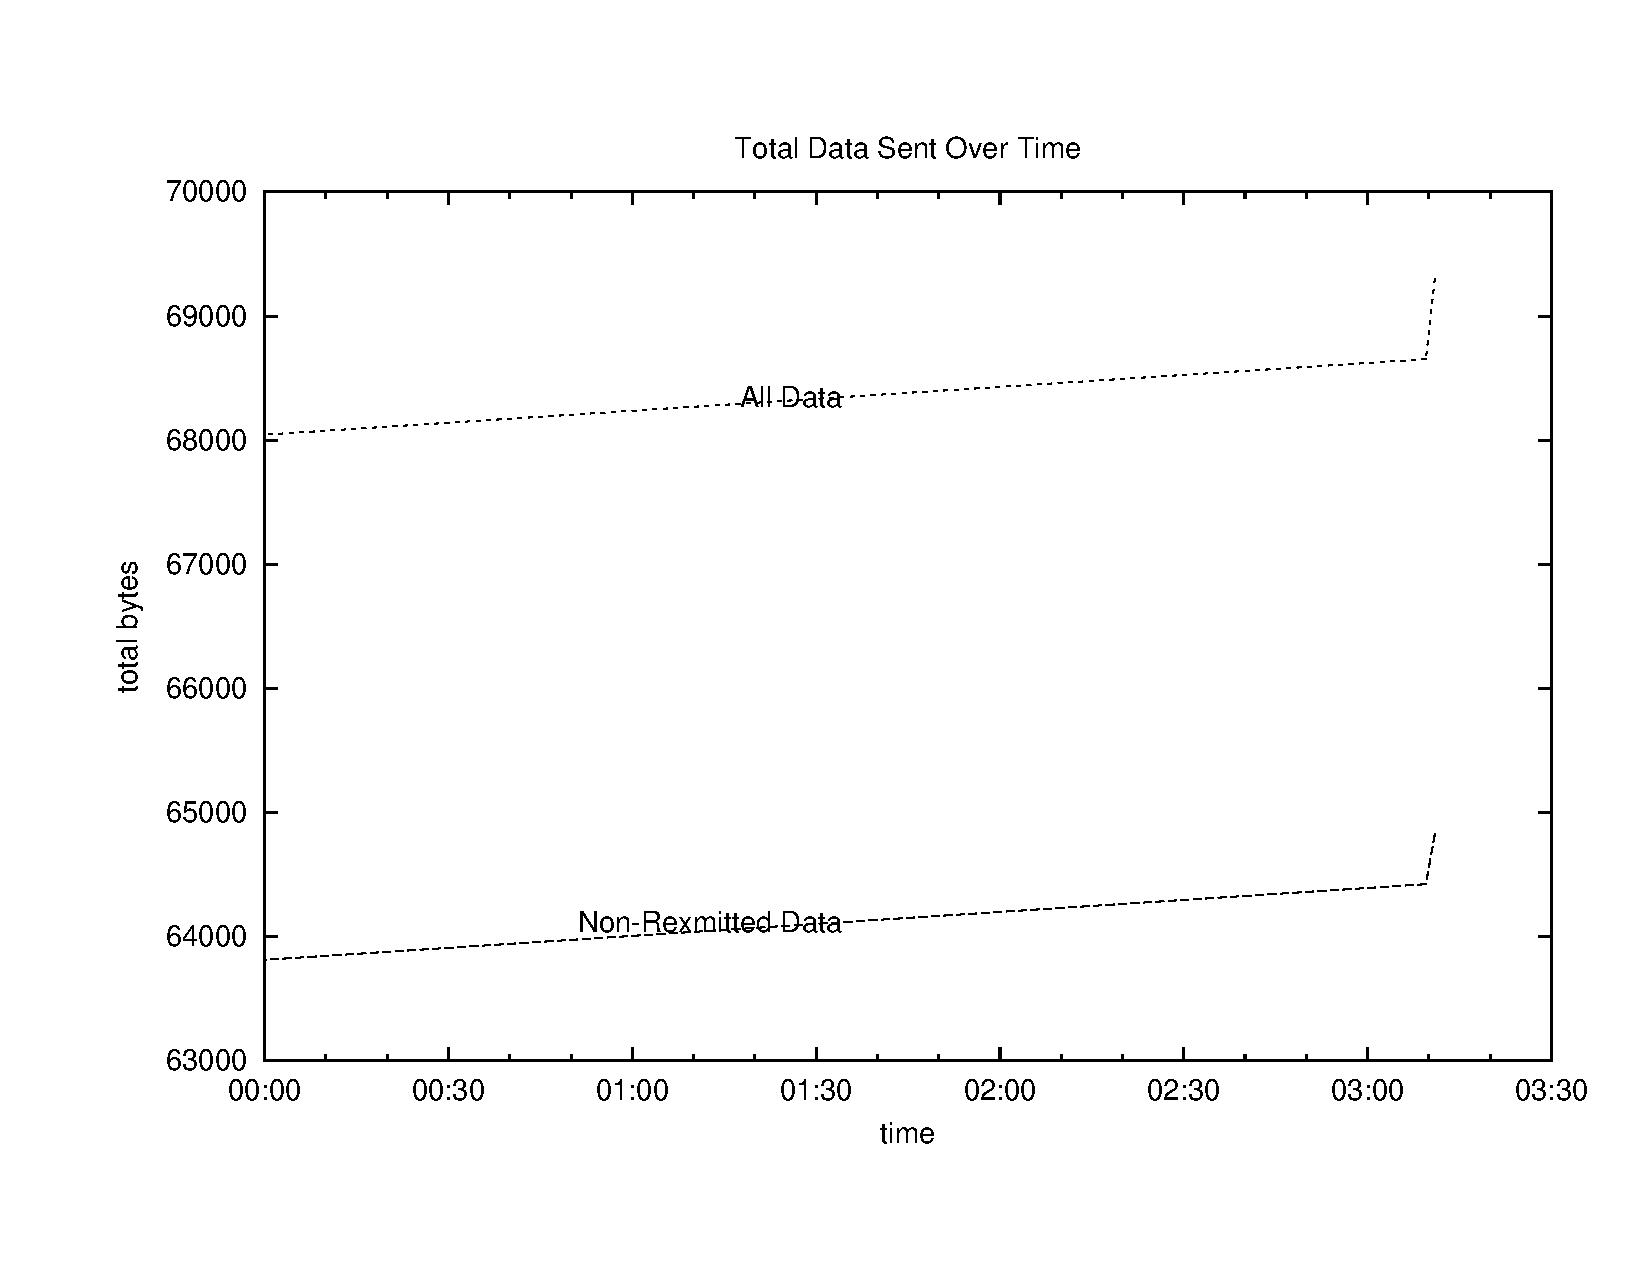
\includegraphics[height=10cm]{charts/airplay_traffic_15loss_data}
\caption{AirPlay bad network traffic data chart \label{chart6}}
\end{figure}
\begin{figure}[htb]
\centering 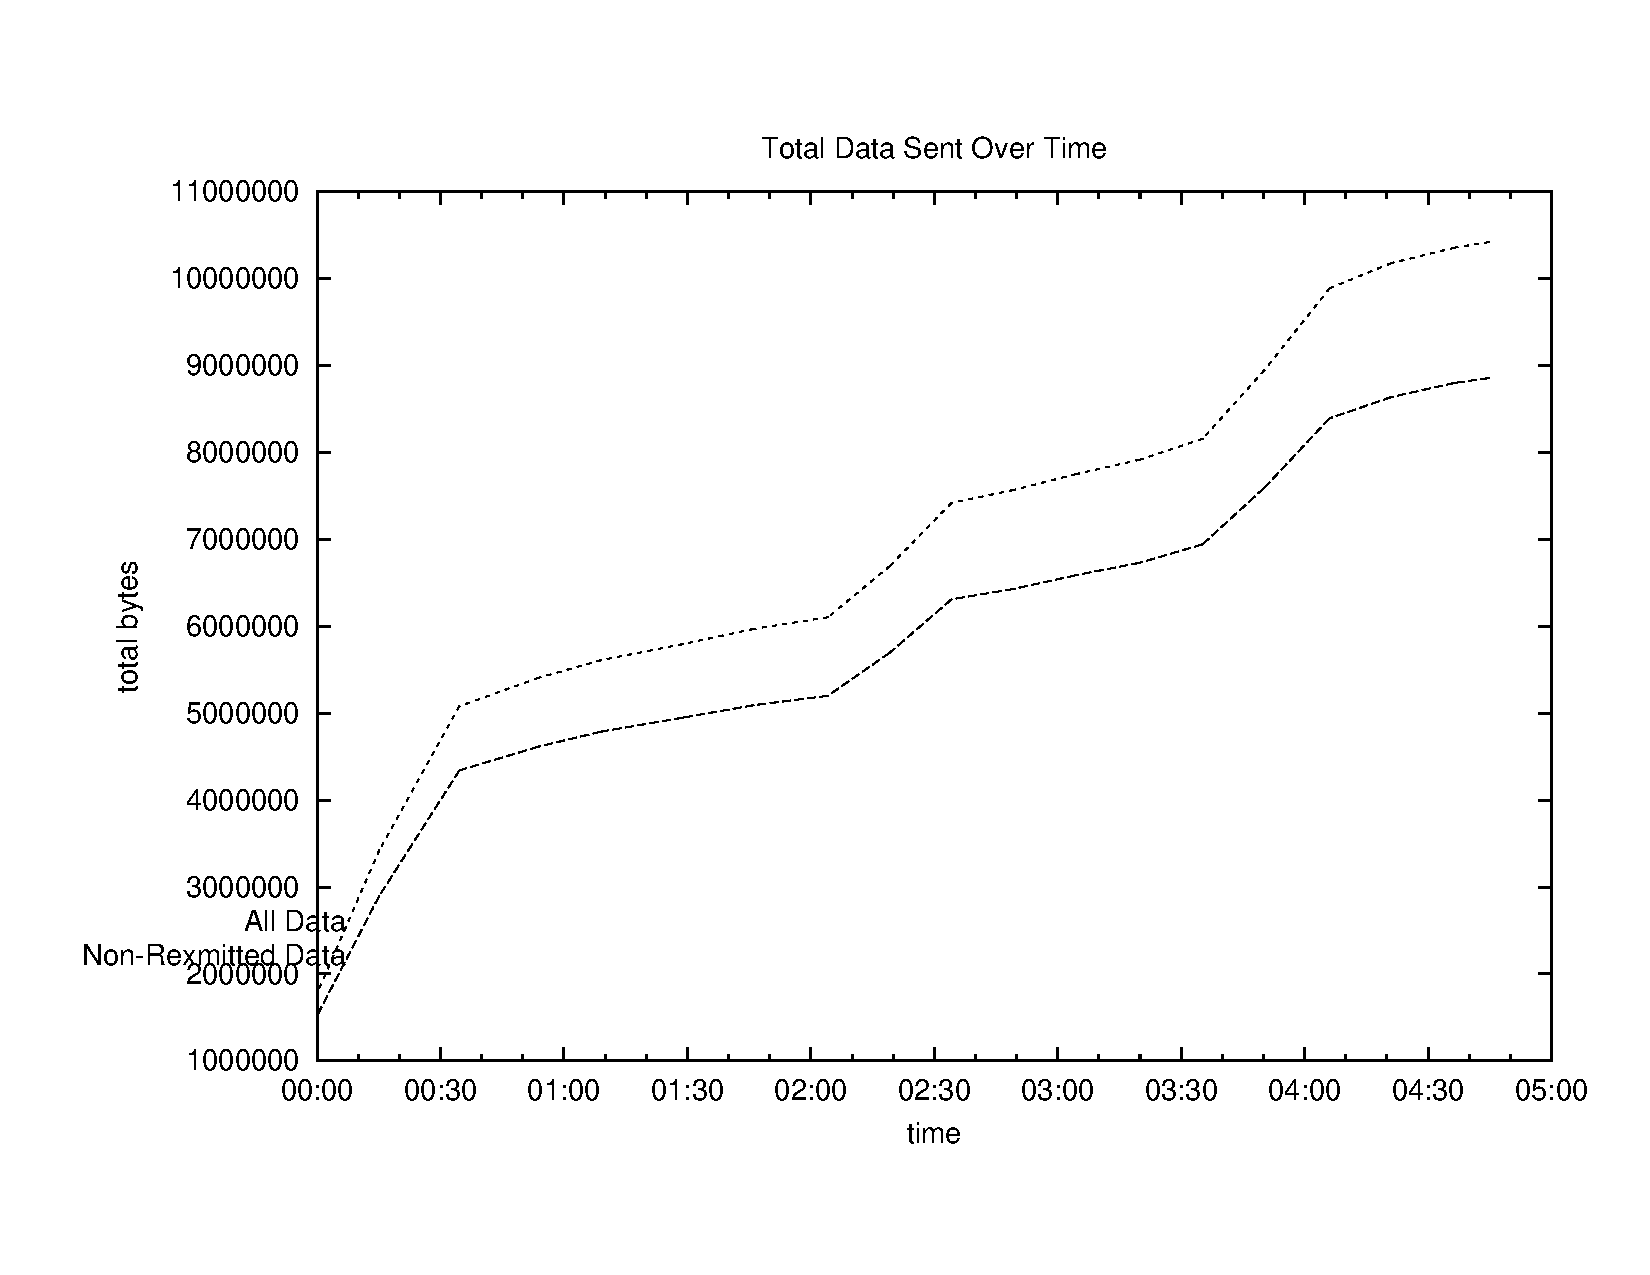
\includegraphics[height=10cm]{charts/dlna_traffic_15loss_data}
\caption{DLNA bad network traffic data chart \label{chart6}}
\end{figure}

\subsection{Statistics}
Through one year's on-line marketing, we reached 637000 downloads from 223
countries all around the world, with around 8000 daily active users. So far, the
average rating of our app is 3.9 out of 7527 ratings. The application turns out
to be popular in countries like France, United States, Germany, United Kingdom
and Brazil.

\begin{itemize}
\item[--]Totally more than 290000 downloads
\item[--]Used by people from 201 countries
\item[--]8000+ daily active users
\item[--]1,241,074 visits to home page
\item[--]Average rating 3.9, 3521 user gave rates
\item[--]On-line for 3 months
\end{itemize}
\begin{figure}[htb]
\centering 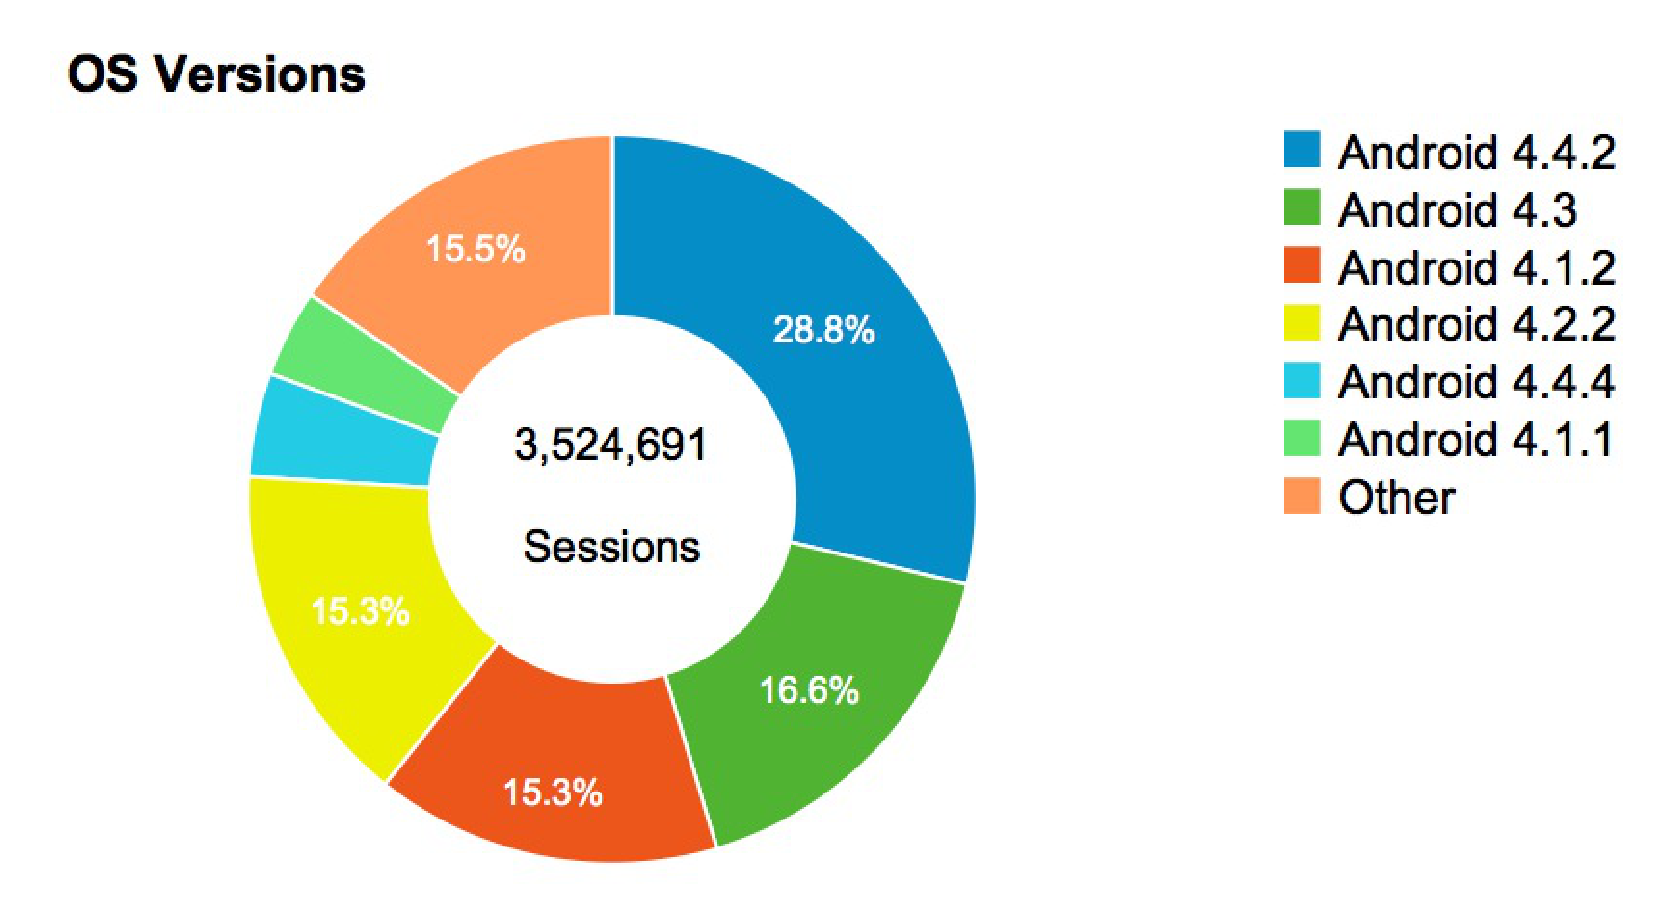
\includegraphics[height=5cm]{charts/android_versions}
\caption{Android versions \label{chart6}}
\end{figure}

\begin{figure}[htb]
\centering \includegraphics[height=9cm]{charts/user_world_map}
\caption{User world map \label{chart7}}
\end{figure}

\begin{table}[htb]
\caption{Receiver type statistic \label{Table8}}
\begin{center}
\fbox{
\begin{tabular}{c|l|l}  
\textbf{Device type } & Total selection & Percentage \\
\hline \textbf{AirPlay device} & 637446 & 39.72\\ \hline
\textbf{DLNA device} & 460139 & 28.67\\ \hline
\textbf{Phone speaker} & 353474 & 22.03\\ \hline
\textbf{Chromecast device} & 147333 & 9.18\\ \hline
\textbf{FireTV device} & 6368 & 0.40
\end{tabular}
}
\end{center}
\end{table}

\subsection{User study}
\begin{itemize}
\item[--]What information we can get back from users
\item[--]User behavior/ statistics
\item[--]Improve the application accordingly
\item[--]Strategies for decision making
\end{itemize}
Write result here.

\clearpage
\vspace*{100px}
\section{Summary\label{chapter5}}

%% Discussion chapter
%% author Liu Peng

Write discussion here.

\clearpage

%% L�hdeluettelo
%%
%% \phantomsection varmistaa, ett� hyperref-paketti latoo hypertekstilinkit
%% oikein.
%%
%% The \phantomsection command is nessesary for hyperref to jump to the 
%% correct page, in other words it puts a hyper marker on the page.

\phantomsection
%\addcontentsline{toc}{section}{Viitteet}
\addcontentsline{toc}{section}{References}

\bibliographystyle{unsrt}
\bibliography{reference} 

%\begin{thebibliography}{99}
%%% Reference chapter
%% author Liu Peng

%% Alla pilkun j�lkeen on pakotettu oikea v�li \<v�lily�nti>-merkeill�.
\bibitem{Kauranen} Kauranen,\ I., Mustakallio,\ M. ja Palmgren,\ V.
  \textit{Tutkimusraportin kirjoittamisen opas 
    .}  Espoo, Teknillinen korkeakoulu, 2006.

\bibitem{Itkonen} Itkonen,\ M. \textit{Typografian .} 3.\
  painos.  Helsinki, RPS-yht, 2007.

\bibitem{Koblitz} Koblitz,\ N. \textit{A Course in Number Theory and
    Cryptography. Graduate Texts in Mathematics 114.}  2.\ painos. New
  York, Springer, 1994.

%% Kun on useampi nimikirjain, jokaisen nimikirjaimen v�liin
%% kuuluu v�lily�nti. Oikea v�lin m��r� on saatu \<v�lily�nnill�>
\bibitem{bcs} Bardeen,\ J., Cooper,\ L.\ N. ja Schrieffer,\ J.\ R.
  Theory of Superconductivity. \textit{Physical Review,} 1957, vol.\
  108, nro~5, s.\ 1175--1204.

\bibitem{Deschamps} Deschamps,\ G.\ A. Electromagnetics and
  Differential Forms. \textit{Proceedings of the IEEE,} 1981, vol.\
  69, nro~6, s.\ 676--696.

%% Alla esimerkki englanninkielisen tavuttamisen pakottamisesta.
%% Oletusarvoisesti k�ytet��n suomalaista tavutusta, mutta viitteiss�
%% esiintyy usein muunkielisi� lauseita, jotka tulevat siten tavutetuksi
%% suomen kielen s��nt�jen mukaan. T�m�n voi korjata \foreignlanguage-
%% komennolla, jonka ensimm�inen parametri on vieraan kielen nimi ja toinen 
%% on vieraalla kielell� tavutettava teksti. 
\bibitem{Sihvola} Sihvola,\ A.\ et al.
  

%% Alla on suomalainen yhdistelm�sukunimi. Sen nimien v�liss� 
%% k�ytet��n yhdysmerkki� l. tavuviivaa, kirjoitetaan -.
\bibitem{Lindblom} Lindblom-,\ S. ja Wager,\ M.  Tieteellisten
   ohjaaminen. Teoksessa: Lindblom-Yl�nne,\ S. ja
  Nevgi,\ A. (toim.) \textit{Yliopisto- ja korkeakouluopettajan
    .}  Helsinki, WSOY, 2004, s.\ 314--325.
 
\bibitem{Miinusmaa} Miinusmaa,\ H. Neliskulmaisen rei�n poraamisesta
  kolmikulmaisella poralla. Diplomity�, Teknillinen korkeakoulu,
  konetekniikan osasto, Espoo, 1977.

%% T�ss� taas pakotettu englanninkielinen tavutus. 
%% Pedanttinen kirjoittaja pakottaa tietysti jokaiseen englanninkieliseen
%% lauseeseen englannin tavutuksen, mutta t�ss� esityksess� ei n�in ole
%% tehty selvyyden ja l�hdekoodin luettavuuden takia. 
\bibitem{Loh} Loh,\ N.\ C. High-Resolution Micromachined
  Interferometric Accelerometer. Master's Thesis, Massachusetts
  Institute of Technology, Cambridge,

\bibitem{Lonnqvist} ,\ A.
  

\bibitem{sfs} SFS 5342. Kirjallisuusviitteiden laatiminen. 2.\ painos.
  Helsinki, Suomen standardisoimisliitto, 2004. 20~s.

\bibitem{haastattelu} Palmgren,\ V. Suunnittelija. Teknillinen
  korkeakoulu, kirjasto. Otaniementie 9, 02150 Espoo. Haastattelu
  15.1.2007.

\bibitem{Ribeiro} Ribeiro,\ C.\ B., Ollila,\ E. ja Koivunen,\ V.
  

\bibitem{Stieber} Stieber,\ T. GnuPG Hacks. \textit{Linux Journal,}
  verkkolehti, 2006, maaliskuu, nro~143. Viitattu 19.1.2007. Lehti
  ilmestyy  painettuna. Saatavissa:
  \url{http://www.linuxjournal.com/article/8732.}

\bibitem{kone} Pohjois-Koivisto,\ T. Voiko kone tulevaisuudessa arvata
  tahtosi?  \textit{Apropos,} verkkolehti, helmikuu, nro~1, 2005.
  Viitattu 19.1.2007.  Saatavissa:
  \url{http://www.apropos.fi/1-2005/prima.php.}

\bibitem{Adida} Adida,\ B.  Advances in Cryptographic Voting Systems.
  Verkkodokumentti. Ph.D.\ Thesis, Massachusetts Institute of
  Technology, Cambridge, 

\bibitem{viittaaminen} ,\ P. WWW- viittaaminen
  . Verkkodokumentti.  26.11.2001.
  Viitattu 19.1.2007. Saatavissa:
  \url{http://www.cs.uku.fi/~kilpelai/wwwlahteet.html.}
%\end{thebibliography}

%% Liitteet
%% Appendices
\clearpage

%\appendix


%\phantomsection
%%
%% Lis�� tekstin "Liitteet" sis�llysluetteloon
%%
%% Adds the word "Appendices" to the table of contents
%\addcontentsline{toc}{section}{Liiteet}
%\addcontentsline{toc}{section}{Appendices}


%% if appendix is needed, uncomment below
%\section{Appendicy \label{AppendicyA}}

%%% Liitteiden kaavat, taulukot ja kuvat numeroidaan omana kokonaisuutenaan
%%
%% Equations, tables and figures have their own numbering in Appendices
\renewcommand{\theequation}{A\arabic{equation}}
\setcounter{equation}{0}  
\renewcommand{\thefigure}{A\arabic{figure}}
\setcounter{figure}{0}
\renewcommand{\thetable}{A\arabic{table}}
\setcounter{table}{0}


%% Verbatim-ymp�rist� ei muotoile tai tavuta teksti�. Fontti on monospace.
%% Verbatim-ymp�rist�n sis�ll� annettuja komentoja ei LaTeX k�sittele. 
%% Vasta \end{verbatim}-komennon j�lkeen jatketaan k�sittely�.
\begin{verbatim}
	this is not interpreted
	\clearpage
	\appendix
	\addcontentsline{toc}{section}{Liite A}
	\section*{Liite A}
	...
	\thispagestyle{empty}
	...
	ss
	...
	\clearpage
\end{verbatim}

Kaavojen numerointi muodostaa  oman kokonaisuutensa:
\begin{eqnarray}
d \wedge A  &=& F, \label{liitekaava1}\\
d \wedge F  &=& 0. \label{liitekaava2}
\end{eqnarray}

%\clearpage
%\section{Appendicy \label{AppendicyB}}

%%% Equations, tables and figures have their own numbering in Appendices
\renewcommand{\theequation}{B\arabic{equation}}
\setcounter{equation}{0}  
\renewcommand{\thefigure}{B\arabic{figure}}
\setcounter{figure}{0}
\renewcommand{\thetable}{B\arabic{table}}
\setcounter{table}{0}

%%
%% Example of a figure, note the use of htb parameters which force
%% the figure to be inserted here
\begin{figure}[htb]
\begin{center}
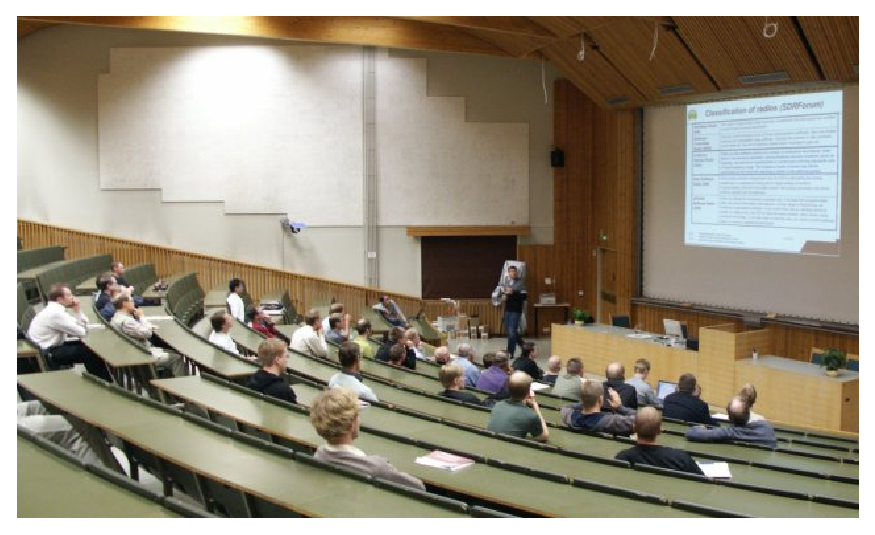
\includegraphics[height=8cm]{charts/kuva2}
\end{center}
\caption{Title \label{liitekuva}}
\end{figure}
%%

\begin{table}[htb]
\caption{table title \label{liitetaulukko}}
\begin{center}
\fbox{
\begin{tabular}{lp{0.5\linewidth}}
11 & 12  \\
21 & 22 \\
\end{tabular}}
\end{center}
\end{table}

\begin{eqnarray}
T_{ik} &=& -p g_{ik} + w u_i u_k + \tau_{ik},  \label{liitekaava3} \\
n_i    &=& n u_i + v_i.                        \label{liitekaava4}
\end{eqnarray}


\end{document}
